\documentclass[11pt,a4paper]{report}
% ==========================================================
%  Common preamble for the General Relativity documents
%  (IMAPP M1, Université Clermont Auvergne)
% ==========================================================
\usepackage[utf8]{inputenc}
\usepackage[T1]{fontenc}
\usepackage{lmodern}
\usepackage[english]{babel}
\usepackage[a4paper,margin=2.4cm,headheight=14pt]{geometry}
\usepackage{amsmath,amssymb,amsthm,mathtools}
\usepackage{bm}
\usepackage{enumitem}
\usepackage{booktabs}
\usepackage{array}
\usepackage{xcolor}
\usepackage{graphicx}
\usepackage{fancyhdr}
\usepackage{tikz}
\usetikzlibrary{arrows.meta,calc,decorations.pathmorphing,decorations.markings,patterns,shapes.geometric,positioning,3d,intersections}
\usepackage{pgfplots}
\pgfplotsset{compat=1.18}
\usepackage[most]{tcolorbox}
\usepackage[colorlinks=true,linkcolor=blue!50!black,citecolor=blue!50!black,urlcolor=blue!50!black]{hyperref}
\usepackage[capitalise,noabbrev]{cleveref}
\usepackage{caption}
\captionsetup{font=small,labelfont=bf}

\allowdisplaybreaks
\setlength{\parindent}{0pt}
\setlength{\parskip}{0.55em}
\numberwithin{equation}{section}

% ---------- colours ----------
\definecolor{defcol}{RGB}{0,90,160}
\definecolor{thmcol}{RGB}{160,40,40}
\definecolor{remcol}{RGB}{90,90,90}
\definecolor{excol}{RGB}{0,120,60}
\definecolor{warncol}{RGB}{200,110,0}

% ---------- boxes ----------
\tcbset{boxbase/.style={enhanced,breakable,sharp corners=south,boxrule=0.6pt,
    left=6pt,right=6pt,top=4pt,bottom=4pt,fonttitle=\bfseries,
    before skip=8pt,after skip=8pt}}
\newtcbtheorem[number within=section]{definition}{Definition}{boxbase,
    colback=defcol!4,colframe=defcol!70!black}{def}
\newtcbtheorem[use counter from=definition]{theorem}{Theorem}{boxbase,
    colback=thmcol!4,colframe=thmcol!70!black}{thm}
\newtcbtheorem[use counter from=definition]{proposition}{Proposition}{boxbase,
    colback=thmcol!4,colframe=thmcol!70!black}{prop}
\newtcbtheorem[use counter from=definition]{example}{Example}{boxbase,
    colback=excol!4,colframe=excol!70!black}{ex}
\newtcbtheorem[use counter from=definition]{exercise}{Exercise}{boxbase,
    colback=excol!4,colframe=excol!70!black}{exc}

\newtcolorbox{keyresult}[1][]{enhanced,breakable,colback=yellow!8,colframe=orange!70!black,
    boxrule=0.8pt,left=6pt,right=6pt,top=4pt,bottom=4pt,fonttitle=\bfseries,
    title={#1},before skip=8pt,after skip=8pt}
\newtcolorbox{remarkbox}[1][Remark]{enhanced,breakable,colback=remcol!5,colframe=remcol!70,
    boxrule=0.4pt,left=6pt,right=6pt,top=3pt,bottom=3pt,fonttitle=\bfseries\small,
    title={#1},before skip=6pt,after skip=6pt}
\newtcolorbox{warningbox}[1][Warning]{enhanced,breakable,colback=warncol!6,colframe=warncol!80!black,
    boxrule=0.6pt,left=6pt,right=6pt,top=3pt,bottom=3pt,fonttitle=\bfseries\small,
    title={#1},before skip=6pt,after skip=6pt}

\theoremstyle{remark}
\newtheorem*{proofsketch}{Proof sketch}

% ---------- macros ----------
\newcommand{\dd}{\mathrm{d}}
\newcommand{\pd}{\partial}
\newcommand{\R}{\mathbb{R}}
\newcommand{\M}{\mathcal{M}}
\newcommand{\Ga}[3]{\Gamma^{#1}{}_{#2#3}}
\newcommand{\Riem}[4]{R^{#1}{}_{#2#3#4}}
\newcommand{\tr}{\operatorname{tr}}
\newcommand{\sgn}{\operatorname{sgn}}
\newcommand{\GN}{G_{\mathrm N}}
\newcommand{\rs}{r_{\mathrm s}}
\newcommand{\eq}[1]{\begin{align}#1\end{align}}
\renewcommand{\Box}{\square}
\renewcommand{\vec}[1]{\bm{#1}}
\newcommand{\order}[1]{\mathcal{O}\!\left(#1\right)}
\newcommand{\half}{\tfrac12}


\pagestyle{fancy}
\fancyhf{}
\fancyhead[L]{\small\nouppercase{\leftmark}}
\fancyhead[R]{\small General Relativity --- Lecture Notes}
\fancyfoot[C]{\thepage}

\title{\Huge\bfseries General Relativity\\[0.4em]
\Large Complete Lecture Notes\\[1.2em]
\large IMAPP Master (M1) --- Université Clermont Auvergne}
\author{Based on the lectures of A.~Goudelis (LPCA),\\
the handwritten notes of Samuel and of a former student,\\
completed, expanded and typeset}
\date{Academic year 2026--2027}

\begin{document}
\maketitle
\thispagestyle{empty}

\chapter*{Preface}
\addcontentsline{toc}{chapter}{Preface}
These notes are a complete and expanded version of the General Relativity course of the IMAPP Master (M1).
They follow the structure of the lectures as recorded in the handwritten notes of Samuel, and they are completed,
for the last part of the course (black holes, cosmology and gravitational waves), with the notes of a former student.
Every derivation that was only sketched (or ``left as an exercise'') in the handwritten notes has been carried out
step by step, and many additional explanations, remarks and figures have been added.

\paragraph{Conventions.} Throughout these notes we use:
\begin{itemize}[nosep]
  \item the metric signature $(+,-,-,-)$, so that $\eta_{\mu\nu}=\mathrm{diag}(1,-1,-1,-1)$ and time-like vectors have positive norm;
  \item Greek indices $\mu,\nu,\dots\in\{0,1,2,3\}$ for space-time components and Latin indices $i,j,\dots\in\{1,2,3\}$ for spatial ones;
  \item the Einstein summation convention (an index appearing once up and once down is summed);
  \item $x^0=ct$; in some chapters we set $c=1$ (this is always stated explicitly);
  \item the Riemann tensor $\Riem{\rho}{\sigma}{\mu}{\nu}=\pd_\mu\Ga{\rho}{\nu}{\sigma}-\pd_\nu\Ga{\rho}{\mu}{\sigma}
        +\Ga{\rho}{\mu}{\lambda}\Ga{\lambda}{\nu}{\sigma}-\Ga{\rho}{\nu}{\lambda}\Ga{\lambda}{\mu}{\sigma}$,
        the Ricci tensor $R_{\mu\nu}=\Riem{\rho}{\mu}{\rho}{\nu}$, and the Ricci scalar $R=g^{\mu\nu}R_{\mu\nu}$;
  \item with these conventions the Einstein field equations read $R_{\mu\nu}-\tfrac12 g_{\mu\nu}R=\frac{8\pi \GN}{c^4}T_{\mu\nu}$.
\end{itemize}
When the former student's notes used the opposite signature $(-,+,+,+)$, all results have been translated to $(+,-,-,-)$.

\paragraph{How to read the boxes.}
Blue boxes contain definitions, red boxes theorems/propositions, green boxes examples and exercises,
yellow boxes the key results to remember, and grey boxes remarks.

\tableofcontents

\part{Introductory lectures}
% =====================================================================
\chapter{Introduction and the Equivalence Principle}
% =====================================================================

\section{Why General Relativity?}

Physics, as we know it today, describes Nature through \emph{four fundamental interactions}:
\begin{enumerate}[label=(\roman*)]
  \item \textbf{Electromagnetism}, described classically by Maxwell's equations and, at the quantum level, by Quantum Electrodynamics (QED);
  \item the \textbf{weak interaction}, responsible e.g.\ for $\beta$ decay;
  \item the \textbf{strong interaction}, described by Quantum Chromodynamics (QCD);
  \item \textbf{gravity}, described by Newtonian mechanics in the regime of weak fields and small velocities, and in full generality by \emph{General Relativity} (GR).
\end{enumerate}
The first two are unified, within the Standard Model (SM) of particle physics, into the \emph{electroweak theory},
based on the gauge group $SU(2)_L\times U(1)_Y$. Together with QCD (gauge group $SU(3)_c$) they form the SM,
which is a \emph{quantum} field theory. Gravity stands apart: General Relativity is a \emph{classical} (i.e.\ non-quantum) theory,
and no fully satisfactory quantum theory of gravity is known.

General Relativity is at the same time
\begin{itemize}[nosep]
  \item a \textbf{theory of gravity}, and
  \item a \textbf{theory of space-time} itself.
\end{itemize}
In Newtonian physics space and time are a fixed, absolute stage on which physics happens. In GR the stage becomes an actor:
the geometry of space-time is dynamical and is determined by its matter and energy content. This double role is beautifully summarised by J.\,A.~Wheeler:
\begin{quote}
\emph{``Space-time tells matter how to move; matter tells space-time how to curve.''}
\end{quote}
The first half of the sentence will be made precise by the \emph{geodesic equation} (\cref{ch:connection}), the second half by the \emph{Einstein field equations} (\cref{ch:efe}).

\section{Useful notions}

Before entering the subject we fix a few basic notions that will be used throughout the course.

\begin{definition}{Event}{event}
An \textbf{event} is a physical occurrence at a specific point of space and at a specific instant of time, i.e.\ associated with a specific space-time point.
An event has no spatial extension and no duration: it is a zero-dimensional object.
\end{definition}
\textit{Examples:} the emission of a photon by an atom; the presence of a point-like particle at a given place at a given time; two particles colliding.

\begin{definition}{Observer}{observer}
An \textbf{observer} is, essentially, a \emph{reference frame}: a way of assigning coordinates (three spatial coordinates and a time) to events.
\end{definition}
We can switch from one observer to another by means of \emph{coordinate transformations}. A central theme of the course is that physical statements must not depend on which observer (i.e.\ which coordinates) we use.

\begin{definition}{Local time}{localtime}
Each observer is equipped with an ideal standard clock and has a notion of time: he/she can assign a time to events and, therefore, a temporal ordering (``this event happened before that one'').
All observers measure time in the same way (with identical ideal clocks), even if, as we will see, they do not necessarily agree on the result.
\end{definition}

\begin{definition}{World-line}{worldline}
The \textbf{world-line} of a point-like object is the path that it follows in space-time. It is a one-dimensional object (a curve).
For extended objects one speaks of a \emph{world-sheet} (a string, 2D) or a \emph{world-volume} (higher-dimensional objects).
\end{definition}

% ---------------------------------------------------------------------
\section{The Equivalence Principle}
% ---------------------------------------------------------------------
The Equivalence Principle (EP) is the physical cornerstone on which Einstein built General Relativity. We first recall its Newtonian (Galilean) version and then formulate Einstein's version.

\subsection{The Newtonian (Galilean) version}

Consider a body of mass $m$, located at a point $P$ near the surface of the Earth. In Newtonian physics two \emph{a priori} completely different notions of mass enter its description:
\begin{itemize}
  \item From \textbf{Newtonian gravity}, the gravitational force acting on the body is
  \begin{equation}
    \vec F = -m_g\,\nabla\phi ,
  \end{equation}
  where $\phi$ is the gravitational potential and $m_g$ is the \textbf{gravitational mass}.
  It plays for gravity the role that the electric charge plays for electromagnetism ($\vec F=q\vec E=-q\nabla V$): it is a kind of ``gravitational charge'', measuring how strongly the body couples to the gravitational field.
  \item From \textbf{Newtonian mechanics} (Newton's second law),
  \begin{equation}
    \vec F = m_i\,\vec a ,
  \end{equation}
  where $m_i$ is the \textbf{inertial mass}. It tells us how much the body \emph{resists} being accelerated by \emph{any} force.
\end{itemize}

\begin{figure}[ht]
\centering
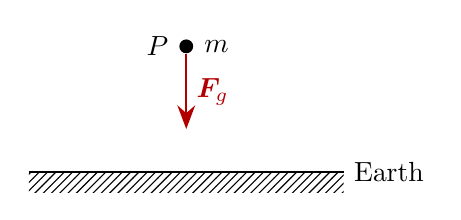
\begin{tikzpicture}[scale=1]
  \fill[pattern=north east lines] (-2,-0.25) rectangle (2,0);
  \draw[thick] (-2,0) -- (2,0) node[right] {Earth};
  \fill (0,1.6) circle (2.5pt) node[left=3pt] {$P$} node[right=3pt] {$m$};
  \draw[-{Stealth[length=3mm]},thick,red!70!black] (0,1.5) -- (0,0.55) node[midway,right] {$\vec F_g$};
\end{tikzpicture}
\caption{A body of mass $m$ at a point $P$ above the surface of the Earth, subject to the gravitational force $\vec F_g$.}
\label{fig:newton-ep}
\end{figure}

There is no reason, within Newtonian theory, for these two quantities to be equal: they are \emph{fundamentally different} concepts. Yet, experimentally, one observes (to an extremely high precision: $|m_i-m_g|/m_i\lesssim 10^{-15}$ in modern torsion-balance and space experiments) that
\begin{equation}
  m_i = m_g
\end{equation}
(more precisely, they are proportional to each other with a universal constant, which can be absorbed into the definition of Newton's constant $\GN$ and set to one).

\begin{keyresult}[Galilean Equivalence Principle]
The inertial and the gravitational masses of any body are equal, $m_i=m_g$. Consequently, equating the two expressions of the force,
\begin{equation}
  m_i\,\vec a = -m_g\,\nabla\phi \quad\Longrightarrow\quad \vec a = -\nabla\phi ,
\end{equation}
\emph{independently of the mass and of the composition of the body}. This is the \textbf{universality of free fall}: all bodies fall in the same way in a gravitational field (Galileo's experiments, the hammer and the feather on the Moon, \dots). In other words, \emph{the motion in a gravitational field does not depend on the mass}.
\end{keyresult}

This is a very peculiar property of gravity: for the electric force, $\vec a=(q/m)\vec E$ depends on the charge-to-mass ratio of the body, so different bodies fall differently in an electric field.

\subsection{Einstein's version of the Equivalence Principle}

Einstein's insight was to take the universality of free fall seriously and to turn it into a principle about \emph{reference frames}. Consider an elevator (a closed box) containing a particle of mass $m$ at a point $P$. We introduce two frames (see \cref{fig:elevator}):
\begin{itemize}[nosep]
  \item $R$, a ``static'' frame with coordinates $(x,z)$;
  \item $R'$, a frame \emph{comoving} with the elevator, with coordinates $(x',z')$.
\end{itemize}

\begin{figure}[ht]
\centering
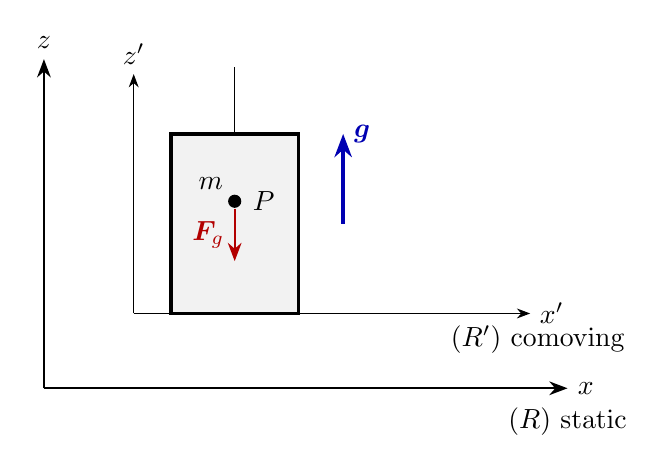
\begin{tikzpicture}[scale=0.95,>=Stealth]
  % static frame R
  \draw[->,thick] (0,0) -- (7,0) node[right] {$x$};
  \draw[->,thick] (0,0) -- (0,4.4) node[above] {$z$};
  \node at (7.0,-0.45) {$(R)$ static};
  % comoving frame R'
  \draw[->] (1.2,1.0) -- (6.5,1.0) node[right] {$x'$};
  \draw[->] (1.2,1.0) -- (1.2,4.2) node[above] {$z'$};
  \node at (6.6,0.65) {$(R')$ comoving};
  % elevator
  \draw[very thick,fill=gray!10] (1.7,1.0) rectangle (3.4,3.4);
  \draw (2.55,3.4) -- (2.55,4.3); % rope
  \fill (2.55,2.5) circle (2.5pt) node[right=3pt] {$P$} node[above left=1pt] {$m$};
  \draw[->,thick,red!70!black] (2.55,2.4) -- (2.55,1.7) node[midway,left] {$\vec F_g$};
  \draw[->,very thick,blue!70!black] (4.0,2.2) -- (4.0,3.4) node[right] {$\vec g$};
\end{tikzpicture}
\caption{Einstein's elevator. $R$ is a static frame, $R'$ is the frame comoving with the elevator. Depending on the case, the elevator is at rest in empty space, uniformly accelerated (acceleration $\vec g$ upwards), or at rest in a uniform gravitational field (force $\vec F_g$ downwards on the particle).}
\label{fig:elevator}
\end{figure}

We consider the following situations.
\begin{description}
  \item[Case 0.] The elevator is in outer space, far from any mass, and no force acts on it. Then the particle simply \emph{floats} inside the elevator.
  \item[Case 1.] Still in outer space, but now the elevator is accelerated upwards with a constant acceleration $\vec g$ (e.g.\ by a rocket). Then the particle (which feels no force) is approached by the floor of the elevator: for an observer in the elevator, the particle ``falls'' towards the floor with acceleration $-\vec g$.
  \item[Case 2.] The elevator is at rest, but inside a constant gravitational field $\vec g$ pointing downwards (e.g.\ at rest on the surface of the Earth). Again, the particle approaches the floor with acceleration $-\vec g$.
\end{description}
Both $R$ and $R'$ agree on these statements. \textbf{But} the observer in $R'$ \emph{cannot distinguish case 1 from case 2} by any experiment performed inside the elevator. Hence:
\begin{center}
\fbox{\textsc{Gravity} $=$ \textsc{Acceleration}}
\end{center}
(locally, see below).

\paragraph{Quantitative version of case 1.} Let us neglect special-relativistic effects (so that $t'=t$). In $R$ the elevator floor moves as $z_{\rm floor}(t)=\tfrac12 g t^2$, so that $\ddot z_{\rm floor}=g$. The coordinates of the two frames are related by
\begin{equation}
  z' = z-\tfrac12 g t^2,\qquad x'=x,\qquad t'=t .
\end{equation}
Differentiating twice with respect to time, $\ddot z'=\ddot z-g$. In $R$, Newton's law reads $F=m\ddot z$. In $R'$,
\begin{equation}
  F' \equiv m\ddot z' = m\ddot z - mg \quad\Longrightarrow\quad F' = F - mg .
\end{equation}
The acceleration of $R'$ with respect to $R$ manifests itself in $R'$ as an additional force $-mg$, which is \emph{exactly} what a uniform gravitational field would produce. Note that this ``inertial force'' is proportional to the inertial mass, whereas gravity is proportional to the gravitational mass: their indistinguishability is precisely $m_i=m_g$.

\begin{description}
  \item[Case 3.] The elevator is in the gravitational field of the Earth and we cut the rope, so that it falls freely. Then the particle \emph{floats} with respect to $R'$, exactly as in case 0: the observer in $R'$ cannot tell whether he/she is at rest in outer space or freely falling in a gravitational field. Freely falling frames are locally equivalent to inertial frames: gravity has been ``switched off'' by going to a freely-falling frame.
\end{description}

\begin{keyresult}[Einstein's Equivalence Principle]
No physical experiment can distinguish \emph{locally} between a uniform gravitational field acting on a local inertial observer and a uniform acceleration with respect to that local inertial observer.

Here the \emph{local inertial observer} is the one for whom Special Relativity holds (a freely-falling observer).
\end{keyresult}

\subsection{Why ``locally''?}

Real gravitational fields are not uniform: the gravitational field of the Earth points towards its centre and its strength decreases with the distance. Consider a large freely-falling elevator (or two elevators at different positions, see \cref{fig:locally}). Two particles initially at rest at the two ends of a horizontal elevator both fall towards the centre of the Earth, along \emph{non-parallel} directions: seen from inside the elevator, they slowly approach each other. Similarly, two particles at different heights in a vertical elevator feel slightly different accelerations and drift apart. These \emph{tidal effects} cannot be removed by changing reference frame: they are the genuine signature of a gravitational field, and they will turn out to be the manifestation of space-time \emph{curvature} (\cref{sec:geodesic-deviation}).

\begin{figure}[ht]
\centering
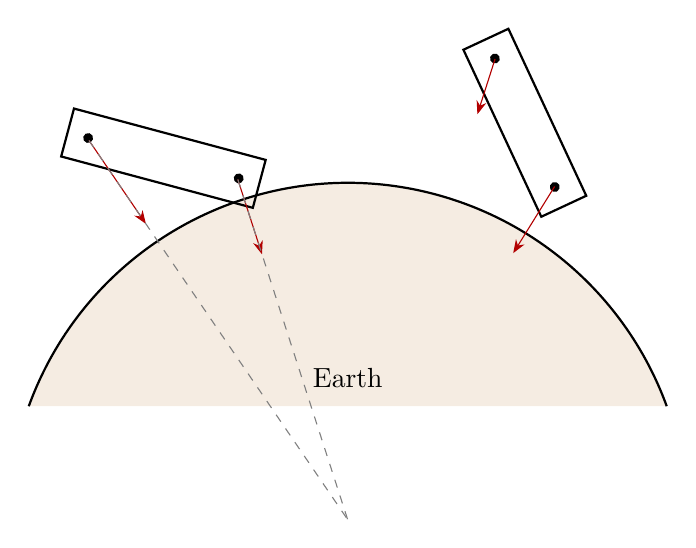
\begin{tikzpicture}[scale=0.9,>=Stealth]
  \draw[thick,fill=brown!15] (-4.5,0) arc (160:20:4.79) ;
  \node at (0,0.4) {Earth};
  \coordinate (C) at (0,-1.6);
  % horizontal elevator (left)
  \begin{scope}[shift={(-2.6,3.5)},rotate=-15]
    \draw[thick] (-1.4,-0.35) rectangle (1.4,0.35);
    \fill (-1.1,0) circle (2pt); \fill (1.1,0) circle (2pt);
  \end{scope}
  \draw[->,red!70!black] (-3.65,3.75) -- ($(-3.65,3.75)!0.22!(C)$);
  \draw[->,red!70!black] (-1.55,3.2) -- ($(-1.55,3.2)!0.22!(C)$);
  % vertical elevator (right)
  \begin{scope}[shift={(2.5,4.0)},rotate=25]
    \draw[thick] (-0.35,-1.3) rectangle (0.35,1.3);
    \fill (0,1.0) circle (2pt); \fill (0,-1.0) circle (2pt);
  \end{scope}
  \draw[->,red!70!black] (2.08,4.9) -- ($(2.08,4.9)!0.12!(C)$);
  \draw[->,red!70!black] (2.92,3.1) -- ($(2.92,3.1)!0.2!(C)$);
  \draw[dashed,gray] (-3.65,3.75) -- (C);
  \draw[dashed,gray] (-1.55,3.2) -- (C);
\end{tikzpicture}
\caption{Why the Equivalence Principle only holds locally. In a freely-falling elevator, test particles fall towards the centre of the Earth along converging directions (left) and with height-dependent accelerations (right): these tidal effects cannot be removed by a change of frame.}
\label{fig:locally}
\end{figure}

\subsection{First consequence: light bends in a gravitational field}

Consider again the elevator accelerated upwards with acceleration $\vec g$ (case 1), and a laser fixed on the left wall that emits a light pulse horizontally (\cref{fig:lightbend}). In the inertial frame $R$ the light travels in a straight line. During the time the light needs to cross the elevator, however, the elevator has moved upwards: in $R'$ the light enters at the point $P_1$ and hits the opposite wall at a point $P_2$ which is \emph{lower} than $P_1$. Hence, in the accelerated frame, light follows a curved (parabolic) trajectory.

By the Equivalence Principle the same must happen in an elevator at rest in a gravitational field: \textbf{light feels gravity, and light bends}. This is a striking prediction, since photons are massless; it will be computed quantitatively in \cref{sec:light-bending}.

\begin{figure}[ht]
\centering
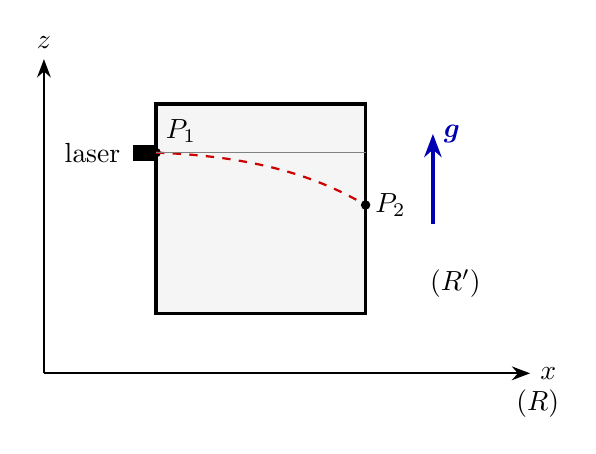
\begin{tikzpicture}[scale=0.95,>=Stealth]
  \draw[->,thick] (0,0) -- (6.5,0) node[right] {$x$};
  \draw[->,thick] (0,0) -- (0,4.2) node[above] {$z$};
  \node at (6.6,-0.4) {$(R)$};
  \draw[very thick,fill=gray!8] (1.5,0.8) rectangle (4.3,3.6);
  \draw[fill=black] (1.2,2.85) rectangle (1.5,3.05);
  \node[left] at (1.15,2.95) {laser};
  \fill (1.5,2.95) circle (1.8pt) node[above right] {$P_1$};
  \draw[thick,red!80!black,dashed] (1.5,2.95) .. controls (2.9,2.9) and (3.7,2.6) .. (4.3,2.25);
  \fill (4.3,2.25) circle (1.8pt) node[right] {$P_2$};
  \draw[gray,thin] (1.5,2.95) -- (4.3,2.95);
  \draw[->,very thick,blue!70!black] (5.2,2.0) -- (5.2,3.2) node[right] {$\vec g$};
  \node at (5.5,1.2) {$(R')$};
\end{tikzpicture}
\caption{A light ray emitted horizontally in an elevator accelerated upwards. In the comoving frame $R'$ the ray hits the opposite wall at $P_2$, lower than the emission height $P_1$: light bends. By the EP the same happens in a gravitational field.}
\label{fig:lightbend}
\end{figure}

\subsection{Second consequence: the gravitational redshift}\label{sec:redshift-ep}

Consider a tower of height $d$ in a uniform gravitational field $g$. A photon of frequency $f_P$ is emitted by an emitter $P$ at the bottom and detected by a detector $Q$ at the top. Which frequency $f_Q$ does $Q$ measure?

By the EP, we can replace the gravitational field by an elevator accelerated upwards with acceleration $g$, in which $P$ and $Q$ are at rest and separated by the distance $d$ (\cref{fig:redshift}). We work to first order in $gd/c^2\ll 1$.
\begin{itemize}
  \item The time of flight of the photon is $\Delta t= d/c$.
  \item During this time, the velocity of the elevator (hence of the detector $Q$ with respect to the inertial frame in which the emitter was at rest at the moment of emission) increases by
  \begin{equation}
    \Delta v = g\,\Delta t = \frac{g d}{c}.
  \end{equation}
  \item The detector is therefore moving \emph{away} from the point of emission with velocity $\Delta v$ when it receives the photon, and it observes a Doppler-shifted frequency (non-relativistic Doppler effect, since $\Delta v\ll c$):
  \begin{equation}
    \frac{f_Q}{f_P} = 1-\frac{\Delta v}{c} = 1-\frac{g d}{c^2}.
  \end{equation}
\end{itemize}

\begin{figure}[ht]
\centering
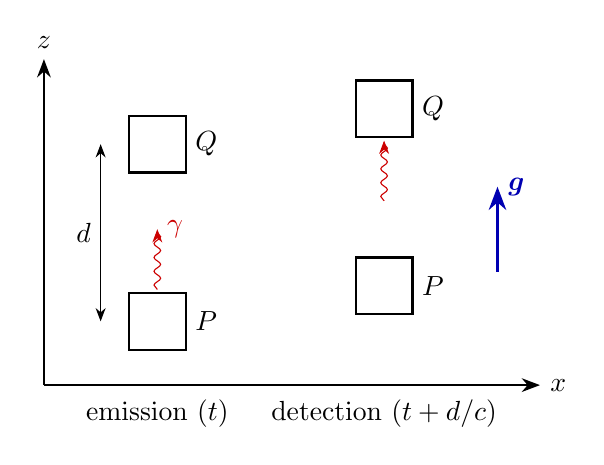
\begin{tikzpicture}[scale=0.9,>=Stealth]
  \draw[->,thick] (0,0) -- (7,0) node[right] {$x$};
  \draw[->,thick] (0,0) -- (0,4.6) node[above] {$z$};
  % at emission
  \draw[thick] (1.2,0.5) rectangle (2.0,1.3); \node[right] at (2.0,0.9) {$P$};
  \draw[thick] (1.2,3.0) rectangle (2.0,3.8); \node[right] at (2.0,3.4) {$Q$};
  \draw[<->] (0.8,0.9) -- (0.8,3.4) node[midway,left] {$d$};
  \draw[decorate,decoration={snake,amplitude=1.2pt,segment length=5pt},->,red!80!black] (1.6,1.35) -- (1.6,2.2) node[right] {$\gamma$};
  \node at (1.6,-0.4) {emission ($t$)};
  % at detection
  \draw[thick] (4.4,1.0) rectangle (5.2,1.8); \node[right] at (5.2,1.4) {$P$};
  \draw[thick] (4.4,3.5) rectangle (5.2,4.3); \node[right] at (5.2,3.9) {$Q$};
  \draw[decorate,decoration={snake,amplitude=1.2pt,segment length=5pt},->,red!80!black] (4.8,2.6) -- (4.8,3.45);
  \node at (4.8,-0.4) {detection ($t+d/c$)};
  \draw[->,very thick,blue!70!black] (6.4,1.6) -- (6.4,2.8) node[right] {$\vec g$};
\end{tikzpicture}
\caption{Gravitational redshift via the Equivalence Principle: emitter $P$ and detector $Q$, separated by $d$, are accelerated upwards with acceleration $g$. During the photon's time of flight $d/c$ the detector gains a velocity $\Delta v=gd/c$.}
\label{fig:redshift}
\end{figure}

\begin{keyresult}[Gravitational redshift]
By the Equivalence Principle (acceleration $\leftrightarrow$ gravity), in the presence of a uniform gravitational field and in a fixed reference frame, a photon climbing a height $d$ is redshifted:
\begin{equation}
  \frac{f_Q}{f_P} = 1-\frac{g d}{c^2} = 1-\frac{\Delta\phi}{c^2},\qquad \Delta\phi=\phi_Q-\phi_P = g d .
\end{equation}
\end{keyresult}

\paragraph{Interpretation in terms of clocks.} The number of wave crests is conserved between emission and reception (in a static situation nothing accumulates between $P$ and $Q$). The fact that $Q$ counts fewer crests per unit of its own time than $P$ emits per unit of its own time means that the two clocks do not tick at the same rate: equivalently, \textbf{clocks at lower gravitational potential tick slower}. A clock at the bottom ($P$), seen from the top ($Q$), runs slow by the factor $1-gd/c^2$ (and, conversely, the clock at $Q$ appears to run fast when seen from $P$). Time itself flows differently at different heights: gravity affects the geometry of \emph{space-time}, not just the motion of bodies. This effect has been measured in the Pound--Rebka experiment (1959) and is routinely taken into account by the GPS system.

% =====================================================================
\chapter{Recap of Special Relativity: vectors and tensors}\label{ch:sr}
% =====================================================================

In this chapter we recall Special Relativity (SR), emphasising the language of vectors and tensors.
Everything here will later be generalised to curved space-time; it is therefore worth understanding it well in the simpler setting of flat space-time.

\section{Space-time, events and the line element}

In SR space and time are treated jointly as a single entity, \textbf{space-time}.

\paragraph{1. Events.} Events in space-time are labelled by three Cartesian coordinates $\{x^k\}$, $k=1,2,3$, describing Euclidean space, plus a time coordinate $x^0\equiv ct$. Collectively,
\begin{equation}
  (x^\mu) = (ct,x^1,x^2,x^3) = (ct,\vec x).
\end{equation}
The space-time of SR is called \textbf{Minkowski space-time}.

\paragraph{2. Distances.} Distances in Minkowski space-time are measured by means of the \textbf{line element}
\begin{equation}
  \dd s^2 \equiv (\dd x^0)^2-\sum_{i=1}^{3}(\dd x^i)^2 = c^2\dd t^2-\dd\vec x^{\,2} .
  \label{eq:line-element-mink}
\end{equation}
For a massive particle, $\dd s^2=c^2\dd\tau^2$ where $\tau$ is its proper time (see below).
\begin{remarkbox}[Alternative convention]
Many textbooks (and part of the former student's notes) use the opposite sign, $\dd s^2=-(\dd x^0)^2+\sum_i(\dd x^i)^2$ (signature $(-,+,+,+)$). Physics does not depend on this choice, but signs in intermediate formulae do. In these notes we always use $(+,-,-,-)$.
\end{remarkbox}

\paragraph{3. The metric tensor.} We introduce the (Minkowski) \textbf{metric tensor}
\begin{equation}
  \eta_{\mu\nu}=\begin{pmatrix} 1&0&0&0\\0&-1&0&0\\0&0&-1&0\\0&0&0&-1\end{pmatrix}
  \qquad\Longrightarrow\qquad
  \dd s^2=\sum_{\mu,\nu=0}^{3}\eta_{\mu\nu}\,\dd x^\mu\dd x^\nu .
\end{equation}
\textit{Index conventions:} Latin indices $i,j,k,\dots$ take the values $1,2,3$; Greek indices $\mu,\nu,\dots$ take the values $0,1,2,3$.

\paragraph{4. Einstein summation convention.} Any index that appears \emph{both as an upper and as a lower index} in a monomial is summed over:
\begin{equation}
  \dd s^2=\eta_{\mu\nu}\dd x^\mu\dd x^\nu\equiv\sum_{\mu,\nu}\eta_{\mu\nu}\dd x^\mu\dd x^\nu .
\end{equation}
A summed index is called a \emph{dummy} index: it can be renamed at will ($A_\mu B^\mu=A_\alpha B^\alpha$). An index that is not summed is a \emph{free} index: it must appear in the same position on both sides of an equation.

\section{Lorentz and Poincaré transformations}

\paragraph{5. Lorentz transformations} are the \emph{linear} transformations
\begin{equation}
  x^\mu\;\longrightarrow\; x'^\mu = L^\mu{}_\nu\,x^\nu
\end{equation}
that leave the line element invariant:
\begin{equation}
  \dd s'^2=\eta_{\mu\nu}\dd x'^\mu\dd x'^\nu \overset{!}{=}\eta_{\mu\nu}\dd x^\mu\dd x^\nu=\dd s^2 .
\end{equation}
Note that the metric is the \emph{same} matrix $\eta_{\mu\nu}$ in both frames: this is what characterises inertial frames in SR.

\begin{proposition}{Defining property of Lorentz transformations}{lorentz-cond}
A linear transformation $L$ is a Lorentz transformation if and only if
\begin{equation}
  \eta_{\mu\nu}\,L^\mu{}_\alpha\,L^\nu{}_\beta=\eta_{\alpha\beta}
  \qquad\Longleftrightarrow\qquad L^{T}\eta L=\eta \ \ (\text{matrix form}).
  \label{eq:lorentz-cond}
\end{equation}
\end{proposition}
\begin{proof}
Since $\dd x'^\mu=L^\mu{}_\alpha\dd x^\alpha$ (the transformation is linear with constant coefficients),
\[
  \dd s'^2=\eta_{\mu\nu}\dd x'^\mu\dd x'^\nu=\eta_{\mu\nu}L^\mu{}_\alpha\dd x^\alpha L^\nu{}_\beta\dd x^\beta
  =\big(\eta_{\mu\nu}L^\mu{}_\alpha L^\nu{}_\beta\big)\dd x^\alpha\dd x^\beta .
\]
On the other hand $\dd s^2=\eta_{\alpha\beta}\dd x^\alpha\dd x^\beta$. Requiring $\dd s'^2=\dd s^2$ for \emph{all} displacements $\dd x^\alpha$, and since both coefficient matrices are symmetric in $(\alpha,\beta)$, the coefficients must coincide (the argument is the same as the one detailed in \cref{prop:metric-transf}), which gives \eqref{eq:lorentz-cond}.
\end{proof}

\begin{example}{Boost along $x$}{boost}
With $\beta=v/c$ and $\gamma=(1-\beta^2)^{-1/2}$,
\[
L^\mu{}_\nu=\begin{pmatrix}\gamma&-\gamma\beta&0&0\\-\gamma\beta&\gamma&0&0\\0&0&1&0\\0&0&0&1\end{pmatrix},
\qquad ct'=\gamma(ct-\beta x),\quad x'=\gamma(x-\beta ct).
\]
One checks $L^T\eta L=\eta$: e.g.\ the $(0,0)$ component gives $\gamma^2-\gamma^2\beta^2=1$, the $(0,1)$ component $-\gamma^2\beta+\gamma^2\beta=0$, and the $(1,1)$ component $\gamma^2\beta^2-\gamma^2=-1$.
\end{example}

\begin{remarkbox}[Remarks]
\begin{enumerate}[nosep]
  \item Lorentz transformations combined with space-time translations form the \textbf{Poincaré transformations}:
  $x^\mu\to x'^\mu=L^\mu{}_\nu x^\nu+\xi^\mu$, with constant $\xi^\mu$. They also leave $\dd s^2$ invariant, since $\dd\xi^\mu=0$.
  \item Any two inertial frames are related through a Poincaré transformation.
  \item Lorentz (resp.\ Poincaré) transformations form a \emph{group}: the product of two of them is again one of them ($(L_1L_2)^T\eta L_1L_2=L_2^TL_1^T\eta L_1L_2=L_2^T\eta L_2=\eta$), the identity belongs to the set, and every $L$ has an inverse (taking the determinant of \eqref{eq:lorentz-cond}, $(\det L)^2=1$).
\end{enumerate}
\end{remarkbox}

\section{Causal structure: the light cone}

\paragraph{6. The interval between two events.} For two events $P$ and $Q$ we define
\begin{equation}
  \Delta x^2\equiv\eta_{\mu\nu}(x_P^\mu-x_Q^\mu)(x_P^\nu-x_Q^\nu),
\end{equation}
which is Lorentz invariant. We say that $P$ and $Q$ are
\begin{itemize}[nosep]
  \item \textbf{time-like} separated if $\Delta x^2>0$;
  \item \textbf{light-like} (or null) separated if $\Delta x^2=0$;
  \item \textbf{space-like} separated if $\Delta x^2<0$.
\end{itemize}
The set of events light-like separated from $P$ forms the \textbf{light cone} of $P$ (\cref{fig:lightcone}). Events inside the cone can be causally connected with $P$ (a signal travelling at speed $<c$ can link them, and all observers agree on their time ordering). Events outside the cone cannot: their time ordering depends on the observer.

\begin{figure}[ht]
\centering
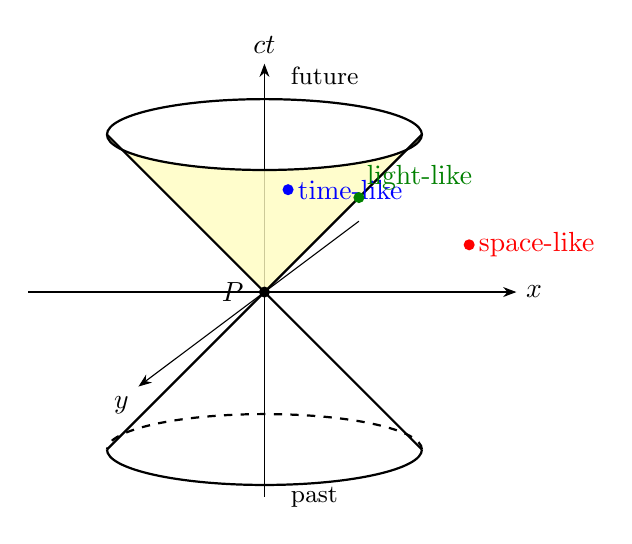
\begin{tikzpicture}[scale=1.0,>=Stealth]
  \draw[->] (-3,0) -- (3.2,0) node[right] {$x$};
  \draw[->] (0,-2.6) -- (0,2.9) node[above] {$ct$};
  \draw[->] (1.2,0.9) -- (-1.6,-1.2) node[below left] {$y$};
  % cone
  \fill[yellow!25,opacity=0.8] (0,0) -- (-2,2) arc (180:360:2 and 0.45) -- cycle;
  \draw[thick] (-2,2) -- (2,-2); \draw[thick] (2,2) -- (-2,-2);
  \draw[thick] (0,2) ellipse (2 and 0.45);
  \draw[thick,dashed] (2,-2) arc (0:180:2 and 0.45);
  \draw[thick] (-2,-2) arc (180:360:2 and 0.45);
  \fill (0,0) circle (2pt) node[left=4pt] {$P$};
  \fill[blue] (0.3,1.3) circle (2pt) node[right,blue] {time-like};
  \fill[red] (2.6,0.6) circle (2pt) node[right,red] {space-like};
  \fill[green!50!black] (1.2,1.2) circle (2pt) node[above right=-1pt,green!50!black] {light-like};
  \node at (0,2.75) [right=6pt] {\small future};
  \node at (0,-2.6) [right=6pt] {\small past};
\end{tikzpicture}
\hspace{1cm}
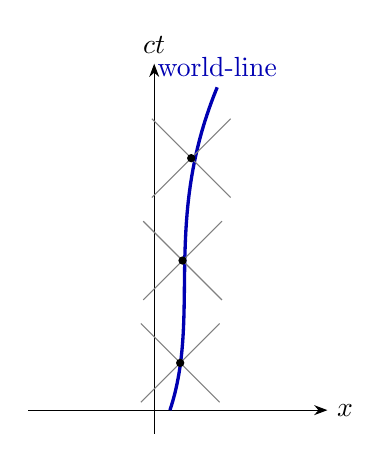
\begin{tikzpicture}[scale=1.0,>=Stealth]
  \draw[->] (-1.6,0) -- (2.2,0) node[right] {$x$};
  \draw[->] (0,-0.3) -- (0,4.4) node[above] {$ct$};
  \draw[very thick,blue!70!black] (0.2,0) .. controls (0.6,1.2) and (0.1,2.4) .. (0.8,4.1) node[above] {world-line};
  \foreach \t/\x in {0.6/0.33,1.9/0.36,3.2/0.47}{
     \draw[gray] (\x-0.5,\t-0.5) -- (\x+0.5,\t+0.5);
     \draw[gray] (\x+0.5,\t-0.5) -- (\x-0.5,\t+0.5);
     \fill (\x,\t) circle (1.5pt);}
\end{tikzpicture}
\caption{Left: the light cone of an event $P$ separates the events that are time-like (inside), light-like (on the cone) and space-like (outside) separated from $P$. Right: the world-line of a massive particle is everywhere time-like: at each of its points it lies inside the local light cone.}
\label{fig:lightcone}
\end{figure}

\section{Curves and tangent vectors}

\paragraph{7. Curves.} A \textbf{parametrised curve} $\mathcal C$ is given by a map $\lambda\mapsto x^\mu(\lambda)$, $\lambda\in I\subseteq\R$. The components of its \textbf{tangent vector} at $\lambda_0$ are
\begin{equation}
  V^\mu(\lambda_0)=\left.\frac{\dd x^\mu}{\dd\lambda}\right|_{\lambda=\lambda_0}.
\end{equation}

\begin{remarkbox}[Reparametrisations]
A curve $\mathcal C(I)$ can also be parametrised by a different parameter $\sigma\in J\subseteq\R$, via a bijective (smooth, with smooth inverse) map $\psi:I\to J$, $\sigma=\psi(\lambda)$. The new parametrisation $\mathcal C'=\mathcal C\circ\psi^{-1}$ satisfies $\mathcal C'(J)=\mathcal C(I)$: it describes \emph{the same curve} (the same set of points), traversed with a different ``speed''. The tangent vector is rescaled, $\dd x^\mu/\dd\sigma=(\dd\lambda/\dd\sigma)\,\dd x^\mu/\dd\lambda$.
\end{remarkbox}

A particularly convenient choice for a time-like curve is the \textbf{proper time} $\tau$,
\begin{equation}
  c\,\dd\tau=\sqrt{\eta_{\mu\nu}\dd x^\mu\dd x^\nu}.
\end{equation}
Why is it a good choice? (i) It is the time measured by an observer in his/her own (instantaneous rest) frame, by a clock carried along the curve; (ii) it is \textbf{Lorentz invariant}, since $\dd s^2$ is. As a consequence, the tangent vector with respect to $\tau$ transforms \emph{linearly} under Lorentz transformations:
\begin{equation}
  \frac{\dd}{\dd\tau'}x'^\mu(\tau')=\frac{\dd}{\dd\tau}x'^\mu(\tau)
  =\frac{\pd x'^\mu}{\pd x^\nu}\frac{\dd x^\nu}{\dd\tau}=L^\mu{}_\nu\frac{\dd x^\nu}{\dd\tau},
\end{equation}
where in the first step we used $\tau'=\tau$ and in the second the chain rule.

\section{Lorentz vectors, covectors and tensors}

\paragraph{8. Lorentz vectors} are objects whose components transform, under Lorentz transformations, as
\begin{equation}
  V'^\mu=L^\mu{}_\nu V^\nu .
\end{equation}
\begin{remarkbox}[Remarks]
\begin{enumerate}[nosep]
\item $L^\mu{}_\nu$ can (and should) be thought of as the \emph{Jacobian} of the transformation $x\to x'$: $L^\mu{}_\nu=\pd x'^\mu/\pd x^\nu$. This is what will generalise to arbitrary coordinate transformations.
\item From now on, the components of vectors carry \emph{upper} indices.
\end{enumerate}
\end{remarkbox}

\paragraph{9. Scalar product.} The metric defines a scalar product of two vectors $V,W$ and a (squared) norm:
\begin{equation}
  V\cdot W\equiv\eta_{\mu\nu}V^\mu W^\nu,\qquad V^2\equiv\eta_{\mu\nu}V^\mu V^\nu .
\end{equation}
Both are \textbf{Lorentz invariant}: $\eta_{\mu\nu}V'^\mu W'^\nu=\eta_{\mu\nu}L^\mu{}_\alpha L^\nu{}_\beta V^\alpha W^\beta=\eta_{\alpha\beta}V^\alpha W^\beta$ by \eqref{eq:lorentz-cond}. Vectors are called time-like, light-like or space-like according to the sign of their norm, as for intervals.

\paragraph{10. Covectors} are objects whose components transform with the \emph{dual} (transposed inverse) representation of the Lorentz group,
\begin{equation}
  \Lambda\equiv(L^T)^{-1}.
\end{equation}
Since $L^T\eta L=\eta$, we have $L^T\eta=\eta L^{-1}$, i.e.\ $L^T=\eta L^{-1}\eta^{-1}$ and therefore
\begin{equation}
  \Lambda=(L^T)^{-1}=\eta L\eta^{-1}.
\end{equation}
In index notation we denote the inverse metric by upper indices, $\eta^{\mu\nu}\equiv(\eta^{-1})^{\mu\nu}$ (numerically $\eta^{\mu\nu}=\eta_{\mu\nu}$), so that
\begin{equation}
  V'_\mu=\Lambda_\mu{}^\nu V_\nu,\qquad \Lambda_\mu{}^\nu=\eta_{\mu\alpha}L^\alpha{}_\beta\,\eta^{\beta\nu}.
  \label{eq:covector-lorentz}
\end{equation}
Covectors carry \emph{lower} indices. Given a vector $V^\mu$ and the metric we can always form the covector $V_\mu\equiv\eta_{\mu\nu}V^\nu$ (note that numerically $V_\mu\neq V^\mu$ in general: $V_\mu=(V^0,-\vec V)$).

\begin{example}{Lowering an index gives a covector}{lower}
Show that the object with components $U_\alpha=\eta_{\alpha\beta}V^\beta$, where $V^\beta$ are the components of a vector, is a covector.

\textit{Proof.} We have to see how its components transform:
\[
  U'_\alpha=\eta_{\alpha\beta}V'^\beta=\eta_{\alpha\beta}L^\beta{}_\nu V^\nu. \tag{1}
\]
Inverting the definition, $V^\nu=\eta^{\nu\delta}U_\delta$ (2). Inserting (2) in (1) and using \eqref{eq:covector-lorentz} (3):
\[
U'_\alpha=\eta_{\alpha\beta}L^\beta{}_\nu\eta^{\nu\delta}U_\delta=\Lambda_\alpha{}^\delta U_\delta . \qquad\blacksquare
\]
\end{example}

\begin{example}{The gradient is a covector}{gradient}
Show that $w_\mu=\pd\phi/\pd x^\mu$, where $\phi(x)$ is a scalar function, is a covector.

\textit{Proof.} By the chain rule,
\[
  w'_\mu=\frac{\pd\phi}{\pd x'^\mu}=\frac{\pd x^\nu}{\pd x'^\mu}\frac{\pd\phi}{\pd x^\nu}=\frac{\pd x^\nu}{\pd x'^\mu}w_\nu .
\]
Since $x'=Lx$, $x=L^{-1}x'$ and $\pd x^\nu/\pd x'^\mu=(L^{-1})^\nu{}_\mu$. From $L^T\eta L=\eta$ we get $L^{-1}=\eta^{-1}L^T\eta$, i.e.\ $(L^{-1})^\nu{}_\mu=\eta^{\nu\alpha}L^\beta{}_\alpha\eta_{\beta\mu}=\Lambda_\mu{}^\nu$. Hence $w'_\mu=\Lambda_\mu{}^\nu w_\nu$. $\blacksquare$
\end{example}

\begin{remarkbox}[Components versus geometric objects]
A vector can be written as $V=V^\mu e_{(\mu)}$, where $e_{(\mu)}$ are basis vectors. The \emph{components} $V^\mu$ are coordinate (basis) dependent, but the object $V$ itself is \textbf{not}: vectors exist regardless of the basis. When we change frame, components and basis vectors change in compensating ways.
\end{remarkbox}

\paragraph{11. Lorentz $(p,q)$ tensors} are objects with components $T^{\alpha_1\dots\alpha_p}{}_{\beta_1\dots\beta_q}$ transforming as
\begin{equation}
  T'^{\alpha_1\dots\alpha_p}{}_{\beta_1\dots\beta_q}=
  L^{\alpha_1}{}_{\mu_1}\cdots L^{\alpha_p}{}_{\mu_p}\,
  \Lambda_{\beta_1}{}^{\nu_1}\cdots\Lambda_{\beta_q}{}^{\nu_q}\,
  T^{\mu_1\dots\mu_p}{}_{\nu_1\dots\nu_q},
\end{equation}
i.e.\ as the product of $p$ vectors and $q$ covectors. Examples:
\begin{itemize}[nosep]
  \item $\eta_{\mu\nu}$ is a $(0,2)$ tensor, $\eta^{\mu\nu}$ a $(2,0)$ tensor, $\delta^\mu{}_\nu$ a $(1,1)$ tensor (they are moreover \emph{invariant}: their components are the same in every inertial frame);
  \item linear combinations of $(p,q)$ tensors are $(p,q)$ tensors;
  \item if $V,W$ are vectors and $U$ a covector, $V^\alpha W^\beta U_\gamma$ are the components of a $(2,1)$ tensor.
\end{itemize}
The metric allows us to associate covectors and vectors: $V_\mu=\eta_{\mu\nu}V^\nu$, $V^\mu=\eta^{\mu\nu}V_\nu$, with $\eta^{\mu\nu}\eta_{\nu\rho}=\delta^\mu{}_\rho$.

\section{Kinematics of point particles}

\paragraph{World-lines.} The world-lines of \emph{massless} particles are light-like; those of \emph{massive} particles are time-like.

For a massive particle with world-line $x^\mu(\tau)$ we define:
\begin{itemize}
  \item the \textbf{4-velocity} $\displaystyle V^\mu\equiv\frac{\dd x^\mu}{\dd\tau}$, a Lorentz vector normalised as
  \begin{equation}
    V^\mu V_\mu=\eta_{\mu\nu}V^\mu V^\nu=\eta_{\mu\nu}\frac{\dd x^\mu}{\dd\tau}\frac{\dd x^\nu}{\dd\tau}=\frac{\dd s^2}{\dd\tau^2}=c^2 ;
  \end{equation}
  \item the \textbf{4-acceleration} $\displaystyle a^\mu\equiv\frac{\dd V^\mu}{\dd\tau}=\frac{\dd^2x^\mu}{\dd\tau^2}$. For a free particle, $a^\mu=0$.
\end{itemize}

\begin{proposition}{Properties of the 4-acceleration}{accel}
$a^\mu V_\mu=0$ and, if $a^\mu\neq0$, $a^\mu a_\mu<0$ (the 4-acceleration is space-like).
\end{proposition}
\begin{proof}
Differentiate the normalisation $\eta_{\mu\nu}V^\mu V^\nu=c^2$ with respect to $\tau$ (the metric is constant):
$0=\eta_{\mu\nu}(a^\mu V^\nu+V^\mu a^\nu)=2\eta_{\mu\nu}a^\mu V^\nu=2a^\mu V_\mu$.
In the instantaneous rest frame of the particle $V^\mu=(c,\vec 0)$, so $a^\mu V_\mu=c\,a^0=0$ implies $a^0=0$ there. Hence in that frame $a^\mu=(0,\vec a)$ and $a^\mu a_\mu=-|\vec a|^2<0$. Since $a^\mu a_\mu$ is a Lorentz scalar, this holds in every frame.
\end{proof}

\subsection{Digression: the action of a free relativistic particle}

The proper time $\tau$ along a world-line is the time read by a clock carried by the particle. In the $(+,-,-,-)$ signature,
\begin{equation}
  c^2\dd\tau^2=\eta_{\mu\nu}\dd x^\mu\dd x^\nu .
\end{equation}
The simplest Lorentz-invariant action we can build for a free massive particle is proportional to the elapsed proper time:
\begin{equation}
  S[x]=-mc^2\int\dd\tau=-mc\int\sqrt{\eta_{\mu\nu}\dd x^\mu\dd x^\nu} .
\end{equation}
The action is ``$-mc^2$ times the proper time elapsed''.

\paragraph{Principle of stationary action.} The world-line followed by a free particle \emph{extremises} the proper time, i.e.\ it is such that $\delta S=0$. For time-like world-lines in Minkowski space-time the straight line actually \emph{maximises} $\tau$ (the ``twin paradox'': the inertial twin ages more), so the correct terminology is ``stationary'' rather than ``least'' action.

\paragraph{Parametrisation.} Let us choose a parametrisation $x^\mu=x^\mu(\lambda)$ of the world-line. Then
\begin{equation}
  S[x]=\int L_\lambda\,\dd\lambda,\qquad L_\lambda=-mc\left[\eta_{\mu\nu}\frac{\dd x^\mu}{\dd\lambda}\frac{\dd x^\nu}{\dd\lambda}\right]^{1/2}.
\end{equation}
Under a change $\lambda\to\tilde\lambda(\lambda)$ the integral does not change, since $L_\lambda\dd\lambda=-mc\sqrt{\eta_{\mu\nu}\dd x^\mu\dd x^\nu}$ does not depend on $\lambda$: the action is \textbf{reparametrisation invariant}. This is a gauge freedom of the world-line description, and it is the reason why the momentum below does not depend on the choice of $\lambda$.

\begin{example}{Choosing $\lambda=t$: the non-relativistic limit}{lambda-t}
Choose $\lambda=t$, i.e.\ $x^\mu(\lambda)=x^\mu(t)$. Then
\[
  \frac{\dd x^\mu}{\dd\lambda}=\frac{\dd x^\mu}{\dd t}\equiv\dot x^\mu=(c,\vec v),\qquad
  \eta_{\mu\nu}\dot x^\mu\dot x^\nu=c^2-\vec v^{\,2},
\]
and
\[
  L_t=-mc^2\left[1-\frac{\vec v^{\,2}}{c^2}\right]^{1/2}\simeq -mc^2+\frac12 m\vec v^{\,2}+\dots
\]
where we Taylor-expanded for $|\vec v|\ll c$ (non-relativistic limit). The constant $-mc^2$ does not affect the equations of motion, and the rest is the Newtonian kinetic energy: the action reproduces Newtonian mechanics for $v\ll c$.

The canonical momentum and the energy follow by direct differentiation:
\begin{align}
  p^i&=\frac{\pd L_t}{\pd v^i}=-mc^2\cdot\frac12\left(1-\frac{v^2}{c^2}\right)^{-1/2}\left(-\frac{2v^i}{c^2}\right)=\gamma m v^i,\\
  E&=\vec p\cdot\vec v-L_t=\gamma m v^2+\frac{mc^2}{\gamma}=\gamma mc^2\left(\frac{v^2}{c^2}+1-\frac{v^2}{c^2}\right)=\gamma mc^2,
\end{align}
with $\gamma\equiv(1-v^2/c^2)^{-1/2}$.
\end{example}

\paragraph{The energy--momentum 4-vector.} For a general parameter, define $\dot x^\mu\equiv\dd x^\mu/\dd\lambda$. The 4-momentum is (minus) the derivative of the Lagrangian with respect to the ``velocity'':
\begin{equation}
  p_\mu=-\frac{\pd L_\lambda}{\pd\dot x^\mu}=mc\frac{\eta_{\mu\nu}\dot x^\nu}{\sqrt{\eta_{\alpha\beta}\dot x^\alpha\dot x^\beta}}=m\,\eta_{\mu\nu}u^\nu=m\,u_\mu,
\end{equation}
where we used $\sqrt{\eta_{\alpha\beta}\dot x^\alpha\dot x^\beta}\,\dd\lambda=c\,\dd\tau$, so that $c\,\dot x^\nu/\sqrt{\eta\dot x\dot x}=\dd x^\nu/\dd\tau=u^\nu$, the 4-velocity. (The overall minus sign is a consequence of the signature: with $\lambda=t$ one gets $p_i=-\pd L_t/\pd v^i=-\gamma m v^i$, i.e.\ $p^i=-p_i=+\gamma m v^i$, in agreement with the canonical momentum computed above.) Indeed $\dd t/\dd\tau=\gamma$, so
\begin{align}
  u^\mu&=\gamma\,(c,\vec v),\\
  p^\mu&=m u^\mu=\left(\frac Ec,\gamma m\vec v\right)\equiv\left(\frac Ec,\vec p\right),\qquad
  p_\mu=\left(\frac Ec,-\vec p\right).
\end{align}
The invariant norms are
\begin{equation}
  u^\mu u_\mu=\gamma^2(c^2-v^2)=c^2,\qquad
  p^\mu p_\mu=m^2c^2\ \Longleftrightarrow\ \frac{E^2}{c^2}-|\vec p|^2=m^2c^2\ \Longleftrightarrow\ \boxed{E^2=|\vec p|^2c^2+m^2c^4}.
\end{equation}

\begin{remarkbox}[Physical meaning]
\begin{itemize}[nosep]
  \item The mass $m$ is the ``length'' of the 4-momentum: a Lorentz-invariant number.
  \item Different observers can disagree on $E$ and $\vec p$ separately, but all agree on $E^2/c^2-\vec p^{\,2}$.
  \item For $m=0$ (light), the 4-momentum is null: $E=|\vec p|c$.
\end{itemize}
An application of these notions to \emph{accelerated observers} can be found in M.~Blau's lecture notes on GR (Section on ``Accelerated observers'').
\end{remarkbox}


\part{Mathematical formalism and the Einstein equations}
% =====================================================================
\chapter{Manifolds, scalars, curves, vectors and tensors}\label{ch:manifolds}
% =====================================================================

\section{Manifolds}

\paragraph{Why do we need them?} In GR, space-time has no preferred global coordinate system: in a curved space-time there is no ``Cartesian grid'' covering everything. The structure we need is that of a space which
\begin{center}
\emph{locally looks like $\R^4$, so that we can use calculus, but globally can be curved or have a non-trivial topology.}
\end{center}
That is a \textbf{differentiable manifold}. The physical principle behind this is that coordinates are only \emph{labels} of events: physical statements must not depend on the labelling.

\begin{keyresult}
In General Relativity, space-time is a \textbf{four-dimensional differentiable manifold} (equipped with a metric, see \cref{ch:metric}).
\end{keyresult}

\begin{definition}{Differentiable manifold}{manifold}
A \textbf{differentiable manifold of dimension $n$} is a set $\M$ with a topology such that:
\begin{enumerate}[label=(\roman*)]
\item $\M$ is a \textbf{Hausdorff} topological space: for all $x_1,x_2\in\M$ with $x_1\neq x_2$ there exist open neighbourhoods $U_1\ni x_1$, $U_2\ni x_2$ with $U_1\cap U_2=\emptyset$ (any two distinct points have disjoint open neighbourhoods). One also normally assumes that $\M$ is \emph{second-countable}.
\item There exists a family of open sets $\{U_i\}_{i\in I}$ covering $\M$: $\bigcup_{i\in I}U_i=\M$.
\item Each $U_i$ can be mapped by a \textbf{homeomorphism} (a continuous bijection with continuous inverse) $\phi_i:U_i\to U_i'\subseteq\R^n$ onto an open subset of $\R^n$.
\item \textbf{Compatibility:} given two sets $U_i,U_j$ such that $U_i\cap U_j\neq\emptyset$, the \emph{transition map}
\begin{equation}
  \psi_{ij}\equiv\phi_j\circ\phi_i^{-1}:\ \phi_i(U_i\cap U_j)\subseteq\R^n\longrightarrow\phi_j(U_i\cap U_j)\subseteq\R^n
\end{equation}
is $C^\infty$ (infinitely differentiable).
\end{enumerate}
\end{definition}

\begin{remarkbox}[Why Hausdorff?]
The Hausdorff property avoids pathologies like the ``line with two origins'' (two copies of $\R$ glued everywhere except at the origin), in which a sequence could converge to two different points. Limits, and hence derivatives, would then not be unique.
\end{remarkbox}

\paragraph{Terminology.}
\begin{itemize}[nosep]
  \item A pair $(U_i,\phi_i)$ is called a \textbf{chart}; $U_i$ is a \emph{coordinate neighbourhood} and $\phi_i$ a \emph{coordinate function}.
  \item In $\R^n$, $\phi_i$ is represented by a set of $n$ functions $x^1(p),\dots,x^n(p)$, $p\in U_i$: the \textbf{coordinates} of $p$.
  \item A collection of compatible charts covering $\M$ is an \textbf{atlas}. The collection of \emph{all} compatible charts is the \textbf{maximal atlas}.
\end{itemize}

\begin{figure}[ht]
\centering
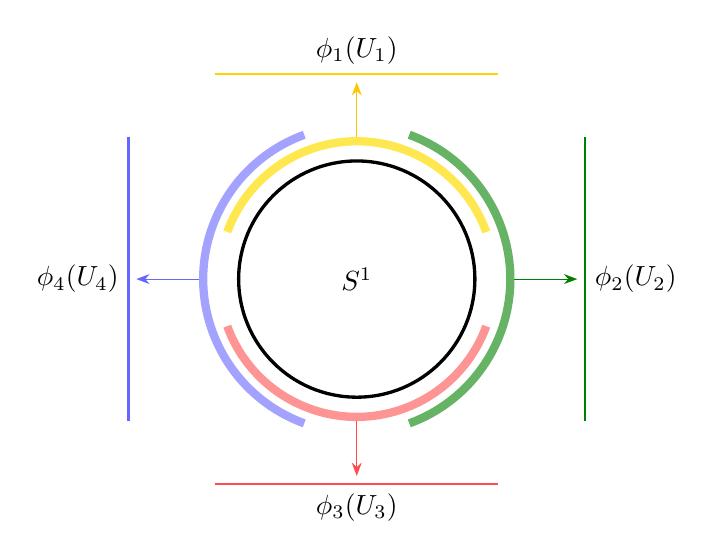
\begin{tikzpicture}[scale=1.0,>=Stealth]
  \draw[very thick] (0,0) circle (1.5);
  % top chart
  \draw[line width=3pt,yellow!80!orange,opacity=0.7] (20:1.75) arc (20:160:1.75);
  \draw[thick,yellow!70!orange] (-1.8,2.6) -- (1.8,2.6); \node[above] at (0,2.6) {$\phi_1(U_1)$};
  \draw[->,yellow!60!orange] (0,1.8) -- (0,2.5);
  % bottom
  \draw[line width=3pt,red!70,opacity=0.6] (200:1.75) arc (200:340:1.75);
  \draw[thick,red!70] (-1.8,-2.6) -- (1.8,-2.6); \node[below] at (0,-2.6) {$\phi_3(U_3)$};
  \draw[->,red!70] (0,-1.8) -- (0,-2.5);
  % left
  \draw[line width=3pt,blue!60,opacity=0.6] (110:1.95) arc (110:250:1.95);
  \draw[thick,blue!60] (-2.9,-1.8) -- (-2.9,1.8); \node[left] at (-2.9,0) {$\phi_4(U_4)$};
  \draw[->,blue!60] (-2.0,0) -- (-2.8,0);
  % right
  \draw[line width=3pt,green!50!black,opacity=0.6] (-70:1.95) arc (-70:70:1.95);
  \draw[thick,green!50!black] (2.9,-1.8) -- (2.9,1.8); \node[right] at (2.9,0) {$\phi_2(U_2)$};
  \draw[->,green!50!black] (2.0,0) -- (2.8,0);
  \node at (0,0) {$S^1$};
\end{tikzpicture}
\caption{An atlas for the circle $S^1$: four charts, each one mapping an open arc $U_i$ (coloured) onto an open interval of $\R$. No single chart can cover the whole circle (a homeomorphism from $S^1$ to an open interval does not exist), but together the four charts cover it; on the overlaps the transition maps are smooth.}
\label{fig:atlas}
\end{figure}

\begin{remarkbox}[What the definition is telling us]
Basically, we just found a definition that allows us to do calculus by mapping (pieces of) the manifold onto $\R^n$ and doing the differential calculus there. Given $p\in\M$ we map a neighbourhood of $p$ to $\R^n$, do ordinary tensor calculus, map back, move to a different neighbourhood, map again into $\R^n$, and so on. The mapping is \emph{local} and depends on the chart chosen; the compatibility condition guarantees that the results do not depend on which chart we use in the overlaps. \textbf{$\M$ locally looks like $\R^n$.}
\end{remarkbox}

\section{Scalars and curves}

\begin{definition}{Scalar field}{scalar}
A \textbf{scalar (field)} on space-time is a smooth map $S:\M\to\R$: to each point $p\in\M$ it associates a number $S(p)$.
\end{definition}
A scalar transforms ``trivially'' under coordinate transformations: its value at a given point is the same in all coordinates (every observer agrees on it),
\begin{equation}
  S'(x')=S(x)\qquad\text{under}\qquad x\to x'(x).
\end{equation}
The \emph{function} changes its form ($S'\neq S$ as functions of their arguments), but the \emph{number} attached to a given point does not.

\begin{definition}{Parametrised curve}{curve}
A \textbf{parametrised curve} on a manifold $\M$ is a smooth map $C:I\subseteq\R\to\M$, which to every real number $\lambda\in I$ associates a point $C(\lambda)\in\M$.
\end{definition}
If the image of $C$ lies inside a chart domain $U\subseteq\M$ with $\phi:U\to\R^n$, the composition
\begin{equation}
  \phi\circ C:\ I\subseteq\R\longrightarrow\R^n,\qquad \lambda\mapsto x^\mu(\lambda)\equiv\phi(C(\lambda))
\end{equation}
gives the \emph{coordinate functions} of the curve, on which we can do ordinary calculus (\cref{fig:curve}).

\begin{figure}[ht]
\centering
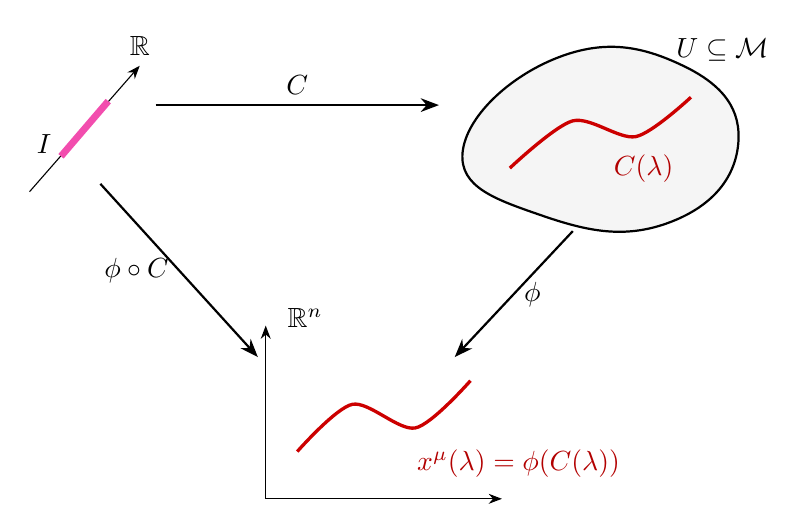
\begin{tikzpicture}[scale=1.0,>=Stealth]
  % interval
  \draw[->] (-0.5,1.7) -- (0.9,3.3) node[above] {$\R$};
  \draw[line width=2.5pt,magenta!70] (-0.1,2.15) -- (0.5,2.85);
  \node[left] at (-0.1,2.3) {$I$};
  % manifold
  \draw[thick,fill=gray!8] plot[smooth cycle,tension=0.8] coordinates {(5,2.2) (6.2,3.4) (7.8,3.3) (8.5,2.3) (7.6,1.3) (6,1.4)};
  \node at (8.3,3.5) {$U\subseteq\M$};
  \draw[very thick,red!80!black] plot[smooth] coordinates {(5.6,2.0) (6.4,2.6) (7.2,2.4) (7.9,2.9)};
  \node[red!70!black] at (7.3,2.0) {$C(\lambda)$};
  \draw[->,thick] (1.1,2.8) -- (4.7,2.8) node[midway,above] {$C$};
  % R^n
  \draw[->] (2.5,-2.2) -- (5.5,-2.2);
  \draw[->] (2.5,-2.2) -- (2.5,0.0);
  \node at (3.0,0.1) {$\R^n$};
  \draw[very thick,red!80!black] plot[smooth] coordinates {(2.9,-1.6) (3.6,-1.0) (4.4,-1.3) (5.1,-0.7)};
  \node[red!70!black,right] at (4.3,-1.75) {$x^\mu(\lambda)=\phi(C(\lambda))$};
  \draw[->,thick] (6.4,1.2) -- (4.9,-0.4) node[midway,right] {$\phi$};
  \draw[->,thick] (0.4,1.8) -- (2.4,-0.4) node[midway,left] {$\phi\circ C$};
\end{tikzpicture}
\caption{A parametrised curve $C:I\to\M$ and its coordinate representation $\phi\circ C:I\to\R^n$, obtained by composing with a chart $\phi$. Calculus is done in $\R^n$.}
\label{fig:curve}
\end{figure}

\section{Tangent vectors}

\paragraph{How do we differentiate along a curve?} Given a scalar $f$, its rate of change along $C$ is, by the chain rule,
\begin{equation}
  \frac{\dd}{\dd\lambda}f(C(\lambda))=\frac{\dd}{\dd\lambda}f(x^\mu(\lambda))=\frac{\dd x^\mu}{\dd\lambda}\frac{\pd f}{\pd x^\mu}.
\end{equation}
This holds for any $f$, so we have the identity of \emph{operators}
\begin{equation}
  \frac{\dd}{\dd\lambda}=\frac{\dd x^\mu}{\dd\lambda}\frac{\pd}{\pd x^\mu}=\frac{\dd x^\mu}{\dd\lambda}\pd_\mu .
\end{equation}
This defines a \textbf{vector}: the \emph{tangent vector} to the curve at $p$ is the operator
\begin{equation}
  \boxed{V\equiv\frac{\dd}{\dd\lambda}=\frac{\dd x^\mu}{\dd\lambda}\pd_\mu=V^\mu\pd_\mu,\qquad V^\mu\equiv\frac{\dd x^\mu}{\dd\lambda}.}
\end{equation}
The operator $V$ acts on any scalar field and returns its derivative along the curve; the numbers $V^\mu$ are its components.

\begin{definition}{Tangent space}{tangent-space}
Given $p\in\M$, let
\[
  C^\infty_{\M,p}\equiv\{C:(-\epsilon,\epsilon)\to\M\ |\ \epsilon>0,\ C\ \text{smooth},\ C(0)=p\}
\]
be the set of all smooth curves passing through $p$ at $\lambda=0$ (``smooth'' means that the coordinate functions $x^\mu(C(\lambda))$ can be differentiated as often as we like). The \textbf{tangent space} at $p$ is the set of their velocities:
\begin{equation}
  T_p(\M)=\{C'(0)\ |\ C\in C^\infty_{\M,p}\}.
\end{equation}
\end{definition}
For each curve through $p$ we compute its velocity at $p$ and collect them all in one set. Concretely, $C'(0)$ means:
\begin{itemize}[nosep]
  \item in a chart: the components $V^\mu=\left.\frac{\dd x^\mu(C(\lambda))}{\dd\lambda}\right|_{\lambda=0}$;
  \item as an operator on scalar fields: $C'(0)(f)=\left.\frac{\dd}{\dd\lambda}f(C(\lambda))\right|_{\lambda=0}$.
\end{itemize}
Strictly speaking, $C'(0)$ is an \emph{equivalence class} of curves: different curves can define the same vector. Two curves $C_1,C_2$ with $C_1(0)=C_2(0)=p$ are equivalent if
\begin{equation}
  \left.\frac{\dd}{\dd\lambda}x^\mu(C_1(\lambda))\right|_{\lambda=0}=\left.\frac{\dd}{\dd\lambda}x^\mu(C_2(\lambda))\right|_{\lambda=0}\qquad\forall\mu .
\end{equation}
The vector \emph{is} the class, and it is determined by the $n$ numbers $V^\mu$.

\begin{theorem}{Coordinate basis}{coord-basis}
$T_p(\M)$ is an $n$-dimensional vector space, and the partial derivatives $\{e_{(\mu)}\equiv\pd_\mu\}_{\mu=1,\dots,n}$ form a basis of it (the \emph{coordinate basis}).
\end{theorem}
\begin{proof}
\textbf{(1) Each $\pd_\mu$ is a tangent vector.} Take the coordinate line through $p$ along which only $x^\mu$ changes: $x^\alpha(\lambda)=x^\alpha_p+\lambda\,\delta^\alpha{}_\mu$. Its velocity at $p$ is $\dd x^\alpha/\dd\lambda=\delta^\alpha{}_\mu$. Acting on a scalar $f$:
\[
  \frac{\dd}{\dd\lambda}f=\frac{\dd x^\alpha}{\dd\lambda}\pd_\alpha f=\delta^\alpha{}_\mu\pd_\alpha f=\pd_\mu f .
\]
So the operator $\pd_\mu$ is exactly the tangent vector of the $\mu$-th coordinate line.

\textbf{(2) They span $T_p(\M)$.} Any tangent vector $V=\dd/\dd\lambda$ of some curve acts as $V(f)=\frac{\dd x^\mu}{\dd\lambda}\pd_\mu f=V^\mu\pd_\mu f$ for all $f$, hence $V=V^\mu\pd_\mu$: every vector is a linear combination of the $\pd_\mu$, with coefficients $V^\mu=\dd x^\mu/\dd\lambda$.

\textbf{(3) They are linearly independent.} Suppose $c^\mu\pd_\mu=0$ as an operator (the zero vector: $c^\mu\pd_\mu f=0$ for all $f$). Apply it to the coordinate function $f=x^\nu$ (which is a scalar field):
\[
  0=c^\mu\pd_\mu x^\nu=c^\mu\delta^\nu{}_\mu=c^\nu\qquad\forall\nu .
\]
So all $c^\nu=0$: no $\pd_\mu$ can be written in terms of the others.

Hence $\{\pd_\mu\}$ spans $T_p(\M)$ and is linearly independent: it is a basis, and $\dim T_p(\M)=n$.
\end{proof}

\subsection{Transformation law of vectors}

Under a coordinate change $x\to x'$, the chain rule gives for the components of the tangent vector
\begin{equation}
  V'^\mu=\frac{\dd x'^\mu}{\dd\lambda}=\frac{\pd x'^\mu}{\pd x^\nu}\frac{\dd x^\nu}{\dd\lambda}=\frac{\pd x'^\mu}{\pd x^\nu}V^\nu ,
\end{equation}
where $V^\nu$ are the components in the old coordinates and $V'^\mu$ those in the new ones.

\paragraph{Basis vectors transform the other way.} The object $V$ itself is coordinate independent: $V=V^\mu\pd_\mu=V'^\mu\pd'_\mu$. The chain rule gives
\begin{equation}
  \pd'_\mu=\frac{\pd}{\pd x'^\mu}=\frac{\pd x^\nu}{\pd x'^\mu}\frac{\pd}{\pd x^\nu}=\frac{\pd x^\nu}{\pd x'^\mu}\pd_\nu .
\end{equation}
Let us collect the relevant Jacobians:
\begin{equation}
  \Lambda^\mu{}_\nu\equiv\frac{\pd x'^\mu}{\pd x^\nu}\ \ \text{(Jacobian)},\qquad
  (\Lambda^{-1})^\mu{}_\nu=\frac{\pd x^\mu}{\pd x'^\nu}\ \ \text{(inverse)},
\end{equation}
and indeed, by the chain rule,
\begin{equation}
  \frac{\pd x'^\mu}{\pd x^\alpha}\frac{\pd x^\alpha}{\pd x'^\nu}=\frac{\pd x'^\mu}{\pd x'^\nu}=\delta^\mu{}_\nu,\qquad
  \frac{\pd x^\mu}{\pd x'^\alpha}\frac{\pd x'^\alpha}{\pd x^\nu}=\delta^\mu{}_\nu .
  \label{eq:jacobian-inverse}
\end{equation}
Using \eqref{eq:jacobian-inverse} we verify that the arrow is unchanged:
\begin{equation}
  V'^\mu\pd'_\mu=\frac{\pd x'^\mu}{\pd x^\alpha}V^\alpha\,\frac{\pd x^\nu}{\pd x'^\mu}\pd_\nu=\delta^\nu{}_\alpha V^\alpha\pd_\nu=V^\nu\pd_\nu=V .
\end{equation}

\begin{remarkbox}[Physical meaning]
Components and basis vectors transform in \emph{opposite} ways, so that the ``arrow'' itself is unchanged. If you stretch your basis vectors, the components shrink. This is the essence of the word ``contra-variant''.
\end{remarkbox}

\begin{definition}{Contravariant (tangent) vector}{vector}
A \textbf{contravariant} (or tangent) \textbf{vector} is an object $V$ whose components, under a general coordinate transformation $x\to x'$, transform as
\begin{equation}
  V'^\mu=\frac{\pd x'^\mu}{\pd x^\nu}V^\nu .
\end{equation}
\end{definition}
For a Lorentz transformation $\pd x'^\mu/\pd x^\nu=L^\mu{}_\nu$ and we recover \cref{ch:sr}.

\begin{example}{The displacement $\dd x^\mu$}{dx}
An example of contravariant vector is $\dd x^\mu$, since $\dd x'^\mu=\frac{\pd x'^\mu}{\pd x^\nu}\dd x^\nu$. We can derive this in two ways:
\begin{enumerate}[nosep]
\item take a tiny step along a curve $x^\mu(\lambda)$: the displacement is $\dd x^\mu=\frac{\dd x^\mu}{\dd\lambda}\dd\lambda=V^\mu\dd\lambda$, where $V^\mu$ are the components of the tangent vector and $\dd\lambda$ is just a number (a scalar, the same in all coordinates). So $\dd x^\mu$ transforms exactly like $V^\mu$;
\item directly, from the chain rule applied to $x'^\mu=x'^\mu(x)$: $\dd x'^\mu=\frac{\pd x'^\mu}{\pd x^\nu}\dd x^\nu$, which is the contravariant law with $V\to\dd x$.
\end{enumerate}
\end{example}

In summary, we can think of vectors as \textbf{first-order differential operators},
\begin{equation}
  V^\mu\ \longleftrightarrow\ V=V^\mu\pd_\mu,
\end{equation}
where $V^\mu$ are the components, $\pd_\mu$ the basis vectors, and $V$ the invariant object. In $\M$: $V\equiv\frac{\dd}{\dd\lambda}=V^\mu\pd_\mu\in T_p(\M)$.

\section{Covectors (one-forms)}

\begin{definition}{Covector}{covector}
A \textbf{covector} (or one-form) $U$ at $p$ is a \emph{linear} map $U:T_p(\M)\to\R$. Covectors form a vector space, the \textbf{cotangent space} $T_p^*(\M)$. Its \emph{dual basis} $\{\dd x^\mu\}$ is defined by
\begin{equation}
  \dd x^\mu(\pd_\nu)=\delta^\mu{}_\nu .
\end{equation}
Any covector can be expanded as $U=U_\mu\dd x^\mu$, and $U(V)=U_\mu V^\mu$.
\end{definition}

\paragraph{Explanation.}
\begin{enumerate}
  \item \emph{The dual basis picks components.} On a general vector $V=V^\nu\pd_\nu$, linearity gives
  \[
    \dd x^\mu(V)=\dd x^\mu(V^\nu\pd_\nu)=V^\nu\,\dd x^\mu(\pd_\nu)=V^\nu\delta^\mu{}_\nu=V^\mu :
  \]
  $\dd x^\mu$ picks out the $\mu$-th component of whatever vector it is fed.
  \item \emph{Action of an arbitrary covector.} $U$ is linear, so $U(V)=U(V^\nu\pd_\nu)=V^\nu U(\pd_\nu)$ for all $V$. Defining the $n$ numbers $U_\nu\equiv U(\pd_\nu)$ --- the \emph{components} of $U$ --- we get $U(V)=U_\nu V^\nu$.
  \item \emph{Why $U=U_\mu\dd x^\mu$.} Evaluate the proposed expansion on $V$: $(U_\mu\dd x^\mu)(V)=U_\mu\,\dd x^\mu(V)=U_\mu V^\mu$. This equals $U(V)$ for all $V$, so $U$ and $U_\mu\dd x^\mu$ are the same linear map. Hence $\{\dd x^\mu\}$ is a basis of $T_p^*(\M)$, and the components are $U_\mu=U(\pd_\mu)$.
\end{enumerate}

\paragraph{The differential of a function.} $\dd x^\mu$ is the differential of the coordinate function $x^\mu$. For any scalar $f$, the differential
\begin{equation}
  \dd f=\frac{\pd f}{\pd x^\mu}\dd x^\mu=(\pd_\mu f)\,\dd x^\mu
\end{equation}
is a covector with components $(\dd f)_\mu=\pd_\mu f$. Feeding it a vector gives the \emph{directional derivative}:
\begin{equation}
  \dd f(V)=(\pd_\mu f)V^\mu=(V^\mu\pd_\mu)(f)=V(f)=\frac{\dd f}{\dd\lambda}.
\end{equation}
Give it a direction $V$ and it returns how fast $f$ changes in that direction. Covectors are the objects that \emph{measure how much a scalar changes in a given direction}; the gradient $\pd_\mu f$ is the prime example, which is why it transforms as a covector.

\paragraph{Transformation law.} The number $U(V)$ cannot depend on the coordinates, so $U'_\mu V'^\mu=U_\alpha V^\alpha$. Inserting $V'^\mu=\frac{\pd x'^\mu}{\pd x^\alpha}V^\alpha$,
\[
  U'_\mu V'^\mu-U_\alpha V^\alpha=\left(U'_\mu\frac{\pd x'^\mu}{\pd x^\alpha}-U_\alpha\right)V^\alpha=0\qquad\forall V^\alpha
  \ \Longrightarrow\ U'_\mu\frac{\pd x'^\mu}{\pd x^\alpha}=U_\alpha .
\]
Multiplying by $\pd x^\alpha/\pd x'^\beta$ and using \eqref{eq:jacobian-inverse}, $U'_\mu\frac{\pd x'^\mu}{\pd x^\alpha}\frac{\pd x^\alpha}{\pd x'^\beta}=U'_\mu\delta^\mu{}_\beta=U'_\beta$, so
\begin{equation}
  U'_\beta=\frac{\pd x^\alpha}{\pd x'^\beta}U_\alpha .
\end{equation}

\begin{definition}{Covariant vector (covector)}{covector-law}
A \textbf{covector} is an object $U$ whose components transform under general coordinate transformations as
\begin{equation}
  U'_\mu=\frac{\pd x^\nu}{\pd x'^\mu}U_\nu .
\end{equation}
\end{definition}
\textit{Example:} the partial derivative (gradient) of a scalar $s$: $\left(\frac{\pd s}{\pd x^\mu}\right)'=\frac{\pd s}{\pd x'^\mu}=\frac{\pd x^\nu}{\pd x'^\mu}\frac{\pd s}{\pd x^\nu}$.

\section{General tensors}

\begin{definition}{Tensor of type $(p,q)$}{tensor}
A \textbf{tensor of type $(p,q)$} is an object with $p$ upper (contravariant) indices and $q$ lower (covariant) indices, whose components transform under $x\to x'$ with one Jacobian factor per index:
\begin{equation}
  T'^{\mu_1\dots\mu_p}{}_{\nu_1\dots\nu_q}=
  \frac{\pd x'^{\mu_1}}{\pd x^{\alpha_1}}\cdots\frac{\pd x'^{\mu_p}}{\pd x^{\alpha_p}}\,
  \frac{\pd x^{\beta_1}}{\pd x'^{\nu_1}}\cdots\frac{\pd x^{\beta_q}}{\pd x'^{\nu_q}}\,
  T^{\alpha_1\dots\alpha_p}{}_{\beta_1\dots\beta_q}.
  \label{eq:tensor-law}
\end{equation}
\end{definition}
Tensors transform \emph{linearly and homogeneously}: the new components are linear combinations of the old ones, with no additive term.

\begin{example}{Tensor product of two vectors}{tensor-product}
If $V,W$ are vectors (each a $(1,0)$ tensor), then
\[
  (V^\mu W^\nu)'=V'^\mu W'^\nu=\frac{\pd x'^\mu}{\pd x^\alpha}\frac{\pd x'^\nu}{\pd x^\beta}V^\alpha W^\beta ,
\]
which is the $(2,0)$ law: $V^\mu W^\nu$ are the components of the $(2,0)$ tensor $V\otimes W$.
\end{example}

\begin{proposition}{The Kronecker delta is a $(1,1)$ tensor}{delta}
The Kronecker delta $\delta^\mu{}_\nu$ is a $(1,1)$ tensor, and its components are $1$ or $0$ in every coordinate system.
\end{proposition}
\begin{proof}
Write $\delta^\mu{}_\nu=\pd x^\mu/\pd x^\nu$ and, in the primed system, $\delta'^\mu{}_\nu=\pd x'^\mu/\pd x'^\nu$ (the components of the identity in the primed system). Applying the chain rule through the unprimed coordinates:
\[
  \delta'^\mu{}_\nu=\frac{\pd x'^\mu}{\pd x'^\nu}=\frac{\pd x'^\mu}{\pd x^\alpha}\frac{\pd x^\alpha}{\pd x'^\nu}
  =\frac{\pd x'^\mu}{\pd x^\alpha}\frac{\pd x^\beta}{\pd x'^\nu}\delta^\alpha{}_\beta ,
\]
where in the last step we inserted $\delta^\alpha{}_\beta$ to rename the index $\alpha\to\beta$ in the second Jacobian. This is exactly the $(1,1)$ transformation law. Conversely, since $\delta^\alpha{}_\beta$ is $1$ when $\alpha=\beta$ and $0$ otherwise, the sum over $\beta$ keeps only $\beta=\alpha$: $\delta'^\mu{}_\nu=\frac{\pd x'^\mu}{\pd x^\alpha}\frac{\pd x^\alpha}{\pd x'^\nu}=\delta^\mu{}_\nu$ by \eqref{eq:jacobian-inverse}. Its components are $1$ or $0$ in every coordinate system.
\end{proof}

\section{Operations that produce tensors}

\begin{enumerate}[label=(\roman*)]
\item \textbf{Multiplication by a scalar:} if $T$ is a $(p,q)$ tensor and $a\in\R$, $aT$ is a $(p,q)$ tensor.
\item \textbf{Addition:} the sum of two tensors of the \emph{same} type $(p,q)$ is a $(p,q)$ tensor. \emph{You cannot add a $(1,0)$ and a $(0,1)$ tensor: they transform differently!}
\item \textbf{Tensor product:} $(p,q)\otimes(p',q')\to(p+p',q+q')$, e.g.\ $V^\mu W_\nu\equiv T^\mu{}_\nu$, i.e.\ $T=V\otimes W$.
\item \textbf{Contraction of indices:} set one upper and one lower index equal and sum: $(p,q)\to(p-1,q-1)$,
\[
  T^{\alpha_1\dots\alpha_k\dots\alpha_p}{}_{\beta_1\dots\beta_k\dots\beta_q}\ \longrightarrow\ T^{\alpha_1\dots\kappa\dots\alpha_p}{}_{\beta_1\dots\kappa\dots\beta_q}.
\]
Why does it work? For $T^\mu{}_\nu$:
\[
  T'^\mu{}_\mu=\frac{\pd x'^\mu}{\pd x^\alpha}\frac{\pd x^\beta}{\pd x'^\mu}T^\alpha{}_\beta=\delta^\beta{}_\alpha T^\alpha{}_\beta=T^\alpha{}_\alpha ,
\]
using \eqref{eq:jacobian-inverse}. The contracted object is a scalar (same value in every coordinate system). In particular $U_\mu V^\mu$ is a scalar. The same argument works for any pair of contracted indices in a general tensor: the two corresponding Jacobians combine into a $\delta$.
\item \textbf{Covariant differentiation} $D_\mu:(p,q)\to(p,q+1)$, introduced in \cref{ch:connection}. Let us see why it is needed: the ordinary derivative $\pd_\mu V^\nu$ of a vector is \emph{not} a tensor. Differentiating $V'^\nu=\frac{\pd x'^\nu}{\pd x^\beta}V^\beta$ --- both factors depend on the old coordinates $x^\alpha$, and $\frac{\pd}{\pd x'^\mu}=\frac{\pd x^\alpha}{\pd x'^\mu}\frac{\pd}{\pd x^\alpha}$ --- we get
\begin{equation}
  \pd'_\mu V'^\nu=\frac{\pd x^\alpha}{\pd x'^\mu}\frac{\pd}{\pd x^\alpha}\left(\frac{\pd x'^\nu}{\pd x^\beta}V^\beta\right)
  =\underbrace{\frac{\pd x^\alpha}{\pd x'^\mu}\frac{\pd x'^\nu}{\pd x^\beta}\pd_\alpha V^\beta}_{\text{(1) tensor law}}
  +\underbrace{\frac{\pd x^\alpha}{\pd x'^\mu}\frac{\pd^2x'^\nu}{\pd x^\alpha\pd x^\beta}V^\beta}_{\text{(2) inhomogeneous term}} .
  \label{eq:partial-not-tensor}
\end{equation}
The first term is the tensor law, while the second involves \emph{second derivatives} of the coordinate change, which vanish only for linear transformations (e.g.\ Lorentz). This extra term is what the connection $\Ga{\nu}{\mu}{\beta}$ in $D_\mu V^\nu=\pd_\mu V^\nu+\Ga{\nu}{\mu}{\beta}V^\beta$ will cancel.
\end{enumerate}

\begin{remarkbox}[Remarks]
\begin{itemize}
\item \textbf{If a tensor is zero in one coordinate system, it is zero in all coordinate systems.} Indeed $T'=(\text{Jacobian terms})\cdot T$ with no additive term, so $T=0\Rightarrow T'=0$. This is why tensor equations, such as the Einstein equations $G_{\mu\nu}=\frac{8\pi\GN}{c^4}T_{\mu\nu}$ (equivalently $G_{\mu\nu}-\frac{8\pi\GN}{c^4}T_{\mu\nu}=0$), valid in one coordinate system are true in all of them.
\item Keep track of which index belongs to which object: $V^\mu W^\nu=W^\nu V^\mu$ (the components are numbers), but $V^\mu W^\nu\neq V^\nu W^\mu$ in general.
\end{itemize}
\end{remarkbox}

\begin{definition}{Tensor field}{tensor-field}
A \textbf{scalar/vector/tensor field} is a smooth assignment of a scalar/vector/tensor to each point of the manifold.
\end{definition}

% =====================================================================
\chapter{The metric tensor}\label{ch:metric}
% =====================================================================

\section{Definition}

\begin{definition}{Metric tensor}{metric}
The \textbf{metric tensor} is a $(0,2)$ tensor field $g_{\mu\nu}(x)$ such that:
\begin{enumerate}[label=(\roman*),nosep]
  \item it is \textbf{symmetric}: $g_{\mu\nu}=g_{\nu\mu}$;
  \item it is \textbf{non-degenerate}: $\det(g_{\mu\nu})\neq0$;
  \item it defines the line element, which is invariant under general coordinate transformations $x\to x'$:
  \begin{equation}
    \dd s'^2=g'_{\mu\nu}(x')\dd x'^\mu\dd x'^\nu=g_{\mu\nu}(x)\dd x^\mu\dd x^\nu=\dd s^2\ (=c^2\dd\tau^2).
  \end{equation}
\end{enumerate}
\end{definition}
The metric describes the \emph{geometry} of the manifold: it defines lengths, angles, the scalar product of vectors ($g(V,W)=g_{\mu\nu}V^\mu W^\nu$) and proper time along world-lines. In GR the metric is the gravitational field itself. In SR, in inertial coordinates, $g_{\mu\nu}=\eta_{\mu\nu}$.

\begin{remarkbox}[Remark: the two meanings of $\dd x^\mu$]
The symbol $\dd x^\mu$ has two meanings, and it is worth being careful.
\begin{enumerate}
\item \textbf{Basis covector.} $\dd x^\mu$ is the covector (one-form) defined by $\dd x^\mu(\pd_\nu)=\delta^\mu{}_\nu$; it is part of the covector basis. For any vector $V=V^\mu\pd_\mu$ it extracts a component, $\dd x^\mu(V)=V^\mu$. Every covector is $U=U_\mu\dd x^\mu$, and $\dd f=\pd_\mu f\,\dd x^\mu$.
\item \textbf{Components of a small displacement.} Along a curve $x^\mu(\lambda)$, a step $\dd\lambda$ displaces the point by $\Delta=V\dd\lambda$ (tangent vector times a real number), whose components are
\[
  \Delta^\mu=\dd x^\mu(\Delta)=V^\mu\dd\lambda=\frac{\dd x^\mu}{\dd\lambda}\dd\lambda\equiv\dd x^\mu ,
\]
and these transform like vector components: $\dd x'^\mu=\frac{\pd x'^\mu}{\pd x^\nu}\dd x^\nu$.
\end{enumerate}
The notation is the same because the number in (2) is the output of the covector in (1) applied to the displacement. In $\dd s^2=g_{\mu\nu}\dd x^\mu\dd x^\nu$ the $\dd x^\mu$ are displacement components (meaning 2); in $g=g_{\mu\nu}\,\dd x^\mu\otimes\dd x^\nu$ they are basis covectors (meaning 1).
\end{remarkbox}

\section{Transformation law of the metric}

\begin{proposition}{The metric is a $(0,2)$ tensor}{metric-transf}
Requirement (iii) implies that the components of the metric transform as a $(0,2)$ tensor:
\begin{equation}
  g'_{\mu\nu}(x')=\frac{\pd x^\alpha}{\pd x'^\mu}\frac{\pd x^\beta}{\pd x'^\nu}\,g_{\alpha\beta}(x).
  \label{eq:metric-law}
\end{equation}
\end{proposition}
\begin{proof}
Notice first that, since $\dd x$ is a vector (from new to old coordinates, $x'\to x$),
\[
  \dd x^\alpha=\frac{\pd x^\alpha}{\pd x'^\mu}\dd x'^\mu,\qquad \dd x^\beta=\frac{\pd x^\beta}{\pd x'^\nu}\dd x'^\nu .
\]
Because $\dd s^2$ is a scalar,
\[
  g'_{\mu\nu}\dd x'^\mu\dd x'^\nu=g_{\alpha\beta}\dd x^\alpha\dd x^\beta=g_{\alpha\beta}\left(\frac{\pd x^\alpha}{\pd x'^\mu}\dd x'^\mu\right)\left(\frac{\pd x^\beta}{\pd x'^\nu}\dd x'^\nu\right).
\]
Rearranging,
\[
  \Big(\underbrace{g'_{\mu\nu}-\frac{\pd x^\alpha}{\pd x'^\mu}\frac{\pd x^\beta}{\pd x'^\nu}g_{\alpha\beta}}_{\equiv A_{\mu\nu}}\Big)\dd x'^\mu\dd x'^\nu=0\qquad\forall\,\dd x'^\mu .
\]
Now $A_{\mu\nu}$ is symmetric (it is built from the symmetric $g'_{\mu\nu}$ and $g_{\alpha\beta}$; exchanging $\mu\leftrightarrow\nu$ in the second term and relabelling $\alpha\leftrightarrow\beta$ gives back the same expression) and the displacement is arbitrary. We show that a symmetric array with $A_{\mu\nu}\xi^\mu\xi^\nu=0$ for all $\xi$ must vanish. Since $\dd x'^\mu\dd x'^\nu=\dd x'^\nu\dd x'^\mu$ (ordinary numbers), we can split the sum into diagonal and cross terms:
\[
  A_{\mu\nu}\dd x'^\mu\dd x'^\nu=\sum_\mu A_{\mu\mu}(\dd x'^\mu)^2+\sum_{\mu<\nu}(A_{\mu\nu}+A_{\nu\mu})\dd x'^\mu\dd x'^\nu=0 .
\]
We now choose the displacements to isolate each coefficient.
\begin{itemize}
\item Take a displacement with only the component $\ell$ non-zero. Then only one term survives: $A_{\ell\ell}(\dd x'^\ell)^2=0\Rightarrow A_{\ell\ell}=0$ (no sum on $\ell$).
\item Take a displacement with only the components $\ell$ and $\sigma$ non-zero ($\ell\neq\sigma$). The diagonal terms vanish by the previous point, so only the cross term remains: $(A_{\ell\sigma}+A_{\sigma\ell})\dd x'^\ell\dd x'^\sigma=0\Rightarrow A_{\ell\sigma}+A_{\sigma\ell}=0$.
\end{itemize}
Using the symmetry $A_{\sigma\ell}=A_{\ell\sigma}$, the last result gives $2A_{\ell\sigma}=0$. So every entry vanishes, $A_{\mu\nu}=0$, which is \eqref{eq:metric-law}.
\end{proof}

\section{The inverse metric}

From requirements (i) and (ii), $g_{\mu\nu}$ is an invertible matrix (invertibility actually only uses (ii)). We call its inverse $g^{\mu\nu}$:
\begin{equation}
  g_{\mu\nu}\,g^{\nu\alpha}=\delta_\mu{}^\alpha .
\end{equation}
$g^{\mu\nu}$ is also symmetric, because the inverse of a symmetric matrix is symmetric: $(g^{-1})^T=(g^T)^{-1}=g^{-1}$.

\begin{proposition}{The inverse metric is a $(2,0)$ tensor}{inv-metric}
\begin{equation}
  g'^{\mu\nu}=\frac{\pd x'^\mu}{\pd x^\alpha}\frac{\pd x'^\nu}{\pd x^\beta}\,g^{\alpha\beta}.
\end{equation}
\end{proposition}
\begin{proof}
Write $M^\alpha{}_\mu\equiv\pd x^\alpha/\pd x'^\mu$. The metric law reads, in matrix notation,
\[
  g'_{\mu\nu}=\sum_{\alpha,\beta}\frac{\pd x^\alpha}{\pd x'^\mu}\frac{\pd x^\beta}{\pd x'^\nu}g_{\alpha\beta}
  =\sum_{\alpha\beta}M^\alpha{}_\mu\,g_{\alpha\beta}\,M^\beta{}_\nu
  =\sum_{\alpha\beta}(M^T)_\mu{}^\alpha g_{\alpha\beta}M^\beta{}_\nu
  \quad\Longrightarrow\quad g'=M^TgM ,
\]
where we used that a matrix product $(XYZ)_{ij}=\sum X_{ik}Y_{k\ell}Z_{\ell j}$ chains indices from left to right, and rewrote $M^\alpha{}_\mu=(M^T)_\mu{}^\alpha$.
Taking the inverse of both sides, using $(XYZ)^{-1}=Z^{-1}Y^{-1}X^{-1}$ and $(M^T)^{-1}=(M^{-1})^T$,
\[
  (g')^{-1}=(M^TgM)^{-1}=M^{-1}g^{-1}(M^{-1})^T .
\]
The inverse of $M$ has entries $(M^{-1})^\mu{}_\alpha=\pd x'^\mu/\pd x^\alpha$, since $\frac{\pd x'^\mu}{\pd x^\alpha}\frac{\pd x^\alpha}{\pd x'^\nu}=\delta^\mu{}_\nu$. Back to indices,
\[
  g'^{\mu\nu}=(M^{-1})^\mu{}_\alpha\,g^{\alpha\beta}\,((M^{-1})^T)_\beta{}^\nu=(M^{-1})^\mu{}_\alpha\,g^{\alpha\beta}\,(M^{-1})^\nu{}_\beta
  =\frac{\pd x'^\mu}{\pd x^\alpha}\frac{\pd x'^\nu}{\pd x^\beta}g^{\alpha\beta},
\]
which is the $(2,0)$ tensor law.
\end{proof}

\section{Raising and lowering indices}

The metric tensor allows us to construct a vector from a covector and vice versa; in other words, it allows us to raise and lower indices:
\begin{equation}
  \boxed{U^\mu=g^{\mu\nu}U_\nu,\qquad U_\mu=g_{\mu\nu}U^\nu .}
\end{equation}

\paragraph{Geometric meaning.}
\begin{enumerate}[label=(\roman*)]
\item $g$ takes two vectors and returns a number: $g(V,W)=g_{\mu\nu}V^\mu W^\nu$.
\item Fix $V$ and leave the second slot open: $W\mapsto g(V,W)=g_{\mu\nu}V^\mu W^\nu$. This map eats one vector $W$ and returns a number, and it is linear in $W$ (because $g$ is bilinear): by definition, it is a covector. Call it $U$: $U(W)\equiv g(V,W)$.
\item Its components are $U_\nu=U(\pd_\nu)$. The components of the basis vector $\pd_\nu$ are $W^\alpha=\delta^\alpha{}_\nu$, so
\[
  U_\nu=U(\pd_\nu)=g(V,\pd_\nu)=g_{\mu\alpha}V^\mu\delta^\alpha{}_\nu=g_{\mu\nu}V^\mu\ \Longrightarrow\ \boxed{V_\nu=g_{\nu\mu}V^\mu} .
\]
\end{enumerate}
The inverse operation is consistent: from $V_\nu=g_{\nu\mu}V^\mu$, $g^{\alpha\nu}V_\nu=g^{\alpha\nu}g_{\nu\mu}V^\mu=\delta^\alpha{}_\mu V^\mu=V^\alpha$; and $g_{\mu\nu}g^{\nu\alpha}U_\alpha=\delta_\mu{}^\alpha U_\alpha=U_\mu$.

\paragraph{Raising and lowering produce tensors,} because they are a tensor product followed by a contraction. Let us check explicitly that $U_\mu=g_{\mu\nu}U^\nu$ transforms as a lower index. With $M^\alpha{}_\mu=\pd x^\alpha/\pd x'^\mu$ and $N^\nu{}_\gamma=\pd x'^\nu/\pd x^\gamma$ (so that $M^\beta{}_\nu N^\nu{}_\gamma=\delta^\beta{}_\gamma$):
\[
  U'_\mu=g'_{\mu\nu}U'^\nu=\big(M^\alpha{}_\mu M^\beta{}_\nu g_{\alpha\beta}\big)\big(N^\nu{}_\gamma U^\gamma\big)
  =M^\alpha{}_\mu g_{\alpha\beta}\delta^\beta{}_\gamma U^\gamma=M^\alpha{}_\mu g_{\alpha\gamma}U^\gamma=M^\alpha{}_\mu U_\alpha ,
\]
which is the $(0,1)$ law: $U'_\mu=\frac{\pd x^\alpha}{\pd x'^\mu}U_\alpha$. The same works for any index of any tensor, e.g.\ $T^\mu{}_\nu=g_{\nu\alpha}T^{\mu\alpha}$.

\begin{example}{Minkowski space}{mink-lower}
With $(+,-,-,-)$: $V_\mu=\eta_{\mu\nu}V^\nu=(V^0,-\vec V)$. For instance $p_\mu=(E/c,-\vec p)$ and $\dd s^2=\dd x_\mu\dd x^\mu$. In Minkowski space spatial indices are raised and lowered with $-\delta_{ij}$: $V_i=-V^i$.
\end{example}

\begin{remarkbox}[Remark: the trace $\delta^\mu{}_\mu$]
$g_{\mu\nu}g^{\mu\nu}=\delta^\mu{}_\mu=n$, the dimension of the manifold ($=4$ in space-time). This identity is used repeatedly (e.g.\ when taking traces of the Einstein equations).
\end{remarkbox}

% =====================================================================
\chapter{Parallel transport, connection and geodesics}\label{ch:connection}
% =====================================================================

\section{The problem: comparing vectors at different points}

In the plane $\R^2$, to compare two vectors $\vec u$ and $\vec v$ attached at different points, we simply translate $\vec v$ parallel to itself until it sits at the same point as $\vec u$, and then compare them (\cref{fig:pt-flat}, left). The result does not depend on the path along which we translate $\vec v$.

On a curved space, e.g.\ the surface of a sphere, all vectors are tangent to the surface, and the natural notion of ``moving a vector parallel to itself'' (keeping it tangent and not rotating it) gives a result that \emph{depends on the path} (\cref{fig:pt-flat}, right): this is the \textbf{problem} we have to address. To formulate it we need a notion of derivative of vector fields that makes sense on a manifold.

\begin{figure}[ht]
\centering
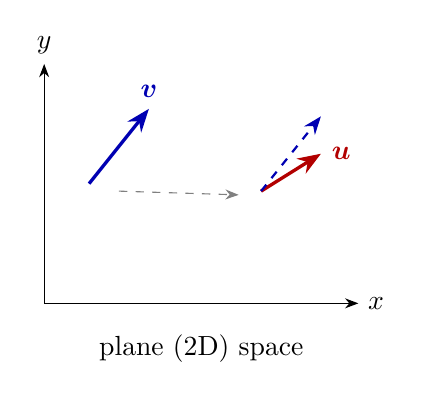
\begin{tikzpicture}[scale=0.95,>=Stealth]
  \draw[->] (0,0) -- (4.2,0) node[right] {$x$};
  \draw[->] (0,0) -- (0,3.2) node[above] {$y$};
  \draw[->,very thick,blue!70!black] (0.6,1.6) -- (1.4,2.6) node[above] {$\vec v$};
  \draw[->,very thick,red!70!black] (2.9,1.5) -- (3.7,2.0) node[right] {$\vec u$};
  \draw[->,thick,blue!70!black,dashed] (2.9,1.5) -- (3.7,2.5);
  \draw[->,gray,dashed] (1.0,1.5) -- (2.6,1.45);
  \node at (2.1,-0.6) {plane (2D) space};
\end{tikzpicture}
\hspace{1.2cm}
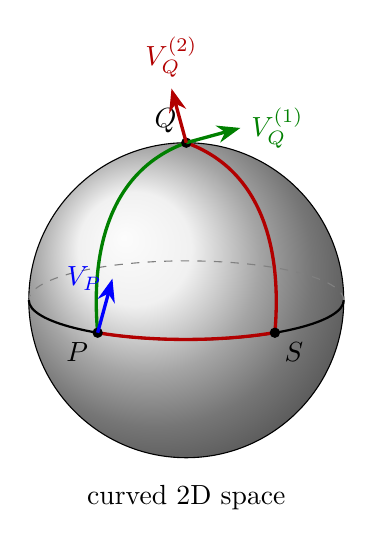
\begin{tikzpicture}[scale=1.25,>=Stealth]
  \shade[ball color=gray!15] (0,0) circle (1.6);
  \draw (0,0) circle (1.6);
  \draw[dashed,gray] (1.6,0) arc (0:180:1.6 and 0.4);
  \draw[thick] (-1.6,0) arc (180:360:1.6 and 0.4);
  % points
  \coordinate (Q) at (0,1.6);
  \coordinate (P) at (-0.9,-0.33);
  \coordinate (S) at (0.9,-0.33);
  % path 1: P -> Q along meridian
  \draw[very thick,green!50!black] (P) to[out=95,in=200] (Q);
  % path 2: P -> S along equator then S -> Q
  \draw[very thick,red!70!black] (P) arc (236:304:1.6 and 0.4);
  \draw[very thick,red!70!black] (S) to[out=85,in=-20] (Q);
  \fill (P) circle (1.5pt) node[below left] {$P$};
  \fill (Q) circle (1.5pt) node[above left] {$Q$};
  \fill (S) circle (1.5pt) node[below right] {$S$};
  % vectors
  \draw[->,very thick,blue] (P) -- ++(0.15,0.55) node[left] {$V_P$};
  \draw[->,very thick,green!50!black] (Q) -- ++(0.55,0.15) node[right] {$V_Q^{(1)}$};
  \draw[->,very thick,red!70!black] (Q) -- ++(-0.15,0.55) node[above] {$V_Q^{(2)}$};
  \node at (0,-2.0) {curved 2D space};
\end{tikzpicture}
\caption{Left: in flat space a vector $\vec v$ can be translated parallel to itself to the point of $\vec u$ and compared with it, independently of the path. Right: on a sphere, transporting the tangent vector $V_P$ ``parallel to itself'' from $P$ to $Q$ along path (1) (green) or along path (2) (red, first along the equator to $S$, then up a meridian) gives different vectors at $Q$: the final orientation depends on the path.}
\label{fig:pt-flat}
\end{figure}

\paragraph{First attempt: partial derivatives.} Is the partial derivative of a vector a tensor? Take a vector $A^\nu$ and ask whether $\pd_\mu A^\nu\equiv\pd A^\nu/\pd x^\mu$ is a $(1,1)$ tensor. Under a general coordinate transformation, with $\pd'_\mu=\frac{\pd x^\alpha}{\pd x'^\mu}\pd_\alpha$ and $A'^\nu=\frac{\pd x'^\nu}{\pd x^\beta}A^\beta$, we already found in \eqref{eq:partial-not-tensor}:
\begin{equation}
  (\pd_\mu A^\nu)'=\underbrace{\frac{\pd x^\alpha}{\pd x'^\mu}\frac{\pd x'^\nu}{\pd x^\beta}\pd_\alpha A^\beta}_{\text{tensor-like}}
  +\underbrace{\frac{\pd x^\alpha}{\pd x'^\mu}\frac{\pd^2x'^\nu}{\pd x^\alpha\pd x^\beta}A^\beta}_{\text{not tensor-like}} .
\end{equation}
$\pd_\mu A^\nu$ is \textbf{not} a tensor (epic fail!). The physical reason is clear: $\pd_\mu A^\nu$ compares the components of $A$ at two neighbouring points, $A^\nu(x+\dd x)-A^\nu(x)$, but the two vectors live in different tangent spaces, and the components are taken with respect to bases that themselves change from point to point.

\section{Interlude: locally inertial (Riemann normal) coordinates}

\begin{theorem}{Riemann normal coordinates}{rnc}
For every metric $g_{\mu\nu}$ it is possible to find coordinates $x'$ (\emph{Riemann normal coordinates}, or locally inertial coordinates) such that, at \emph{one} chosen point $P$ (with $x_P=0=x'_P$):
\begin{enumerate}[nosep]
  \item $g'_{\mu\nu}(x'_P)=\eta_{\mu\nu}$;
  \item $\pd'_\rho g'_{\mu\nu}\big|_{x'_P}=0$;
  \item but in general $\pd'_\rho\pd'_\sigma g'_{\mu\nu}\big|_{x'_P}\neq0$, unless the space is flat.
\end{enumerate}
\end{theorem}
\begin{proofsketch}
Expand the coordinate transformation around $P$: $x^\mu=\frac{\pd x^\mu}{\pd x'^\alpha}\big|_P x'^\alpha+\frac12\frac{\pd^2x^\mu}{\pd x'^\alpha\pd x'^\beta}\big|_P x'^\alpha x'^\beta+\frac16\frac{\pd^3 x^\mu}{\pd x'^\alpha\pd x'^\beta\pd x'^\gamma}\big|_P x'^\alpha x'^\beta x'^\gamma+\dots$ and use $g'_{\mu\nu}=\frac{\pd x^\alpha}{\pd x'^\mu}\frac{\pd x^\beta}{\pd x'^\nu}g_{\alpha\beta}$. Count the free parameters order by order (in 4D):
\begin{itemize}[nosep]
\item order 0: the $4\times4=16$ numbers $\pd x^\mu/\pd x'^\alpha|_P$ can be used to set the $10$ components of $g'_{\mu\nu}(P)$ to $\eta_{\mu\nu}$ (any symmetric non-degenerate matrix of signature $(+,-,-,-)$ can be brought to $\eta$); the $6$ remaining parameters are the Lorentz transformations, which preserve $\eta$;
\item order 1: the $4\times10=40$ numbers $\pd^2x^\mu/\pd x'^\alpha\pd x'^\beta|_P$ (symmetric in $\alpha\beta$) can be used to cancel the $10\times4=40$ first derivatives $\pd'_\rho g'_{\mu\nu}(P)$;
\item order 2: the $4\times20=80$ third derivatives (symmetric in three indices) are not enough to cancel the $10\times10=100$ second derivatives $\pd'_\rho\pd'_\sigma g'_{\mu\nu}(P)$: $100-80=20$ combinations survive. These are precisely the $20$ independent components of the Riemann tensor (\cref{ch:curvature}), which measures the curvature.
\end{itemize}
\end{proofsketch}
This is the mathematical expression of the Equivalence Principle: at any point, a freely-falling observer can choose coordinates in which, locally (to first order), space-time looks like Minkowski space-time and gravity is absent; curvature (tidal effects) shows up at second order.

\section{The covariant derivative}

We define the \textbf{covariant derivative} of a vector field $A^\nu$ as
\begin{equation}
  \boxed{D_\mu A^\nu\equiv\pd_\mu A^\nu+\Ga{\nu}{\mu}{\lambda}A^\lambda}
  \label{eq:cov-der-vector}
\end{equation}
and \emph{require} that it transforms as a $(1,1)$ tensor. The first term tells us ``how much the vector changes'', the second ``how much the coordinates (basis) change''. The coefficients $\Ga{\nu}{\mu}{\lambda}$ are called \textbf{Christoffel symbols} or \textbf{affine connection coefficients}.

\begin{proposition}{The $\Gamma$'s are not tensors}{gamma-transf}
For $D_\mu V^\nu$ to be a $(1,1)$ tensor, the connection coefficients must transform as
\begin{equation}
  \Gamma'^{\alpha}{}_{\beta\rho}=
  \underbrace{\frac{\pd x'^\alpha}{\pd x^\nu}\frac{\pd x^\mu}{\pd x'^\beta}\frac{\pd x^\lambda}{\pd x'^\rho}\Ga{\nu}{\mu}{\lambda}}_{\text{tensor-like}}
  -\underbrace{\frac{\pd x^\mu}{\pd x'^\beta}\frac{\pd x^\lambda}{\pd x'^\rho}\frac{\pd^2x'^\alpha}{\pd x^\mu\pd x^\lambda}}_{\text{inhomogeneous}} .
  \label{eq:gamma-transf}
\end{equation}
Because of the inhomogeneous term, the $\Gamma$'s are \textbf{not} tensors.
\end{proposition}
\begin{proof}
Useful relations: (i) $V'^\alpha=\frac{\pd x'^\alpha}{\pd x^\nu}V^\nu\Leftrightarrow V^\nu=\frac{\pd x^\nu}{\pd x'^\alpha}V'^\alpha$; (ii) for covectors $V'_\mu=\frac{\pd x^\alpha}{\pd x'^\mu}V_\alpha$; (iii) for a $(1,1)$ tensor $T'^\alpha{}_\beta=\frac{\pd x'^\alpha}{\pd x^\nu}\frac{\pd x^\mu}{\pd x'^\beta}T^\nu{}_\mu$.

We demand $(D_\beta V^\alpha)'=\frac{\pd x'^\alpha}{\pd x^\nu}\frac{\pd x^\mu}{\pd x'^\beta}D_\mu V^\nu$, i.e.
\[
  \pd'_\beta V'^\alpha+\Gamma'^\alpha{}_{\beta\rho}V'^\rho
  =\frac{\pd x'^\alpha}{\pd x^\nu}\frac{\pd x^\mu}{\pd x'^\beta}\left(\pd_\mu V^\nu+\Ga{\nu}{\mu}{\lambda}V^\lambda\right).
\]
Using \eqref{eq:partial-not-tensor} for the first term on the left and $V'^\rho=\frac{\pd x'^\rho}{\pd x^\lambda}V^\lambda$ for the second,
\[
  \frac{\pd x^\mu}{\pd x'^\beta}\frac{\pd x'^\alpha}{\pd x^\nu}\pd_\mu V^\nu
  +\frac{\pd x^\mu}{\pd x'^\beta}\frac{\pd^2x'^\alpha}{\pd x^\mu\pd x^\lambda}V^\lambda
  +\Gamma'^\alpha{}_{\beta\rho}\frac{\pd x'^\rho}{\pd x^\lambda}V^\lambda
  =\frac{\pd x'^\alpha}{\pd x^\nu}\frac{\pd x^\mu}{\pd x'^\beta}\pd_\mu V^\nu+\frac{\pd x'^\alpha}{\pd x^\nu}\frac{\pd x^\mu}{\pd x'^\beta}\Ga{\nu}{\mu}{\lambda}V^\lambda .
\]
The terms with $\pd_\mu V^\nu$ cancel. The remaining equation must hold for all $V^\lambda$:
\[
  \Gamma'^\alpha{}_{\beta\rho}\frac{\pd x'^\rho}{\pd x^\lambda}
  =\frac{\pd x'^\alpha}{\pd x^\nu}\frac{\pd x^\mu}{\pd x'^\beta}\Ga{\nu}{\mu}{\lambda}-\frac{\pd x^\mu}{\pd x'^\beta}\frac{\pd^2x'^\alpha}{\pd x^\mu\pd x^\lambda}.
\]
Multiplying both sides by $\pd x^\lambda/\pd x'^\sigma$ and using $\frac{\pd x'^\rho}{\pd x^\lambda}\frac{\pd x^\lambda}{\pd x'^\sigma}=\delta^\rho{}_\sigma$ gives \eqref{eq:gamma-transf} (with $\sigma$ renamed $\rho$).
\end{proof}

\paragraph{Torsion.} Although $\Gamma$ is not a tensor, the \emph{difference of two connections} is, because the inhomogeneous terms cancel. In particular, consider $\Ga{\mu}{\nu}{\lambda}$ and $\tilde\Gamma^\mu{}_{\nu\lambda}\equiv\Ga{\mu}{\lambda}{\nu}$ (indices swapped). Then the \textbf{torsion}
\begin{equation}
  T^\mu{}_{\nu\lambda}\equiv\Ga{\mu}{\nu}{\lambda}-\Ga{\mu}{\lambda}{\nu}
\end{equation}
is a $(1,2)$ tensor. \textit{Proof:} applying \eqref{eq:gamma-transf} to both terms,
\[
  T'^\alpha{}_{\beta\rho}=\frac{\pd x'^\alpha}{\pd x^\nu}\frac{\pd x^\mu}{\pd x'^\beta}\frac{\pd x^\lambda}{\pd x'^\rho}\left(\Ga{\nu}{\mu}{\lambda}-\Ga{\nu}{\lambda}{\mu}\right)
  -\frac{\pd x^\mu}{\pd x'^\beta}\frac{\pd x^\lambda}{\pd x'^\rho}\left(\frac{\pd^2x'^\alpha}{\pd x^\mu\pd x^\lambda}-\frac{\pd^2x'^\alpha}{\pd x^\lambda\pd x^\mu}\right),
\]
(in the second term we renamed the dummy indices $\mu\leftrightarrow\lambda$). The last bracket vanishes because partial derivatives commute, so $T'^\alpha{}_{\beta\rho}=\frac{\pd x'^\alpha}{\pd x^\nu}\frac{\pd x^\mu}{\pd x'^\beta}\frac{\pd x^\lambda}{\pd x'^\rho}T^\nu{}_{\mu\lambda}$. $\blacksquare$

\begin{keyresult}
General Relativity is a \textbf{torsion-free} theory: $T^\mu{}_{\nu\lambda}=0$, i.e.\ $\Ga{\mu}{\nu}{\lambda}=\Ga{\mu}{\lambda}{\nu}$ (the connection is symmetric in its lower indices). Since $T$ is a tensor, this statement is coordinate independent.
\end{keyresult}

\paragraph{Covariant derivative along a vector field.} Given a vector field $A$, the covariant derivative of $V$ along $A$ is
\begin{equation}
  D_AV^\mu\equiv A^\nu D_\nu V^\mu .
\end{equation}

\subsection{Covariant derivative of general tensors}

\begin{definition}{Covariant derivative}{covder}
The covariant derivative of tensors is an operation such that:
\begin{enumerate}[nosep]
\item $D_\mu$ is a linear operator mapping $(p,q)$ tensors to $(p,q+1)$ tensors;
\item acting on scalars it reduces to the partial derivative: $D_\mu S=\pd_\mu S$;
\item it obeys the Leibniz rule:
$D_\mu\big(A^{\mu_1\dots\mu_p}{}_{\nu_1\dots\nu_q}B^{\rho_1\dots\rho_r}{}_{\lambda_1\dots\lambda_s}\big)
=(D_\mu A^{\dots}{}_{\dots})B^{\dots}{}_{\dots}+A^{\dots}{}_{\dots}(D_\mu B^{\dots}{}_{\dots})$.
\end{enumerate}
\end{definition}

\begin{example}{Covariant derivative of a covector}{covder-covector}
$U_\nu V^\nu$ is a scalar, so by 2) and 3):
\begin{align*}
  D_\mu(U_\nu V^\nu)&=\pd_\mu(U_\nu V^\nu)=(\pd_\mu U_\nu)V^\nu+U_\nu\pd_\mu V^\nu ,\\
  D_\mu(U_\nu V^\nu)&=(D_\mu U_\nu)V^\nu+U_\nu D_\mu V^\nu=(D_\mu U_\nu)V^\nu+U_\nu\pd_\mu V^\nu+U_\nu\Ga{\nu}{\mu}{\lambda}V^\lambda .
\end{align*}
Equating, $(D_\mu U_\nu)V^\nu=(\pd_\mu U_\nu)V^\nu-U_\lambda\Ga{\lambda}{\mu}{\nu}V^\nu$ (renaming $\nu\leftrightarrow\lambda$ in the last term). Since $V$ is arbitrary,
\begin{equation}
  \boxed{D_\mu U_\nu=\pd_\mu U_\nu-\Ga{\lambda}{\mu}{\nu}U_\lambda .}
\end{equation}
\end{example}
In the general case, there is a $+\Gamma$ term for each upper index and a $-\Gamma$ term for each lower index:
\begin{align}
  D_\mu T^{\nu_1\dots\nu_p}{}_{\rho_1\dots\rho_q}=\pd_\mu T^{\nu_1\dots\nu_p}{}_{\rho_1\dots\rho_q}
  &+\Ga{\nu_1}{\mu}{\lambda}T^{\lambda\nu_2\dots\nu_p}{}_{\rho_1\dots\rho_q}+\dots+\Ga{\nu_p}{\mu}{\lambda}T^{\nu_1\dots\nu_{p-1}\lambda}{}_{\rho_1\dots\rho_q}\nonumber\\
  &-\Ga{\lambda}{\mu}{\rho_1}T^{\nu_1\dots\nu_p}{}_{\lambda\rho_2\dots\rho_q}-\dots-\Ga{\lambda}{\mu}{\rho_q}T^{\nu_1\dots\nu_p}{}_{\rho_1\dots\rho_{q-1}\lambda}.
\end{align}

\subsection{Properties and the Christoffel symbols}

In GR the connection is chosen such that:
\begin{enumerate}[nosep]
\item $D_\mu$ commutes with index contraction;
\item \textbf{metric compatibility}: $\boxed{D_\alpha g_{\mu\nu}=0}$;
\item consequently, $D_\mu$ commutes with raising and lowering of indices ($D_\mu V_\nu=D_\mu(g_{\nu\alpha}V^\alpha)=g_{\nu\alpha}D_\mu V^\alpha$);
\item covariant derivatives commute on scalars, $D_\mu D_\nu S=D_\nu D_\mu S$ (equivalent to torsion-freeness: $D_\mu D_\nu S-D_\nu D_\mu S=-T^\lambda{}_{\mu\nu}\pd_\lambda S$).
\end{enumerate}
\begin{remarkbox}[Why $D_\alpha g_{\mu\nu}=0$?]
In Riemann normal coordinates at $P$, $\pd g=0$ and (as we will see) $\Gamma=0$, so $D_\alpha g_{\mu\nu}=\pd_\alpha g_{\mu\nu}=0$ at $P$. Since $D_\alpha g_{\mu\nu}$ is a tensor, it vanishes at $P$ in every coordinate system; and $P$ is arbitrary. Physically: in a local inertial frame the metric is locally constant (Equivalence Principle).
\end{remarkbox}

\begin{theorem}{Levi-Civita connection (Christoffel symbols)}{christoffel}
The unique torsion-free, metric-compatible connection is
\begin{equation}
  \boxed{\Ga{\lambda}{\sigma}{\rho}=\frac12 g^{\lambda\mu}\left(\pd_\sigma g_{\rho\mu}+\pd_\rho g_{\sigma\mu}-\pd_\mu g_{\sigma\rho}\right).}
  \label{eq:christoffel}
\end{equation}
Equivalently, lowering the index, $\Gamma_{\mu\sigma\rho}\equiv g_{\mu\lambda}\Ga{\lambda}{\sigma}{\rho}=\frac12(\pd_\sigma g_{\rho\mu}+\pd_\rho g_{\sigma\mu}-\pd_\mu g_{\sigma\rho})$.
\end{theorem}
\begin{proof}
Write metric compatibility, $D_\rho g_{\sigma\mu}=\pd_\rho g_{\sigma\mu}-\Ga{\lambda}{\rho}{\sigma}g_{\lambda\mu}-\Ga{\lambda}{\rho}{\mu}g_{\sigma\lambda}=0$, for three cyclic permutations of the indices:
\begin{align*}
  \text{(a)}\quad &\pd_\rho g_{\sigma\mu}-\Ga{\lambda}{\rho}{\sigma}g_{\lambda\mu}-\Ga{\lambda}{\rho}{\mu}g_{\sigma\lambda}=0,\\
  \text{(b)}\quad &\pd_\sigma g_{\mu\rho}-\Ga{\lambda}{\sigma}{\mu}g_{\lambda\rho}-\Ga{\lambda}{\sigma}{\rho}g_{\mu\lambda}=0,\\
  \text{(c)}\quad &\pd_\mu g_{\rho\sigma}-\Ga{\lambda}{\mu}{\rho}g_{\lambda\sigma}-\Ga{\lambda}{\mu}{\sigma}g_{\rho\lambda}=0.
\end{align*}
Compute (a)$+$(b)$-$(c), using $g_{\mu\nu}=g_{\nu\mu}$ and the symmetry $\Ga{\lambda}{\rho}{\sigma}=\Ga{\lambda}{\sigma}{\rho}$:
the terms $\Ga{\lambda}{\rho}{\mu}g_{\sigma\lambda}$ (from (a)) and $\Ga{\lambda}{\mu}{\rho}g_{\lambda\sigma}$ (from (c)) cancel; the terms $\Ga{\lambda}{\sigma}{\mu}g_{\lambda\rho}$ (from (b)) and $\Ga{\lambda}{\mu}{\sigma}g_{\rho\lambda}$ (from (c)) cancel; the terms $\Ga{\lambda}{\rho}{\sigma}g_{\lambda\mu}$ and $\Ga{\lambda}{\sigma}{\rho}g_{\mu\lambda}$ add up. We get
\[
  \pd_\rho g_{\sigma\mu}+\pd_\sigma g_{\mu\rho}-\pd_\mu g_{\rho\sigma}-2\Ga{\lambda}{\sigma}{\rho}g_{\lambda\mu}=0 .
\]
Multiplying by $\frac12 g^{\mu\kappa}$ and using $g_{\lambda\mu}g^{\mu\kappa}=\delta_\lambda{}^\kappa$ gives \eqref{eq:christoffel} (with $\kappa$ renamed $\lambda$). The derivation shows uniqueness: $\Gamma$ is completely determined by $g$.
\end{proof}

\begin{remarkbox}[Counting]
In 4D a general connection has $4^3=64$ components. Symmetry in the lower indices removes the $4\times6=24$ antisymmetric combinations, leaving $64-24=40$ independent $\Gamma$'s --- exactly the $40$ first derivatives $\pd_\rho g_{\mu\nu}$ ($4\times10$), consistent with \eqref{eq:christoffel} being an invertible linear relation between them. In Riemann normal coordinates $\pd g=0$ at $P$, hence $\Gamma(P)=0$: \emph{one can always make the Christoffel symbols vanish at a point}, but not, in general, in a neighbourhood.
\end{remarkbox}

\paragraph{Geometric meaning of the $\Gamma$'s.} Consider a vector $\vec V=V^\alpha\vec e_{(\alpha)}$ expanded on basis vectors which change from point to point. Then
\[
  \frac{\pd\vec V}{\pd x^\beta}=\frac{\pd V^\alpha}{\pd x^\beta}\vec e_{(\alpha)}+V^\alpha\frac{\pd\vec e_{(\alpha)}}{\pd x^\beta}.
\]
Writing the derivative of the basis vectors in the same basis, $\frac{\pd\vec e_{(\alpha)}}{\pd x^\beta}=\Ga{\mu}{\alpha}{\beta}\vec e_{(\mu)}$, we find $\frac{\pd\vec V}{\pd x^\beta}=\big(\pd_\beta V^\mu+\Ga{\mu}{\beta}{\alpha}V^\alpha\big)\vec e_{(\mu)}=(D_\beta V^\mu)\,\vec e_{(\mu)}$. Hence: \emph{$\Ga{\mu}{\alpha}{\beta}$ is the $\mu$-th component of the derivative of the $\alpha$-th basis vector with respect to the $\beta$-th coordinate}, and $D_\beta V^\mu$ are the components of the full derivative of the geometric object $\vec V$.

\section{Parallel transport}

\begin{definition}{Parallel transport}{pt}
Let $C:[a,b]\subseteq\R\to U\subseteq\M$ be a parametrised curve which, in a given coordinate system, reads $x^\mu(\lambda)$, $\lambda\in\R$. A vector $V$ is \textbf{parallel transported} along the curve if and only if
\begin{equation}
  \frac{DV^\mu}{\dd\lambda}\equiv\frac{\dd x^\nu}{\dd\lambda}D_\nu V^\mu=\frac{\dd V^\mu}{\dd\lambda}+\Ga{\mu}{\nu}{\lambda}\frac{\dd x^\nu}{\dd\lambda}V^\lambda=0
\end{equation}
everywhere along the curve (``covariant derivative along the curve'').
\end{definition}
Here $\dd x^\nu/\dd\lambda$ is the tangent vector (the ``velocity'') to the curve. The second form follows from $\frac{\dd x^\nu}{\dd\lambda}\pd_\nu V^\mu=\frac{\dd V^\mu}{\dd\lambda}$. Given $V$ at one point, this is a first-order ODE which determines $V$ uniquely along the curve.

\begin{remarkbox}[Properties]
\begin{itemize}[nosep]
\item Since $D_\alpha g_{\mu\nu}=0$, if $V$ and $W$ are both parallel transported then
$\frac{\dd}{\dd\lambda}(g_{\mu\nu}V^\mu W^\nu)=\frac{\dd x^\alpha}{\dd\lambda}D_\alpha(g_{\mu\nu}V^\mu W^\nu)=0$. Parallel transport preserves the \textbf{scalar product}, hence the \textbf{norm} of vectors (length is invariant under PT) and the \textbf{angles} between them.
\item The \textbf{covariant acceleration} of a curve is defined as
\begin{equation}
  a^\mu\equiv\frac{D\dot x^\mu}{\dd\lambda}=\ddot x^\mu+\Ga{\mu}{\nu}{\lambda}\dot x^\nu\dot x^\lambda=\dot x^\nu D_\nu\dot x^\mu,\qquad \dot x^\mu\equiv\frac{\dd x^\mu}{\dd\lambda}.
\end{equation}
\end{itemize}
\end{remarkbox}

\section{Geodesics}

\begin{definition}{Geodesic}{geodesic}
Let $V^\mu(x)=\frac{\dd x^\mu}{\dd\lambda}$ be the tangent vector field to a curve $C(\lambda)$. $C$ is a \textbf{geodesic} if and only if its tangent vector is parallel transported along itself:
\begin{equation}
  \boxed{\frac{\dd^2x^\mu}{\dd\lambda^2}+\Ga{\mu}{\nu}{\rho}\frac{\dd x^\nu}{\dd\lambda}\frac{\dd x^\rho}{\dd\lambda}=0}\qquad\text{(geodesic equation)}.
  \label{eq:geodesic}
\end{equation}
\end{definition}
\paragraph{Comments.}
\begin{enumerate}
\item The geodesic equation defines a curve such that, if a vector is tangent to $C(\lambda)$ at one point, it stays tangent at all points along $C$ (``auto-parallel'' curve). A geodesic is a curve of \emph{zero covariant acceleration}: it is what would have been a straight path in a flat space.
\item The geodesic equations retain their form under all \emph{affine} reparametrisations, $\lambda\to\tilde\lambda=a\lambda+b$ ($a,b$ constants): then $\dd/\dd\lambda=a\,\dd/\dd\tilde\lambda$ and each term of \eqref{eq:geodesic} gets multiplied by $a^2$. Such parameters are called \emph{affine parameters} (for massive particles, e.g.\ the proper time $\tau$).
\item The covariant acceleration vanishes along affinely parametrised geodesics, $a^\mu=\frac{D\dot x^\mu}{\dd\lambda}=\frac{\dd^2x^\mu}{\dd\lambda^2}+\Ga{\mu}{\nu}{\rho}\frac{\dd x^\nu}{\dd\lambda}\frac{\dd x^\rho}{\dd\lambda}=0$.
\item There is one geodesic equation for each component $\mu$: a system of $n$ coupled second-order ODEs.
\end{enumerate}

\subsection{Geodesics extremise the proper time}

Why are geodesics physically relevant? Consider the proper time, $c^2\dd\tau^2=\dd s^2=g_{\mu\nu}\dd x^\mu\dd x^\nu$, elapsed between two events $A$ and $B$ along a time-like world-line:
\begin{equation}
  \tau_{AB}=\int_A^B\dd\tau=\int_A^B\sqrt{g_{\mu\nu}\dd x^\mu\dd x^\nu}
\end{equation}
(we set $c=1$ in this subsection). For simplicity, take a world-line parametrised as $x^\alpha=x^\alpha(\sigma)$ with $\sigma=0$ at $A$ and $\sigma=1$ at $B$:
\[
  \tau_{AB}=\int_0^1\left[g_{\alpha\beta}\frac{\dd x^\alpha}{\dd\sigma}\frac{\dd x^\beta}{\dd\sigma}\right]^{1/2}\dd\sigma\equiv\int_0^1 L\!\left[\frac{\dd x^\alpha}{\dd\sigma},x^\alpha\right]\dd\sigma ,
  \qquad L\equiv\left[g_{\alpha\beta}\frac{\dd x^\alpha}{\dd\sigma}\frac{\dd x^\beta}{\dd\sigma}\right]^{1/2}=\frac{\dd\tau}{\dd\sigma}.
\]
A useful relation: for any function $F=F(\tau(\sigma))$,
\begin{equation}
  \frac{\dd F}{\dd\sigma}=\frac{\dd F}{\dd\tau}\frac{\dd\tau}{\dd\sigma}=L\frac{\dd F}{\dd\tau}.\tag{$\ast$}
\end{equation}
From analytical mechanics, the action is extremised when $L$ obeys the Euler--Lagrange equations,
\[
  \frac{\pd L}{\pd x^\gamma}-\frac{\dd}{\dd\sigma}\left[\frac{\pd L}{\pd(\dd x^\gamma/\dd\sigma)}\right]=0 .
\]
Let us compute each term.
\begin{itemize}
\item \textbf{First term.} Only the metric depends on $x^\gamma$:
\[
  \frac{\pd L}{\pd x^\gamma}=\frac{1}{2L}\frac{\pd g_{\alpha\beta}}{\pd x^\gamma}\frac{\dd x^\alpha}{\dd\sigma}\frac{\dd x^\beta}{\dd\sigma}
  \overset{(\ast)}{=}\frac{L}{2}\frac{\pd g_{\alpha\beta}}{\pd x^\gamma}\frac{\dd x^\alpha}{\dd\tau}\frac{\dd x^\beta}{\dd\tau}.
\]
\item \textbf{Second term.} Using $\pd(\dd x^\alpha/\dd\sigma)/\pd(\dd x^\gamma/\dd\sigma)=\delta^\alpha{}_\gamma$,
\[
  \frac{\pd L}{\pd(\dd x^\gamma/\dd\sigma)}=\frac{1}{2L}g_{\alpha\beta}\left(\delta^\alpha{}_\gamma\frac{\dd x^\beta}{\dd\sigma}+\frac{\dd x^\alpha}{\dd\sigma}\delta^\beta{}_\gamma\right)
  =\frac{1}{2L}\left(g_{\gamma\beta}\frac{\dd x^\beta}{\dd\sigma}+g_{\alpha\gamma}\frac{\dd x^\alpha}{\dd\sigma}\right)=\frac1L g_{\alpha\gamma}\frac{\dd x^\alpha}{\dd\sigma},
\]
since the two terms are equal (dummy indices, symmetric metric). By $(\ast)$, $\frac1L\frac{\dd x^\alpha}{\dd\sigma}=\frac{\dd x^\alpha}{\dd\tau}$, and
\begin{align*}
  \frac{\dd}{\dd\sigma}\left[\frac{\pd L}{\pd(\dd x^\gamma/\dd\sigma)}\right]
  &=\frac{\dd}{\dd\sigma}\left[g_{\alpha\gamma}\frac{\dd x^\alpha}{\dd\tau}\right]\overset{(\ast)}{=}L\frac{\dd}{\dd\tau}\left[g_{\alpha\gamma}\frac{\dd x^\alpha}{\dd\tau}\right]
  =L\left[g_{\alpha\gamma}\frac{\dd^2x^\alpha}{\dd\tau^2}+\frac{\dd g_{\alpha\gamma}}{\dd\tau}\frac{\dd x^\alpha}{\dd\tau}\right]\\
  &=L\left[g_{\alpha\gamma}\frac{\dd^2x^\alpha}{\dd\tau^2}+\frac{\pd g_{\alpha\gamma}}{\pd x^\beta}\frac{\dd x^\beta}{\dd\tau}\frac{\dd x^\alpha}{\dd\tau}\right]
  =L\left[g_{\alpha\gamma}\frac{\dd^2x^\alpha}{\dd\tau^2}+\frac12\left(\frac{\pd g_{\alpha\gamma}}{\pd x^\beta}+\frac{\pd g_{\beta\gamma}}{\pd x^\alpha}\right)\frac{\dd x^\alpha}{\dd\tau}\frac{\dd x^\beta}{\dd\tau}\right],
\end{align*}
where in the last step we split the term into two equal halves and relabelled $\alpha\leftrightarrow\beta$ in one of them.
\end{itemize}
Putting the pieces together and dividing by $L$:
\[
  \frac12\frac{\pd g_{\alpha\beta}}{\pd x^\gamma}\frac{\dd x^\alpha}{\dd\tau}\frac{\dd x^\beta}{\dd\tau}-g_{\alpha\gamma}\frac{\dd^2x^\alpha}{\dd\tau^2}-\frac12\left(\frac{\pd g_{\alpha\gamma}}{\pd x^\beta}+\frac{\pd g_{\beta\gamma}}{\pd x^\alpha}\right)\frac{\dd x^\alpha}{\dd\tau}\frac{\dd x^\beta}{\dd\tau}=0,
\]
that is
\[
  g_{\alpha\gamma}\frac{\dd^2x^\alpha}{\dd\tau^2}=-\frac12\left[\pd_\beta g_{\gamma\alpha}+\pd_\alpha g_{\gamma\beta}-\pd_\gamma g_{\alpha\beta}\right]\frac{\dd x^\alpha}{\dd\tau}\frac{\dd x^\beta}{\dd\tau}
  =-g_{\gamma\lambda}\Ga{\lambda}{\alpha}{\beta}\frac{\dd x^\alpha}{\dd\tau}\frac{\dd x^\beta}{\dd\tau},
\]
by \eqref{eq:christoffel}. Multiplying by $g^{\gamma\mu}$:
\begin{equation}
  \frac{\dd^2x^\mu}{\dd\tau^2}+\Ga{\mu}{\alpha}{\beta}\frac{\dd x^\alpha}{\dd\tau}\frac{\dd x^\beta}{\dd\tau}=0 .
\end{equation}

\begin{keyresult}
The geodesic equation is the equation of the curve along which the action (the proper time) is \emph{extremised}. Free particles --- both massive and massless --- follow geodesics. (For massless particles $\dd\tau=0$ and one uses an affine parameter $\lambda$ and the Lagrangian below.)
\end{keyresult}

\begin{proposition}{The ``squared'' Lagrangian}{L1}
The function $L_1\equiv\frac12L^2=\frac12 g_{\mu\nu}\dot x^\mu\dot x^\nu$ (with $\dot{}=\dd/\dd\lambda$, $\lambda$ an affine parameter) also obeys the Euler--Lagrange equations and gives the geodesic equation.
\end{proposition}
\begin{proof}
$\pd L_1/\pd\dot x^\gamma=L\,\pd L/\pd\dot x^\gamma$ and $\pd L_1/\pd x^\gamma=L\,\pd L/\pd x^\gamma$. Then
\[
\frac{\dd}{\dd\lambda}\frac{\pd L_1}{\pd\dot x^\gamma}-\frac{\pd L_1}{\pd x^\gamma}=L\left[\frac{\dd}{\dd\lambda}\frac{\pd L}{\pd\dot x^\gamma}-\frac{\pd L}{\pd x^\gamma}\right]+\frac{\dd L}{\dd\lambda}\frac{\pd L}{\pd\dot x^\gamma}.
\]
For an affine parameter $L=\dd\tau/\dd\lambda$ is constant, so the last term vanishes and the two sets of equations are equivalent. Directly: $\frac{\dd}{\dd\lambda}(g_{\gamma\mu}\dot x^\mu)-\frac12\pd_\gamma g_{\mu\nu}\dot x^\mu\dot x^\nu=0$ reproduces, as above, $\ddot x^\mu+\Ga{\mu}{\alpha}{\beta}\dot x^\alpha\dot x^\beta=0$. This version has the advantage of avoiding square roots and of being valid also for null geodesics.
\end{proof}

\subsection{Example: geodesics of the Euclidean plane in polar coordinates}

Consider the 2D Euclidean space. We look for its geodesics, in Cartesian and in polar coordinates. The line element is
\[
  \dd s^2=\dd x^2+\dd y^2=\dd r^2+r^2\dd\phi^2,
\]
so the components of $g$ are
\[
  g_{xx}=g_{yy}=1,\ g_{xy}=g_{yx}=0;\qquad g_{rr}=1,\ g_{\phi\phi}=r^2,\ g_{r\phi}=g_{\phi r}=0 .
\]
\begin{enumerate}[label=(\roman*)]
\item \textbf{Cartesian:} $g_{\mu\nu}=\delta_{\mu\nu}$, so all partial derivatives of the metric vanish and all $\Gamma=0$. The geodesic equations are $\frac{\dd^2x}{\dd\lambda^2}=0$, $\frac{\dd^2y}{\dd\lambda^2}=0$, with general solution $x(\lambda)=a\lambda+b$, $y(\lambda)=c\lambda+d$, i.e.\ $y=kx+e$: a \textbf{straight line}. (In flat space-time one usually parametrises with the proper time, $\tau=t$ for a particle at rest.)
\item \textbf{Polar:} the only non-vanishing derivative is $\pd_r g_{\phi\phi}=2r$. From \eqref{eq:christoffel}:
\[
  \Ga{r}{\phi}{\phi}=\frac12 g^{rr}(-\pd_r g_{\phi\phi})=-r,\qquad
  \Ga{\phi}{r}{\phi}=\Ga{\phi}{\phi}{r}=\frac12 g^{\phi\phi}\pd_r g_{\phi\phi}=\frac{1}{2r^2}2r=\frac1r ,
\]
all others vanish. The geodesic equations are
\begin{align}
  \frac{\dd^2r}{\dd\lambda^2}+\Ga{r}{\phi}{\phi}\left(\frac{\dd\phi}{\dd\lambda}\right)^2=0&\quad\Longrightarrow\quad\ddot r-r\dot\phi^2=0,\\
  \frac{\dd^2\phi}{\dd\lambda^2}+2\Ga{\phi}{r}{\phi}\frac{\dd r}{\dd\lambda}\frac{\dd\phi}{\dd\lambda}=0&\quad\Longrightarrow\quad\ddot\phi+\frac2r\dot r\dot\phi=0,
\end{align}
where the factor $2$ comes from the two terms $\Ga{\phi}{r}{\phi}\dot r\dot\phi+\Ga{\phi}{\phi}{r}\dot\phi\dot r$ (symmetric lower indices).
\end{enumerate}
These are also straight lines --- the physics remains the same when changing coordinates --- even though in polar coordinates the Christoffel symbols are non-zero: \emph{even in flat space there can be non-zero Christoffel symbols}. Choosing coordinate systems wisely is important!

\textit{Check with the Lagrangian method.} With $L_1=\frac12(\dot r^2+r^2\dot\phi^2)$: $\frac{\dd}{\dd\lambda}\dot r-r\dot\phi^2=0$ and $\frac{\dd}{\dd\lambda}(r^2\dot\phi)=0\Leftrightarrow r^2\ddot\phi+2r\dot r\dot\phi=0$: the same equations. The second one expresses conservation of angular momentum $r^2\dot\phi$. One can verify that $r\cos(\phi-\phi_0)=\text{const}$ (a straight line at distance $|\text{const}|$ from the origin) solves them.

% =====================================================================
\chapter{Curvature}\label{ch:curvature}
% =====================================================================

We want to study curvature in an \emph{intrinsic} way, i.e.\ using only quantities defined on the manifold itself (the metric and the connection), without reference to any higher-dimensional space in which the manifold might be embedded. This is the \textbf{intrinsic curvature}.

\section{Intrinsic versus extrinsic curvature: why is a cylinder flat?}

A cylinder looks curved when seen from the three-dimensional space in which it is embedded (it has \emph{extrinsic} curvature). But for a two-dimensional being living on its surface it is flat. Take a rectangular sheet of paper (\cref{fig:cylinder}): starting from a point $P$, going straight forward and turning by $90^\circ$ four times we come back to the \emph{same} initial point, as in the plane. The sheet can be rolled into a cylinder \emph{without stretching or tearing it} (without adding defects): distances and angles measured on the surface are unchanged, so a cylinder is \textbf{flat} from the geometric (intrinsic) point of view. On the contrary, it is impossible to wrap a sheet of paper around a sphere without adding defects (creases or tears): the sphere is intrinsically curved. On a sphere, a ``square'' made of four geodesic segments with four right angles does not close (and a triangle made of geodesics has a sum of angles larger than $\pi$).

\begin{figure}[ht]
\centering
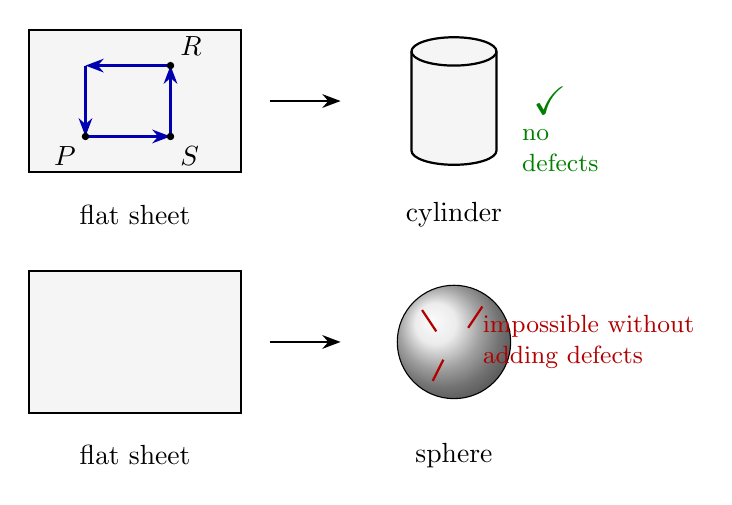
\begin{tikzpicture}[scale=0.9,>=Stealth]
  % sheet with closed path
  \draw[thick,fill=gray!8] (0,0) rectangle (3,2);
  \draw[->,thick,blue!70!black] (0.8,0.5) -- (2.0,0.5);
  \draw[->,thick,blue!70!black] (2.0,0.5) -- (2.0,1.5);
  \draw[->,thick,blue!70!black] (2.0,1.5) -- (0.8,1.5);
  \draw[->,thick,blue!70!black] (0.8,1.5) -- (0.8,0.5);
  \fill (0.8,0.5) circle (1.5pt) node[below left] {$P$};
  \fill (2.0,0.5) circle (1.5pt) node[below right] {$S$};
  \fill (2.0,1.5) circle (1.5pt) node[above right] {$R$};
  \node at (1.5,-0.6) {flat sheet};
  % to cylinder
  \draw[->,thick] (3.4,1) -- (4.4,1);
  \begin{scope}[shift={(5.4,0)}]
    \draw[thick,fill=gray!8] (0,0.3) -- (0,1.7) arc (180:0:0.6 and 0.2) -- (1.2,0.3) arc (0:-180:0.6 and 0.2);
    \draw[thick] (0,1.7) arc (180:360:0.6 and 0.2);
    \node at (0.6,-0.6) {cylinder};
    \node[green!50!black] at (1.95,1) {\Large\checkmark};
    \node[green!50!black,align=left,font=\small] at (2.1,0.3) {no\\defects};
  \end{scope}
  % to sphere
  \begin{scope}[shift={(0,-3.4)}]
    \draw[thick,fill=gray!8] (0,0) rectangle (3,2);
    \node at (1.5,-0.6) {flat sheet};
    \draw[->,thick] (3.4,1) -- (4.4,1);
    \shade[ball color=gray!20] (6.0,1) circle (0.8);
    \draw (6.0,1) circle (0.8);
    \draw[red!70!black,thick] (5.55,1.45) -- (5.75,1.15) (6.4,1.5) -- (6.2,1.2) (5.7,0.45) -- (5.85,0.75);
    \node at (6.0,-0.6) {sphere};
    \node[red!70!black,align=left,font=\small] at (7.9,1) {impossible without\\adding defects};
  \end{scope}
\end{tikzpicture}
\caption{A flat sheet can be rolled into a cylinder without any distortion: the cylinder is intrinsically flat (a closed ``square'' path $P\to S\to R\to\dots\to P$ made of straight segments and right angles still closes). A sheet cannot be wrapped on a sphere without creasing or tearing it: the sphere is intrinsically curved.}
\label{fig:cylinder}
\end{figure}

The idea we will now make precise is: \emph{curvature is the failure of a vector to come back to itself when parallel transported around a closed loop}, or equivalently the dependence of parallel transport on the path (\cref{fig:pt-flat}).

\section{The Riemann tensor from parallel transport}

Consider a small coordinate ``rectangle'' on the manifold, delimited by coordinate lines of $x^1$ and $x^2$ (all other coordinates fixed), with corners (\cref{fig:loop})
\[
  P=(x^1,x^2),\quad Q=(x^1+\delta x^1,x^2),\quad R=(x^1+\delta x^1,x^2+\delta x^2),\quad S=(x^1,x^2+\delta x^2).
\]
\textbf{Goal:} parallel transport a tangent vector $V$ from $P$ to $R$ along the two paths $C:P\to Q\to R$ and $C':P\to S\to R$, and compare the results.

\begin{figure}[ht]
\centering
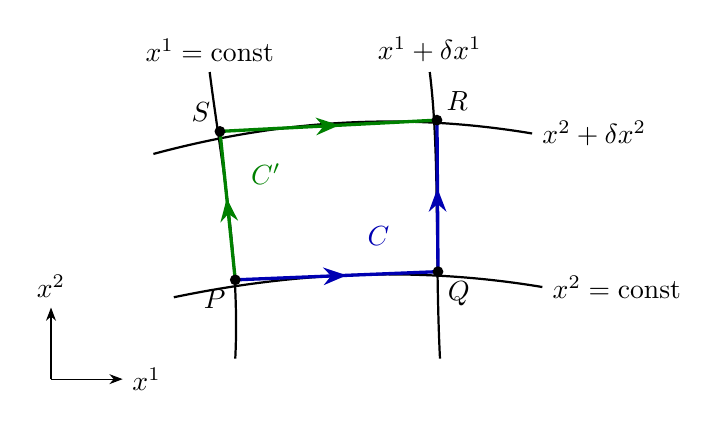
\begin{tikzpicture}[scale=1.3,>=Stealth]
  \draw[thick] (0,0) .. controls (1.2,0.25) and (2.4,0.3) .. (3.6,0.1) node[right] {$x^2=\text{const}$};
  \draw[thick] (-0.2,1.4) .. controls (1.1,1.75) and (2.3,1.8) .. (3.5,1.6) node[right] {$x^2+\delta x^2$};
  \draw[thick] (0.6,-0.6) .. controls (0.65,0.4) and (0.45,1.4) .. (0.35,2.2) node[above] {$x^1=\text{const}$};
  \draw[thick] (2.6,-0.6) .. controls (2.55,0.4) and (2.6,1.4) .. (2.5,2.2) node[above] {$x^1+\delta x^1$};
  \coordinate (P) at (0.6,0.17);
  \coordinate (Q) at (2.58,0.25);
  \coordinate (R) at (2.57,1.73);
  \coordinate (S) at (0.45,1.62);
  \draw[->,very thick,blue!70!black] (P) -- ($(P)!0.55!(Q)$);
  \draw[very thick,blue!70!black] ($(P)!0.5!(Q)$) -- (Q);
  \draw[->,very thick,blue!70!black] (Q) -- ($(Q)!0.55!(R)$);
  \draw[very thick,blue!70!black] ($(Q)!0.5!(R)$) -- (R);
  \draw[->,very thick,green!50!black] (P) -- ($(P)!0.55!(S)$);
  \draw[very thick,green!50!black] ($(P)!0.5!(S)$) -- (S);
  \draw[->,very thick,green!50!black] (S) -- ($(S)!0.55!(R)$);
  \draw[very thick,green!50!black] ($(S)!0.5!(R)$) -- (R);
  \foreach \p/\pos in {P/below left,Q/below right,R/above right,S/above left} \fill (\p) circle (1.5pt) node[\pos] {$\p$};
  \node[blue!70!black] at (2.0,0.6) {$C$};
  \node[green!50!black] at (0.9,1.2) {$C'$};
  \draw[->] (-1.2,-0.8) -- (-0.5,-0.8) node[right] {$x^1$};
  \draw[->] (-1.2,-0.8) -- (-1.2,-0.1) node[above] {$x^2$};
\end{tikzpicture}
\caption{Parallel transport of a vector from $P$ to $R$ along the path $C:P\to Q\to R$ (blue) and along the path $C':P\to S\to R$ (green), on a small coordinate loop of sides $\delta x^1$ and $\delta x^2$.}
\label{fig:loop}
\end{figure}

\paragraph{Reminders.} $D_\nu V^\mu=\pd_\nu V^\mu+\Ga{\mu}{\nu}{\lambda}V^\lambda$ and parallel transport: $\frac{\dd x^\nu}{\dd\lambda}D_\nu V^\mu=0$.

\paragraph{(i) Transport $P\to Q$:} only $x^1$ changes, so $\dd x^2/\dd\lambda=0$ and
\begin{gather*}
  \frac{\dd x^\nu}{\dd\lambda}D_\nu V^\mu=\frac{\dd x^1}{\dd\lambda}D_1V^\mu=0\ \Longrightarrow\ \frac{\dd x^1}{\dd\lambda}\big[\pd_1V^\mu+\Ga{\mu}{1}{\lambda}V^\lambda\big]_{x^2}=0\\
  \Longrightarrow\quad \boxed{\pd_1V^\mu\big|_{x^2}=-\Ga{\mu}{1}{\lambda}V^\lambda\big|_{x^2}}\quad\text{(result A)}.
\end{gather*}
Integrating from $x^1$ to $x^1+\delta x^1$ (the left-hand side gives the variation of $V$ as we move from $P$ to $Q$):
\begin{equation}
  V_C^\mu(Q)=V^\mu(P)-\underbrace{\int_{x^1}^{x^1+\delta x^1}\Ga{\mu}{1}{\lambda}V^\lambda\,\dd x^1\Big|_{x^2}}_{\equiv I_1}.
\end{equation}
\paragraph{(ii) Transport $Q\to R$:} only $x^2$ changes; in the same way ($\pd_2V^\mu=-\Ga{\mu}{2}{\lambda}V^\lambda$),
\begin{equation}
  V_C^\mu(R)=V_C^\mu(Q)-\underbrace{\int_{x^2}^{x^2+\delta x^2}\Ga{\mu}{2}{\lambda}V^\lambda\,\dd x^2\Big|_{x^1+\delta x^1}}_{\equiv I_2}.
\end{equation}
\paragraph{(iii) Transport $P\to S$:}
\begin{equation}
  V_{C'}^\mu(S)=V^\mu(P)-\underbrace{\int_{x^2}^{x^2+\delta x^2}\Ga{\mu}{2}{\lambda}V^\lambda\,\dd x^2\Big|_{x^1}}_{\equiv I_3}.
\end{equation}
\paragraph{(iv) Transport $S\to R$:}
\begin{equation}
  V_{C'}^\mu(R)=V_{C'}^\mu(S)-\underbrace{\int_{x^1}^{x^1+\delta x^1}\Ga{\mu}{1}{\lambda}V^\lambda\,\dd x^1\Big|_{x^2+\delta x^2}}_{\equiv I_4}.
\end{equation}

\paragraph{The difference.}
\begin{align}
  V_C^\mu(R)-V_{C'}^\mu(R)&=\big[V^\mu(P)-I_1-I_2\big]-\big[V^\mu(P)-I_3-I_4\big]=(I_4-I_1)+(I_3-I_2)\nonumber\\
  &=\underbrace{\int_{x^1}^{x^1+\delta x^1}\Big[\Ga{\mu}{1}{\lambda}V^\lambda\big|_{x^2+\delta x^2}-\Ga{\mu}{1}{\lambda}V^\lambda\big|_{x^2}\Big]\dd x^1}_{\equiv I_{41}}\nonumber\\
  &\quad+\underbrace{\int_{x^2}^{x^2+\delta x^2}\Big[\Ga{\mu}{2}{\lambda}V^\lambda\big|_{x^1}-\Ga{\mu}{2}{\lambda}V^\lambda\big|_{x^1+\delta x^1}\Big]\dd x^2}_{\equiv I_{32}} .
\end{align}
For small $\delta x^{1,2}$ we Taylor-expand the integrands, keeping only first-order terms:
\begin{align*}
  \Ga{\mu}{1}{\lambda}V^\lambda\big|_{x^2+\delta x^2}&\simeq\Ga{\mu}{1}{\lambda}V^\lambda\big|_{x^2}+\Big[\pd_2\big(\Ga{\mu}{1}{\lambda}V^\lambda\big)\Big]_{x^2}\delta x^2 \quad\text{(expansion in $x^2$)},\\
  \Ga{\mu}{2}{\lambda}V^\lambda\big|_{x^1+\delta x^1}&\simeq\Ga{\mu}{2}{\lambda}V^\lambda\big|_{x^1}+\Big[\pd_1\big(\Ga{\mu}{2}{\lambda}V^\lambda\big)\Big]_{x^1}\delta x^1 \quad\text{(expansion in $x^1$)}.
\end{align*}
Hence
\[
  I_{41}\simeq\delta x^2\int_{x^1}^{x^1+\delta x^1}\pd_2\big(\Ga{\mu}{1}{\lambda}V^\lambda\big)\dd x^1,\qquad
  I_{32}\simeq-\delta x^1\int_{x^2}^{x^2+\delta x^2}\pd_1\big(\Ga{\mu}{2}{\lambda}V^\lambda\big)\dd x^2 .
\]
To the same (second) order in the small displacements we can treat the integrands as constant over the (small) integration interval:
\[
  I_{41}\simeq\delta x^1\delta x^2\,\pd_2\big(\Ga{\mu}{1}{\lambda}V^\lambda\big),\qquad I_{32}\simeq-\delta x^1\delta x^2\,\pd_1\big(\Ga{\mu}{2}{\lambda}V^\lambda\big).
\]
Now we open the derivatives and use result A (and its analogue $\pd_2V^\lambda=-\Ga{\lambda}{2}{\alpha}V^\alpha$), which tells us how $V$ varies along the parallel-transport path:
\begin{align*}
  I_{41}&\simeq\delta x^1\delta x^2\big[(\pd_2\Ga{\mu}{1}{\lambda})V^\lambda+\Ga{\mu}{1}{\lambda}\pd_2V^\lambda\big]
  =\delta x^1\delta x^2\big[(\pd_2\Ga{\mu}{1}{\lambda})V^\lambda-\Ga{\mu}{1}{\lambda}\Ga{\lambda}{2}{\alpha}V^\alpha\big]\\
  &=\delta x^1\delta x^2\big(\pd_2\Ga{\mu}{1}{\lambda}-\Ga{\mu}{1}{\alpha}\Ga{\alpha}{2}{\lambda}\big)V^\lambda,\\
  I_{32}&\simeq-\delta x^1\delta x^2\big(\pd_1\Ga{\mu}{2}{\lambda}-\Ga{\mu}{2}{\alpha}\Ga{\alpha}{1}{\lambda}\big)V^\lambda ,
\end{align*}
where in the last steps we swapped the dummy indices $\lambda\leftrightarrow\alpha$. Putting everything together (all quantities evaluated at $P$ to this order):
\begin{equation}
  V_C^\mu(R)-V_{C'}^\mu(R)=\delta x^1\delta x^2\Big(\pd_2\Ga{\mu}{1}{\lambda}-\pd_1\Ga{\mu}{2}{\lambda}+\Ga{\mu}{2}{\alpha}\Ga{\alpha}{1}{\lambda}-\Ga{\mu}{1}{\alpha}\Ga{\alpha}{2}{\lambda}\Big)V^\lambda .
\end{equation}
Nothing was special about the directions $1$ and $2$: for a loop spanned by two arbitrary coordinate directions $\sigma,\nu$ (displacements $\delta x^\sigma$ along the first leg of $C'$, $\delta x^\nu$ along the first leg of $C$),
\begin{equation}
  V_C^\mu(R)-V_{C'}^\mu(R)=\delta x^\sigma\delta x^\nu\,\Riem{\mu}{\lambda}{\sigma}{\nu}(P)\,V^\lambda(P),
\end{equation}
where we have defined the object
\begin{equation}
  \boxed{\Riem{\rho}{\sigma}{\mu}{\nu}\equiv\pd_\mu\Ga{\rho}{\nu}{\sigma}-\pd_\nu\Ga{\rho}{\mu}{\sigma}+\Ga{\rho}{\mu}{\lambda}\Ga{\lambda}{\nu}{\sigma}-\Ga{\rho}{\nu}{\lambda}\Ga{\lambda}{\mu}{\sigma}}
  \label{eq:riemann}
\end{equation}
called the \textbf{Riemann curvature tensor}. (Check: $\Riem{\mu}{\lambda}{2}{1}=\pd_2\Ga{\mu}{1}{\lambda}-\pd_1\Ga{\mu}{2}{\lambda}+\Ga{\mu}{2}{\alpha}\Ga{\alpha}{1}{\lambda}-\Ga{\mu}{1}{\alpha}\Ga{\alpha}{2}{\lambda}$ is exactly the bracket above, i.e.\ the loop corresponds to $\sigma=2$, $\nu=1$; we used the symmetry of $\Gamma$ in its lower indices.) It \emph{is} a tensor, as the left-hand side (a difference of two vectors at the same point $R$) is a vector, and $\delta x^\sigma\delta x^\nu$, $V^\lambda$ are arbitrary. A quicker (but less intuitive) proof of its tensorial character is given by the commutator of covariant derivatives (Problem Sheet 3):
\begin{equation}
  [D_\mu,D_\nu]V^\rho=\Riem{\rho}{\sigma}{\mu}{\nu}V^\sigma ,
  \label{eq:commutator}
\end{equation}
whose left-hand side is manifestly a tensor.

\begin{warningbox}
Never take covariant derivatives of non-tensorial objects such as $\Ga{\mu}{\nu}{\lambda}$! The covariant derivative is only defined (and only has its nice transformation properties) for tensors.
\end{warningbox}

\section{Properties of the Riemann tensor}

\paragraph{Flat space-time.} In flat (Minkowski) space-time there exists a coordinate system (inertial Cartesian coordinates) in which all the $\Gamma$'s vanish \emph{everywhere}, hence also their derivatives, so $\Riem{\rho}{\sigma}{\mu}{\nu}=0$ there. Since it is a tensor,
\begin{equation}
  \Riem{\rho}{\sigma}{\mu}{\nu}=0\quad\text{in flat space-time, in any coordinates.}
\end{equation}
(The converse also holds: if the Riemann tensor vanishes everywhere, the space is flat.) In this sense the Riemann tensor is the true, coordinate-independent measure of curvature, unlike the $\Gamma$'s which can be non-zero in flat space (polar coordinates!) and zero at a point of a curved space (normal coordinates).

\paragraph{Symmetries.} Defining $R_{\mu\nu\rho\sigma}\equiv g_{\mu\alpha}\Riem{\alpha}{\nu}{\rho}{\sigma}$:
\begin{enumerate}
\item Antisymmetry in the last pair: $\Riem{\mu}{\nu}{\rho}{\sigma}=-\Riem{\mu}{\nu}{\sigma}{\rho}$ (obvious from \eqref{eq:riemann}).
\item Antisymmetry in the first pair: $R_{\mu\nu\rho\sigma}=-R_{\nu\mu\rho\sigma}$.
\item Cyclic identity (first Bianchi identity): $\Riem{\mu}{\nu}{\rho}{\sigma}+\Riem{\mu}{\rho}{\sigma}{\nu}+\Riem{\mu}{\sigma}{\nu}{\rho}=0$, i.e.\ $R_{\mu\nu\rho\sigma}+R_{\mu\rho\sigma\nu}+R_{\mu\sigma\nu\rho}=0$.
\item Pair symmetry: $R_{\mu\nu\rho\sigma}=R_{\rho\sigma\mu\nu}$.
\item The (second) \textbf{Bianchi identity}:
\begin{equation}
  D_\lambda\Riem{\mu}{\nu}{\rho}{\sigma}+D_\rho\Riem{\mu}{\nu}{\sigma}{\lambda}+D_\sigma\Riem{\mu}{\nu}{\lambda}{\rho}=0 .
  \label{eq:bianchi}
\end{equation}
\end{enumerate}
\begin{proof}[Proofs (in Riemann normal coordinates)]
All these are tensor identities, so it suffices to prove them in one coordinate system; we choose normal coordinates at a point $P$, where $\Gamma(P)=0$ and $\pd g(P)=0$. There
\[
  R_{\mu\nu\rho\sigma}=g_{\mu\alpha}\big(\pd_\rho\Ga{\alpha}{\sigma}{\nu}-\pd_\sigma\Ga{\alpha}{\rho}{\nu}\big)
  =\tfrac12\big(\pd_\rho\pd_\nu g_{\mu\sigma}+\pd_\mu\pd_\sigma g_{\rho\nu}-\pd_\nu\pd_\sigma g_{\rho\mu}-\pd_\mu\pd_\rho g_{\nu\sigma}\big)\qquad\text{(at $P$)},
\]
where we used $g_{\mu\alpha}\pd_\rho\Ga{\alpha}{\sigma}{\nu}=\pd_\rho(g_{\mu\alpha}\Ga{\alpha}{\sigma}{\nu})$ at $P$ (as $\pd g=0$) and \eqref{eq:christoffel}; the terms $\pd_\rho\pd_\sigma g_{\nu\mu}$ cancel between the two contributions. (The full expression, valid in any coordinates, is derived in Problem Sheet 3.) From this form, properties 1, 2 and 4 are read off directly: exchanging $\mu\leftrightarrow\nu$ changes the sign; exchanging the pairs $(\mu\nu)\leftrightarrow(\rho\sigma)$ leaves it invariant. Property 3: summing the expression over the cyclic permutations of $(\nu,\rho,\sigma)$, each second derivative appears twice with opposite signs. Property 5: at $P$, $D_\lambda R^\mu{}_{\nu\rho\sigma}=\pd_\lambda R^\mu{}_{\nu\rho\sigma}=\pd_\lambda\pd_\rho\Ga{\mu}{\sigma}{\nu}-\pd_\lambda\pd_\sigma\Ga{\mu}{\rho}{\nu}$ (the $\Gamma\Gamma$ terms have vanishing first derivative since $\Gamma(P)=0$). Adding the cyclic permutations of $(\lambda,\rho,\sigma)$, the six terms cancel in pairs because partial derivatives commute.
\end{proof}

\paragraph{Counting.} In $n$ dimensions, the symmetries 1, 2, 4 make $R_{\mu\nu\rho\sigma}$ a symmetric matrix in the space of antisymmetric pairs, of dimension $m=n(n-1)/2$, with $m(m+1)/2$ components; the cyclic identity removes $\binom n4$ more. The number of independent components is $n^2(n^2-1)/12$. \textbf{In 4D, the Riemann tensor has 20 independent components} (in 2D just one: the Gaussian curvature).

\section{Ricci tensor, Ricci scalar and Einstein tensor}

\begin{definition}{Ricci tensor and Ricci scalar}{ricci}
The \textbf{Ricci tensor} is the contraction
\begin{equation}
  R_{\mu\nu}\equiv\Riem{\rho}{\mu}{\rho}{\nu}=g^{\rho\lambda}R_{\lambda\mu\rho\nu},
\end{equation}
and the \textbf{Ricci scalar} is its trace, $R\equiv g^{\mu\nu}R_{\mu\nu}$.
\end{definition}
\begin{itemize}[nosep]
  \item The Ricci tensor is \textbf{symmetric}, $R_{\mu\nu}=R_{\nu\mu}$: $R_{\mu\nu}=g^{\alpha\beta}R_{\alpha\mu\beta\nu}=g^{\alpha\beta}R_{\beta\nu\alpha\mu}=R_{\nu\mu}$ by pair symmetry (see also Problem Sheet 3 for a second proof).
  \item In 4D it has $10$ independent components.
  \item It is essentially the only rank-2 tensor that can be built from contractions of the Riemann tensor (contracting on the first pair gives zero by antisymmetry, and other contractions give $\pm R_{\mu\nu}$).
\end{itemize}

\paragraph{The Einstein tensor.} Start from the Bianchi identity \eqref{eq:bianchi} with all indices down,
\[
  D_\lambda R_{\mu\nu\rho\sigma}+D_\rho R_{\mu\nu\sigma\lambda}+D_\sigma R_{\mu\nu\lambda\rho}=0,
\]
and contract it with $g^{\nu\sigma}g^{\mu\rho}$. Since $D g=0$ the metric can be moved inside the derivatives:
\begin{itemize}[nosep]
\item first term: $g^{\mu\rho}g^{\nu\sigma}D_\lambda R_{\mu\nu\rho\sigma}=D_\lambda\big(g^{\nu\sigma}R_{\nu\sigma}\big)=D_\lambda R$;
\item second term: $R_{\mu\nu\sigma\lambda}=-R_{\nu\mu\sigma\lambda}$, so $g^{\mu\rho}g^{\nu\sigma}D_\rho R_{\mu\nu\sigma\lambda}=-g^{\mu\rho}D_\rho\big(g^{\nu\sigma}R_{\nu\mu\sigma\lambda}\big)=-g^{\mu\rho}D_\rho R_{\mu\lambda}=-D^\mu R_{\mu\lambda}$;
\item third term: $R_{\mu\nu\lambda\rho}=-R_{\mu\nu\rho\lambda}$, so $g^{\mu\rho}g^{\nu\sigma}D_\sigma R_{\mu\nu\lambda\rho}=-g^{\nu\sigma}D_\sigma\big(g^{\mu\rho}R_{\mu\nu\rho\lambda}\big)=-g^{\nu\sigma}D_\sigma R_{\nu\lambda}=-D^\nu R_{\nu\lambda}$.
\end{itemize}
Hence
\[
  D_\lambda R-2D^\mu R_{\mu\lambda}=0\quad\Longleftrightarrow\quad D^\mu\Big[R_{\mu\lambda}-\frac12 g_{\mu\lambda}R\Big]=0,
\]
where we wrote $D_\lambda R=g_{\mu\lambda}D^\mu R=D^\mu(g_{\mu\lambda}R)$.

\begin{keyresult}[Einstein tensor and the contracted Bianchi identity]
\begin{equation}
  G_{\mu\nu}\equiv R_{\mu\nu}-\frac12 g_{\mu\nu}R,\qquad D^\mu G_{\mu\nu}=0 .
\end{equation}
$G_{\mu\nu}$ is \textbf{symmetric} (it is made of symmetric objects) and it is \textbf{covariantly conserved}. Since also $D^\mu g_{\mu\nu}=0$, for any constant $\Lambda$
\begin{equation}
  D^\mu\big[G_{\mu\nu}+\Lambda g_{\mu\nu}\big]=0,
\end{equation}
which will give rise to the ``cosmological constant'' term.
\end{keyresult}

% ---------------------------------------------------------------------
\section{Geodesic deviation}\label{sec:geodesic-deviation}
% ---------------------------------------------------------------------
How does curvature manifest itself physically? Through the relative motion of neighbouring free particles: \emph{tidal forces} (\cref{fig:locally}).

Consider a one-parameter family of geodesics $\{\gamma_s\}$: the parameter $s$ labels \emph{which} geodesic, and an affine parameter $\lambda$ tells us \emph{where} on the geodesic we are. Let $x^\mu(s,\lambda)$ be the coordinates of the points (\cref{fig:deviation}). We define
\begin{itemize}[nosep]
  \item the tangent vector $T^\mu\equiv\frac{\pd x^\mu}{\pd\lambda}$ (the 4-velocity if $\lambda=\tau$);
  \item the \textbf{deviation vector} $X^\mu\equiv\frac{\pd x^\mu}{\pd s}$, pointing from one geodesic to the neighbouring one;
  \item the relative velocity $U^\mu\equiv T^\rho D_\rho X^\mu$ and the \textbf{relative acceleration} $A^\mu\equiv T^\rho D_\rho\big(T^\sigma D_\sigma X^\mu\big)$.
\end{itemize}

\begin{figure}[ht]
\centering
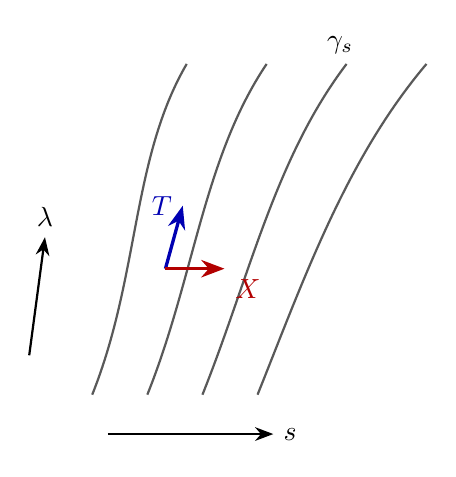
\begin{tikzpicture}[scale=1.0,>=Stealth]
  \foreach \s in {0,0.7,1.4,2.1}{
    \draw[thick,gray!70!black] (\s,0) .. controls (\s+0.6,1.5) and (\s+0.3*\s+0.5,3) .. (\s+0.45*\s+1.2,4.2);}
  \node[above] at (3.15,4.2) {$\gamma_s$};
  \draw[->,very thick,blue!70!black] (0.93,1.6) -- (1.15,2.4) node[left] {$T$};
  \draw[->,very thick,red!70!black] (0.93,1.6) -- (1.68,1.6) node[below right] {$X$};
  \draw[->,thick] (-0.8,0.5) -- (-0.6,2.0) node[above] {$\lambda$};
  \draw[->,thick] (0.2,-0.5) -- (2.3,-0.5) node[right] {$s$};
\end{tikzpicture}
\caption{A family of geodesics $\gamma_s$. The parameter $s$ labels the geodesic, $\lambda$ is the affine parameter along each geodesic. $T=\pd x/\pd\lambda$ is the tangent vector, $X=\pd x/\pd s$ the deviation vector connecting neighbouring geodesics.}
\label{fig:deviation}
\end{figure}

\begin{theorem}{Geodesic deviation equation}{deviation}
\begin{equation}
  A^\mu=\frac{D^2X^\mu}{\dd\lambda^2}=\Riem{\mu}{\nu}{\rho}{\sigma}\,T^\nu T^\rho X^\sigma .
\end{equation}
The relative acceleration between two neighbouring geodesics is proportional to the curvature.
\end{theorem}
\begin{proof}
(i) Since $x^\mu(s,\lambda)$ are coordinate functions, partial derivatives commute, $\pd_s T^\mu=\pd_\lambda X^\mu$. Using the symmetry of $\Gamma$,
$T^\rho D_\rho X^\mu=\pd_\lambda X^\mu+\Ga{\mu}{\rho}{\sigma}T^\rho X^\sigma=\pd_sT^\mu+\Ga{\mu}{\sigma}{\rho}X^\sigma T^\rho=X^\rho D_\rho T^\mu$.
(ii) Then $A^\mu=T^\rho D_\rho(X^\sigma D_\sigma T^\mu)=(T^\rho D_\rho X^\sigma)(D_\sigma T^\mu)+T^\rho X^\sigma D_\rho D_\sigma T^\mu$.
(iii) Write $D_\rho D_\sigma T^\mu=D_\sigma D_\rho T^\mu+\Riem{\mu}{\nu}{\rho}{\sigma}T^\nu$ by \eqref{eq:commutator}. Then
$T^\rho X^\sigma D_\sigma D_\rho T^\mu=X^\sigma D_\sigma(T^\rho D_\rho T^\mu)-(X^\sigma D_\sigma T^\rho)D_\rho T^\mu$. The first term vanishes because $T^\rho D_\rho T^\mu=0$ (geodesic equation). The second, using (i), is $-(T^\sigma D_\sigma X^\rho)D_\rho T^\mu$, which cancels the first term of (ii) (after relabelling). What remains is $A^\mu=\Riem{\mu}{\nu}{\rho}{\sigma}T^\rho X^\sigma T^\nu$.
\end{proof}

\paragraph{Newtonian analogue.} In the weak-field limit (\cref{ch:efe}) $g_{00}=1+2\Phi(\vec x)/c^2$, where $\Phi$ is the Newtonian potential. Two neighbouring particles separated by $\xi^i$ have relative acceleration $\ddot\xi^i=-\frac{\pd^2\Phi}{\pd x^i\pd x^j}\xi^j$: the relative acceleration involves second derivatives of the potential, the \textbf{tidal tensor} $\Delta_{ij}=\pd_i\pd_j\Phi$. In GR its role is played by $R^i{}_{0j0}$ (for slowly moving particles $T^\mu\simeq(c,\vec 0)$). In empty space the Newtonian field equation is $\nabla^2\Phi=0\Leftrightarrow\sum_i\Delta_{ii}=0$: the trace of the tidal tensor vanishes. The relativistic counterpart is $\Riem{\mu}{\alpha}{\mu}{\beta}\dot x^\alpha\dot x^\beta=R_{\alpha\beta}\dot x^\alpha\dot x^\beta=0$, which suggests that the vacuum field equations are $R_{\mu\nu}=0$. This is an important hint towards the Einstein field equations.

% =====================================================================
\chapter{The energy--momentum tensor}\label{ch:emt}
% =====================================================================

\paragraph{Motivation.} In Newtonian gravity, empty space is described by Laplace's equation $\nabla^2\Phi=0$; introducing matter, we get Poisson's equation
\[
  \nabla^2\Phi=(\text{const})\times\rho(\vec r)=4\pi\GN\rho(\vec r),
\]
where $\rho(\vec r)$ is the mass density at each point $\vec r$. Here we are trying to obtain the analogous equation in GR, but written with \emph{tensors}. We therefore need a tensorial object describing the matter (energy) content of space-time: the energy--momentum tensor. We first need a few reminders.

\section{Reminders: volume element and Gauss' theorem}

\paragraph{(i) The volume element.} $\dd^4x=\dd x^0\dd x^1\dd x^2\dd x^3$ is \emph{not} invariant under general coordinate transformations, which is a problem if we want to integrate densities. Under $x\to x'$,
\begin{equation}
  \dd^4x'=\left|\det\left(\frac{\pd x'^\mu}{\pd x^\nu}\right)\right|\dd^4x\equiv|J|\,\dd^4x ,
\end{equation}
with $J$ the Jacobian determinant of the transformation. On the other hand, from $g'_{\mu\nu}=\frac{\pd x^\alpha}{\pd x'^\mu}\frac{\pd x^\beta}{\pd x'^\nu}g_{\alpha\beta}$ (i.e.\ $g'=M^TgM$ with $\det M=J^{-1}$) and the multiplicativity of determinants,
\begin{equation}
  \det(g'_{\mu\nu})=J^{-1}J^{-1}\det(g_{\mu\nu})=J^{-2}\det(g_{\mu\nu}).
\end{equation}
Therefore $\sqrt{|\det g'|}=|J|^{-1}\sqrt{|\det g|}$ and the combination
\begin{equation}
  \boxed{\dd V=\sqrt{|\det(g_{\mu\nu})|}\,\dd^4x}\qquad\Longrightarrow\qquad\dd V'=\dd V
\end{equation}
is invariant: it is the \textbf{invariant volume element}. (In Minkowski space in inertial coordinates $|\det\eta|=1$; in spherical coordinates of flat 3-space, $\sqrt{\det g}=r^2\sin\theta$ and we recover $\dd V=r^2\sin\theta\,\dd r\,\dd\theta\,\dd\phi$.)

\paragraph{(ii) Gauss' theorem.} For a vector field $A^\mu$ and a 4-volume $\mathcal V$ with boundary $\pd\mathcal V$,
\begin{equation}
  \int_{\mathcal V}\dd^4x\sqrt{g}\,D_\mu A^\mu=\oint_{\pd\mathcal V}\dd^3x\sqrt{g_3}\,N_\mu A^\mu ,
\end{equation}
where $g\equiv|\det(g_{\mu\nu})|$, $g_3$ is the determinant of the induced metric on the 3-dimensional boundary and $N_\mu$ is the (unit) covector orthogonal to the boundary. (It is the 4D version of $\int_V\nabla\cdot\vec F\,\dd V=\oint_{\pd V}\vec F\cdot\dd\vec S$.) It relies on the useful identity $\sqrt g\,D_\mu A^\mu=\pd_\mu(\sqrt g A^\mu)$, which follows from $\Ga{\mu}{\mu}{\lambda}=\pd_\lambda\ln\sqrt g$.

\section{Densities in Minkowski space-time}

In 3D space, a density $\rho$ gives the number of particles $\dd N$ in a volume element $\dd V^3$:
\begin{equation}
  \dd N=\rho\,\dd V^3,\qquad N=\int\rho\,\dd V^3 .
  \label{eq:density3d}
\end{equation}
From a 4D perspective, however, a 3D volume acquires an \textbf{orientation}: we can move it along a vector with components $\dd x^\mu$, and the 4D volume swept is a scalar (it has no orientation):
\begin{equation}
  \dd V^4=\dd x^\mu\,\dd V_\mu ,
\end{equation}
where $\dd V_\mu$ is a 3D \emph{covector} volume element (``normal'' to the 3-volume, \cref{fig:dV}). For instance, for a 3-volume lying in the slice $t=0$, $\dd V_\mu=(\dd V^3,0,0,0)$, and moving it by $\dd x^\mu=(\dd t,\vec 0)$ sweeps $\dd V^4=\dd t\,\dd V^3$. The analogue of \eqref{eq:density3d} must then be
\begin{equation}
  \boxed{\dd N=\rho^\mu\,\dd V_\mu}:
\end{equation}
\textbf{densities become vectors}. Here $\dd N$ is the number of particles in the volume, $\rho^\mu$ the density 4-vector and $\dd V_\mu$ the 3D volume element in 4D space-time. For the slice $t=0$, $\dd N=\rho^0\dd V^3$: the time component of the density vector is the usual density.

\begin{figure}[ht]
\centering
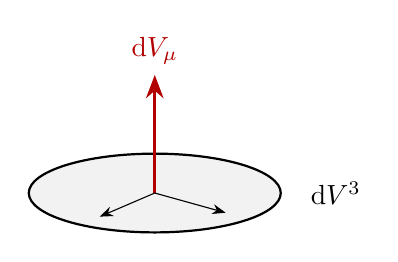
\begin{tikzpicture}[scale=1.0,>=Stealth]
  \draw[thick,fill=gray!10] (0,0) ellipse (1.6 and 0.5);
  \draw[->,very thick,red!70!black] (0,0) -- (0,1.5) node[above] {$\dd V_\mu$};
  \draw[->,thin] (0,0) -- (0.9,-0.25);
  \draw[->,thin] (0,0) -- (-0.7,-0.3);
  \node at (2.3,0) {$\dd V^3$};
\end{tikzpicture}
\caption{A 3-dimensional volume element in space-time is oriented: it is described by a covector $\dd V_\mu$ ``normal'' to it.}
\label{fig:dV}
\end{figure}

\subsection{Particle number density}

\textbf{Question 1:} \emph{how many world-lines cross a given 3-volume $V$?} (\cref{fig:numberdensity}, left). The answer is
\begin{equation}
  \dd N=n^\mu\dd V_\mu,\qquad N=\int_V n^\mu\dd V_\mu,
\end{equation}
where $n^\mu$ is the \textbf{number density vector}, and $N$ is a physical particle number.

\begin{figure}[ht]
\centering
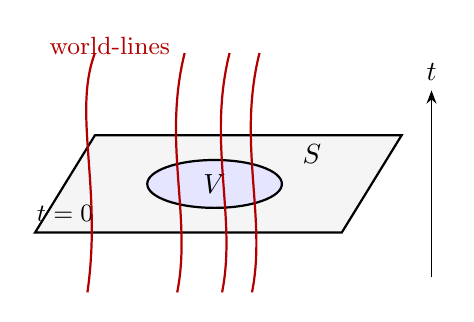
\begin{tikzpicture}[scale=0.95,>=Stealth]
  % slice t=0
  \draw[thick,fill=gray!8] (-2.3,-0.6) -- (1.8,-0.6) -- (2.6,0.7) -- (-1.5,0.7) -- cycle;
  \node at (-1.9,-0.35) {\small $t=0$};
  \draw[thick,fill=blue!10] (0.1,0.05) ellipse (0.9 and 0.32);
  \node at (0.1,0.05) {$V$};
  \node at (1.4,0.45) {$S$};
  \foreach \x in {-0.4,0.2,0.6}{\draw[red!70!black,thick] (\x,-1.4) .. controls (\x+0.2,-0.4) and (\x-0.2,0.6) .. (\x+0.1,1.8);}
  \draw[red!70!black,thick] (-1.6,-1.4) .. controls (-1.4,0) and (-1.8,1) .. (-1.5,1.8);
  \node[red!70!black] at (-1.3,1.9) {\small world-lines};
  \draw[->] (3,-1.2) -- (3,1.3) node[above] {$t$};
\end{tikzpicture}
\hspace{1.2cm}
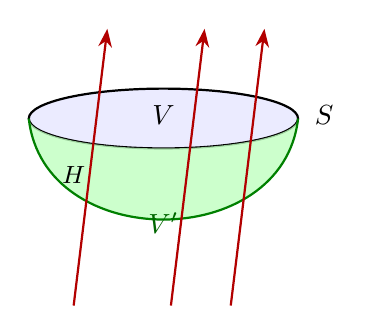
\begin{tikzpicture}[scale=0.95,>=Stealth]
  \draw[thick,fill=blue!8] (0,1.2) ellipse (1.8 and 0.4);
  \fill[green!25,opacity=0.8] (-1.8,1.2) .. controls (-1.6,-0.6) and (1.6,-0.6) .. (1.8,1.2) arc (0:-180:1.8 and 0.4);
  \draw[thick,green!50!black] (-1.8,1.2) .. controls (-1.6,-0.6) and (1.6,-0.6) .. (1.8,1.2);
  \node at (0,1.25) {$V$};
  \node[green!40!black] at (0,-0.2) {$V'$};
  \node at (2.15,1.25) {$S$};
  \node at (-1.2,0.45) {\small $H$};
  \foreach \x/\y in {-1.0/0.6,0.3/-0.3,1.1/0.4}{\draw[red!70!black,thick,->] (\x-0.2,-1.3) -- (\x+0.25,2.4);}
\end{tikzpicture}
\caption{Left: world-lines crossing a 3-volume $V$ (with boundary $S$) in the slice $t=0$ (one spatial dimension suppressed). Right: two 3-volumes $V$ and $V'$ with the same boundary $S$ enclose a 4-dimensional hypervolume $H$; every world-line crossing $V$ also crosses $V'$.}
\label{fig:numberdensity}
\end{figure}

\textbf{Question 2:} \emph{what does particle number conservation look like?} The number of particles is a physical quantity and does not change. Consider another 3-volume $V'$ with the same boundary $S$ as $V$ (\cref{fig:numberdensity}, right). If particles are neither created nor destroyed, every world-line crossing $V$ also crosses $V'$ exactly once. $V$ and $V'$ together form the boundary of a 4-dimensional hypervolume $H$, and the difference of the integrals over $V$ and $V'$ is, by Gauss' theorem,
\begin{equation}
  \int_H\pd_\mu n^\mu\,\dd^4H=0 .
\end{equation}
This must be true for all $H$, hence
\begin{equation}
  \boxed{\pd_\mu n^\mu=0}\qquad\Longleftrightarrow\qquad\pd_t n^0=-\nabla\cdot\vec n :
\end{equation}
the \textbf{continuity equation} (the density change rate is minus the divergence of the flow). One can also write $n^\mu(x)=n(x)V^\mu(x)$, where $n(x)$ is the \emph{scalar} density (number per unit volume in the rest frame) and $V^\mu$ the 4-velocity field. In the same way we can think about densities of other quantities.

\section{The stress--energy--momentum tensor}

Consider a particle moving with 4-velocity (we set $c=1$ in this section)
\begin{equation}
  V^\mu=\frac{\dd x^\mu}{\dd\tau}=\frac{\dd x^\mu}{\dd t}\frac{\dd t}{\dd\tau}=\begin{cases}(1,0,0,0)&\text{in its own rest frame},\\ \gamma(1,v^x,v^y,v^z)&\text{in any other frame.}\end{cases}
\end{equation}
It carries the 4-momentum $p^\mu=m\gamma(1,v^x,v^y,v^z)=mV^\mu$.

\textbf{Question:} what is the total 4-momentum carried by a set of particles contained in (or flowing through) a 3-volume $V$? Momentum is itself a vector, so its density must be a vector-valued density, i.e.\ a $(2,0)$ tensor: we can write
\begin{equation}
  P^\mu=\int_V T^{\mu\nu}\,\dd V_\nu ,
\end{equation}
which defines the \textbf{stress--energy--momentum tensor} $T^{\mu\nu}$. In SR $P^\mu$ is conserved, so, by the same argument as for $n^\mu$,
\begin{equation}
  \int_H\pd_\mu T^{\mu\nu}\,\dd^4H=0\quad\forall H\qquad\Longrightarrow\qquad\boxed{\pd_\mu T^{\mu\nu}=0}\quad\text{(in SR)}.
\end{equation}

\paragraph{Definition for an ensemble of identical particles.} In practice we define
\begin{equation}
  T^{\mu\nu}\equiv n\,p^\mu V^\nu=\underbrace{n\,m}_{\rho(x)}V^\mu V^\nu ,
\end{equation}
the flow of $\mu$-momentum through a unit surface of constant $x^\nu$. The interpretation of its components is:
\begin{enumerate}[label=(\roman*),nosep]
  \item $T^{00}$: \textbf{energy density};
  \item $T^{0i}$: \textbf{energy flow} (flux) in the $i$-th direction;
  \item $T^{i0}$: density of the $i$-th component of \textbf{momentum};
  \item $T^{ij}$: flow of the $i$-th component of momentum in the $j$-th direction: the \textbf{stress tensor}.
\end{enumerate}
The tensor is symmetric, $T^{\mu\nu}=T^{\nu\mu}$ (energy flux $=$ momentum density, with $c=1$).

\paragraph{Physical meaning of $T^{ij}$: pressure.} Consider a ``small box'' and particles coming from the left with velocity $v^i$, hitting one of its faces, of area $\dd S_n$, with normal $\vec e_j$ (\cref{fig:box}). In a time $\dd t$, the particles which hit the face are those contained in a slab of thickness $v\,\dd t$, i.e.\ $n(\vec v\dd t)\cdot\dd\vec S_n$ of them, each one carrying momentum $p^i$. The momentum transferred to the face is
\begin{equation}
  \dd p^i=n\,(\vec v\dd t)\cdot\dd\vec S_n\,p^i\equiv K^i\dd t=F^i\dd t ,
\end{equation}
where $[K^i]=\mathrm{kg\,m\,s^{-2}}$ is a force. For $i=j$ (normal incidence) the force per unit area is a \textbf{pressure}:
\begin{equation}
  T^{ii}=n\,m\,(v^i)^2\quad\text{(pressure in the box)}.
\end{equation}
If $\dd p^i>0$, momentum is transferred to the surface, $F^i>0$, $P_{\rm in}>0$, $T^{ii}>0$.

\begin{figure}[ht]
\centering
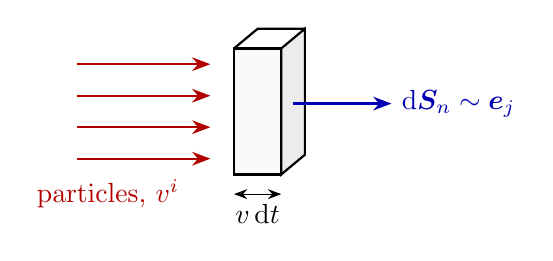
\begin{tikzpicture}[scale=1.0,>=Stealth]
  \foreach \y in {0.2,0.6,1.0,1.4}{\draw[->,thick,red!70!black] (-2.6,\y) -- (-0.9,\y);}
  \node[red!70!black] at (-2.2,-0.25) {particles, $v^i$};
  \draw[thick,fill=gray!15] (0,0) -- (0.3,0.25) -- (0.3,1.85) -- (0,1.6) -- cycle;
  \draw[thick,fill=gray!5] (-0.6,0) -- (0,0) -- (0,1.6) -- (-0.6,1.6) -- cycle;
  \draw[thick] (-0.6,1.6) -- (-0.3,1.85) -- (0.3,1.85);
  \draw[<->] (-0.6,-0.25) -- (0,-0.25) node[midway,below] {$v\,\dd t$};
  \draw[->,thick,blue!70!black] (0.15,0.9) -- (1.4,0.9) node[right] {$\dd\vec S_n\sim\vec e_j$};
\end{tikzpicture}
\caption{Particles with velocity $v^i$ hit a face of area $\dd S_n$ (normal $\vec e_j$). In a time $\dd t$ all particles in the slab of thickness $v\,\dd t$ hit the face and transfer their momentum: $T^{ij}$ is the flux of $i$-momentum through the surface orthogonal to $j$, i.e.\ a stress (pressure for $i=j$).}
\label{fig:box}
\end{figure}

\section{Conservation law in curved space-time}

Assume that all the particles have the same 4-velocity field and travel along geodesics (free particles). Then:
\begin{enumerate}
\item they have zero covariant acceleration:
\begin{equation}
  a^\mu=\frac{DV^\mu(x(\tau))}{\dd\tau}=\frac{\dd x^\nu}{\dd\tau}D_\nu V^\mu(x)=V^\nu D_\nu V^\mu=0 ;
\end{equation}
\item particles neither appear nor disappear (covariant continuity equation): $D_\mu\big(n(x)V^\mu(x)\big)=0$.
\end{enumerate}
Then, by the Leibniz rule,
\begin{equation}
  D_\mu T^{\mu\nu}=D_\mu\big(m\,n\,V^\mu V^\nu\big)=m V^\nu\underbrace{D_\mu\big(nV^\mu\big)}_{=0\ \text{(continuity)}}+m\,n\,\underbrace{V^\mu D_\mu V^\nu}_{=0\ \text{(geodesics)}}=0 .
\end{equation}

\begin{keyresult}[Covariant conservation of energy and momentum]
\begin{equation}
  D_\mu T^{\mu\nu}=0 .
\end{equation}
This is the generalisation to curved space-time of $\pd_\mu T^{\mu\nu}=0$ (``comma goes to semicolon''). Note that, unlike $\pd_\mu T^{\mu\nu}=0$ in SR, it does not imply the existence of a globally conserved total energy: energy can be exchanged with the gravitational field.
\end{keyresult}

\section{Special cases}

\paragraph{1) Immobile dust.} A set of particles at rest (pressureless matter): the world-lines are all parallel to the $t$ axis, $V^\mu=(1,0,0,0)$. This implies
\begin{equation}
  T^{00}=\rho_0,\qquad T^{\mu\nu}=0\ \text{otherwise},
\end{equation}
with $\rho_0$ the rest mass density.

\paragraph{2) Constant-velocity (generic) dust.} For an observer moving along with the dust we come back to case 1: $T^{\mu\nu}=\rho_0V^\mu V^\nu$ with $V^\mu=(1,\vec 0)$. For any other observer, $V^\mu=\gamma(1,v^x,v^y,v^z)$ and
\begin{equation}
  T^{\mu\nu}=\rho_0\gamma^2\begin{pmatrix}1&v^x&v^y&v^z\\ v^x&(v^x)^2&v^xv^y&v^xv^z\\ v^y&v^yv^x&(v^y)^2&v^yv^z\\ v^z&v^zv^x&v^zv^y&(v^z)^2\end{pmatrix}.
\end{equation}
Now the mass current ($T^{0i}$) is non-zero and the stress ($T^{ij}$) is non-zero. Note the factor $\gamma^2$: one $\gamma$ from the Lorentz contraction of the volume (the number density increases, $n=\gamma n_0$) and one from the energy of each particle ($E=\gamma m$).

\paragraph{3) Static mono-energetic gas.} A set of particles with the same speed $v$ (velocity measure) but random directions. Averaging $T^{\mu\nu}=\rho_0\gamma^2(1,v^i)\otimes(1,v^j)$ over directions: $\langle v^i\rangle=0$, $\langle v^iv^j\rangle=0$ for $i\neq j$, and by isotropy $\langle(v^x)^2\rangle=\langle(v^y)^2\rangle=\langle(v^z)^2\rangle=v^2/3$. Hence
\begin{equation}
  T^{\mu\nu}=\rho_0\gamma^2\begin{pmatrix}1&0&0&0\\0&v^2/3&0&0\\0&0&v^2/3&0\\0&0&0&v^2/3\end{pmatrix}:
\end{equation}
an \textbf{isotropic stress}, i.e.\ a pressure $p=\frac13\rho_0\gamma^2v^2$.

\paragraph{4) Static ideal (perfect) gas.} The particles follow a statistical distribution of velocities; in the rest frame of the gas
\begin{equation}
  T^{\mu\nu}=\begin{pmatrix}\rho&0&0&0\\0&p&0&0\\0&0&p&0\\0&0&0&p\end{pmatrix},
\end{equation}
where $\rho$ is the average energy (mass) density and $p$ the average pressure, related through an equation of state (e.g.\ the ideal-gas law). Since in the rest frame $V^\mu=(1,0,0,0)$ and $g^{\mu\nu}=\eta^{\mu\nu}=\mathrm{diag}(1,-1,-1,-1)$, this can be written in the covariant form
\begin{equation}
  \boxed{T^{\mu\nu}=(\rho+p)V^\mu V^\nu-p\,g^{\mu\nu}}
\end{equation}
(check: $T^{00}=(\rho+p)-p=\rho$, $T^{ii}=0-p(-1)=p$). Being a tensor equation, it is valid in any frame, also for an observer moving with respect to the gas, and locally in curved space-time. This is the \textbf{perfect fluid} energy--momentum tensor, used e.g.\ for stars (Problem Sheet 4) and in cosmology.

\paragraph{5) Radiation.} For a gas of photons (or ultra-relativistic particles) $v\to1$ in case 3 and the pressure is $p_R=\rho/3$. Then
\begin{equation}
  T^{\mu\nu}=\frac43\rho\,V^\mu V^\nu-\frac13\rho\,g^{\mu\nu}=\mathrm{diag}\Big(\rho,\frac\rho3,\frac\rho3,\frac\rho3\Big)\quad\text{(rest frame)},
\end{equation}
which is traceless: $T^\mu{}_\mu=g_{\mu\nu}T^{\mu\nu}=\rho-3p=0$.

% =====================================================================
\chapter{Newtonian limit and the Einstein field equations}\label{ch:efe}
% =====================================================================

\section{Newtonian limit of the geodesic equations}

We would like the geodesic equations to reduce, in an appropriate limit, to Newton's equation of motion in a gravitational potential,
\begin{equation}
  \frac{\dd^2\vec x}{\dd t^2}=-\nabla\Phi ,\qquad\text{e.g.}\quad\Phi=-\frac{\GN M}{r},
\end{equation}
but now in a \emph{curved} space-time. We set $c=1$ and restore it at the end.

\begin{definition}{Newtonian limit}{newt-limit}
The Newtonian limit is defined by three requirements:
\begin{enumerate}
\item \textbf{Weak fields:} in some appropriate coordinates the metric is a small perturbation of flat space,
\begin{equation}
  g_{\mu\nu}=\eta_{\mu\nu}+h_{\mu\nu},\qquad|h_{\mu\nu}|\ll1,
\end{equation}
and we keep only terms linear in $h_{\mu\nu}$ and its derivatives (this is a statement about the field \emph{and} the coordinates).
\item \textbf{Small velocities:} $\left|\frac{\dd x^i}{\dd t}\right|\ll1\ \Longleftrightarrow\ \left|\frac{\dd x^i}{\dd\tau}\right|\ll\frac{\dd t}{\dd\tau}$ (particles move slowly).
\item \textbf{Stationary fields:} $\pd_0g_{\mu\nu}=0\ \Longleftrightarrow\ \pd_0h_{\mu\nu}=0$ (fields unchanging with time).
\end{enumerate}
\end{definition}

\begin{warningbox}[The inverse metric]
Concerning the inverse metric, $g^{\mu\nu}\simeq\eta^{\mu\nu}\,\boldsymbol{-}\,h^{\mu\nu}$ with $h^{\mu\nu}\equiv\eta^{\mu\alpha}\eta^{\nu\beta}h_{\alpha\beta}$ (note the minus sign!). This follows from the matrix identity $(I+A)^{-1}=I-A+\order{A^2}$, or directly: writing $g^{\mu\nu}=\eta^{\mu\nu}+H^{\mu\nu}$,
\[
  g_{\mu\nu}g^{\nu\rho}=(\eta_{\mu\nu}+h_{\mu\nu})(\eta^{\nu\rho}+H^{\nu\rho})=\delta_\mu{}^\rho+\eta_{\mu\nu}H^{\nu\rho}+h_{\mu\nu}\eta^{\nu\rho}+\order{hH}\overset{!}{=}\delta_\mu{}^\rho ,
\]
so $\eta_{\mu\nu}H^{\nu\rho}=-h_\mu{}^\rho$, i.e.\ $H^{\mu\rho}=-h^{\mu\rho}$.
\end{warningbox}

\paragraph{The geodesic equation.}
\[
  \frac{\dd^2x^\mu}{\dd\tau^2}+\Ga{\mu}{\nu}{\lambda}\frac{\dd x^\nu}{\dd\tau}\frac{\dd x^\lambda}{\dd\tau}=0,\qquad
  \Ga{\mu}{\nu}{\lambda}=\frac12 g^{\mu\alpha}\left(\pd_\nu g_{\lambda\alpha}+\pd_\lambda g_{\nu\alpha}-\pd_\alpha g_{\nu\lambda}\right).
\]
\begin{itemize}
\item \emph{Weak fields:} since $\pd\eta=0$, the bracket is already of order $h$, so we can replace $g^{\mu\alpha}\to\eta^{\mu\alpha}$:
\[
  \Ga{\mu}{\nu}{\lambda}\simeq\frac12\eta^{\mu\alpha}\left(\pd_\nu h_{\lambda\alpha}+\pd_\lambda h_{\nu\alpha}-\pd_\alpha h_{\nu\lambda}\right).
\]
\item \emph{Small velocities:} $\frac{\dd x^i}{\dd\tau}\ll\frac{\dd t}{\dd\tau}$, so in the sum over $\nu,\lambda$ the term with $\nu=\lambda=0$ dominates (the terms $\Ga{\mu}{i}{j}\frac{\dd x^i}{\dd\tau}\frac{\dd x^j}{\dd\tau}$ and $\Ga{\mu}{0}{i}\frac{\dd t}{\dd\tau}\frac{\dd x^i}{\dd\tau}$ are suppressed by powers of $v$):
\[
  \frac{\dd^2x^\mu}{\dd\tau^2}+\Ga{\mu}{0}{0}\frac{\dd t}{\dd\tau}\frac{\dd t}{\dd\tau}=0,
\]
so we only need $\Ga{\mu}{0}{0}=\frac12 g^{\mu\alpha}\big(\pd_0g_{0\alpha}+\pd_0g_{0\alpha}-\pd_\alpha g_{00}\big)$.
\item \emph{Stationary fields:} $\pd_0g_{0\alpha}=0$, so
\[
  \Ga{\mu}{0}{0}=-\frac12\eta^{\mu\alpha}\pd_\alpha h_{00}=-\frac12\eta^{\mu i}\pd_ih_{00}
\]
(the $\alpha=0$ term vanishes as $\pd_0h_{00}=0$). With the signature $(+,-,-,-)$, $\eta^{ij}=-\delta^{ij}$, and therefore
\begin{equation}
  \Ga{0}{0}{0}=0,\qquad\Ga{i}{0}{0}=\frac12\pd_ih_{00}.
\end{equation}
\end{itemize}
All in all,
\begin{equation}
  \frac{\dd^2x^\mu}{\dd\tau^2}+\Ga{\mu}{0}{0}\frac{\dd t}{\dd\tau}\frac{\dd t}{\dd\tau}=0\quad\Longrightarrow\quad
  \begin{cases}\dfrac{\dd^2t}{\dd\tau^2}=0 &\Rightarrow\ t(\tau)=a\tau+b,\qquad(1)\\[2ex]
  \dfrac{\dd^2x^i}{\dd\tau^2}=-\dfrac12\pd_ih_{00}\left(\dfrac{\dd t}{\dd\tau}\right)^2.&\qquad(2)\end{cases}
\end{equation}
Equation (1) reflects the fact that there is no difference (up to an affine rescaling) between $t$ and $\tau$ in Newtonian mechanics. For the left-hand side of (2), by the chain rule,
\[
  \frac{\dd^2x^i}{\dd\tau^2}=\frac{\dd}{\dd\tau}\left(\frac{\dd t}{\dd\tau}\frac{\dd x^i}{\dd t}\right)=\frac{\dd^2t}{\dd\tau^2}\frac{\dd x^i}{\dd t}+\left(\frac{\dd t}{\dd\tau}\right)^2\frac{\dd^2x^i}{\dd t^2}
  =\left(\frac{\dd t}{\dd\tau}\right)^2\frac{\dd^2x^i}{\dd t^2},
\]
since $\dd^2t/\dd\tau^2=0$ from (1). Going back to (2), the factor $(\dd t/\dd\tau)^2$ cancels:
\begin{equation}
  \frac{\dd^2x^i}{\dd t^2}=-\frac12\pd_ih_{00}.
\end{equation}
Comparing with Newton, $\frac{\dd^2x^i}{\dd t^2}=-\pd_i\Phi$, we identify $h_{00}=2\Phi$ (up to an irrelevant constant, fixed by requiring $h\to0$ far from sources), i.e.
\begin{keyresult}[Newtonian limit]
\begin{equation}
  g_{00}=1+2\Phi\qquad\Big(g_{00}=1+\frac{2\Phi}{c^2}\ \text{restoring}\ c\Big).
\end{equation}
Newtonian mechanics is captured by GR assuming a space-time with
\begin{equation}
  \dd s^2=\big(1+2\Phi(\vec x)\big)\dd t^2-\dd\vec x^{\,2}.
\end{equation}
\end{keyresult}
The curvature of space-time (more precisely, of its time--time component) is sufficient to describe gravity in the Newtonian limit.

\begin{remarkbox}[Remarks]
\begin{enumerate}[label=(\roman*),nosep]
\item For a radial gravitational field, $\dd s^2=(1+2\Phi(r))\dd t^2-\dd r^2-r^2\dd\Omega_2^2$, with $\dd\Omega_2^2=\dd\theta^2+\sin^2\theta\,\dd\phi^2$ the line element on the unit 2-sphere.
\item If $c\neq1$: $g_{00}=1+2\Phi/c^2$. Since $|\Phi|/c^2\sim10^{-9}$ at the surface of the Earth and $10^{-6}$ at the surface of the Sun, the weak-field approximation is excellent in the solar system.
\item With the signature $(-,+,+,+)$ one has instead $g_{00}=-(1+2\Phi)$.
\item In Minkowski space, spatial indices are raised and lowered with $\eta_{ij}=-\delta_{ij}$, hence $\pd^i=-\pd_i$; with this, $\Ga{i}{0}{0}=-\frac12\pd^ih_{00}$.
\end{enumerate}
\end{remarkbox}

\section{The Einstein field equations}

\subsection{Looking for the field equations}
In Newtonian mechanics the gravitational potential is determined by the mass density through Poisson's equation
\begin{equation}
  \nabla^2\Phi=4\pi\GN\rho .\tag{1}
\end{equation}
From the previous section $g_{00}=1+2\Phi$ (2). Identifying, on top, $T_{00}=\rho$ (the energy density of non-relativistic matter is dominated by its rest mass) we find
\begin{equation}
  \nabla^2g_{00}=8\pi\GN T_{00}.
\end{equation}
This suggests to look for a tensor equation of the form
\begin{equation}
  E_{\mu\nu}=8\pi\GN T_{\mu\nu}.
\end{equation}
What is $E_{\mu\nu}$? Sensible requirements are:
\begin{enumerate}
\item $E_{\mu\nu}$ is a \textbf{tensor};
\item it has the dimension of second derivatives of the metric, i.e.\ it is linear in second derivatives or quadratic in first derivatives of $g_{\mu\nu}$ (like $\nabla^2\Phi$);
\item it is \textbf{symmetric} (as $T_{\mu\nu}$);
\item it is \textbf{covariantly conserved}, $D^\mu E_{\mu\nu}=0$ (as $T_{\mu\nu}$, see \cref{ch:emt});
\item in the Newtonian limit, $E_{00}=\nabla^2g_{00}$.
\end{enumerate}
We construct $E_{\mu\nu}$ with the tensors we have previously defined.
\begin{itemize}
\item Requirements 1) and 2) leave (essentially) the combination
\[
  E_{\mu\nu}=aR_{\mu\nu}+b\,g_{\mu\nu}R ,
\]
since the Riemann tensor is the only tensor built with second derivatives of the metric, and its only rank-2 contractions are $R_{\mu\nu}$ and $g_{\mu\nu}R$. Requirement 3) is then automatically satisfied.
\item For requirement 4), we rewrite it in terms of the Einstein tensor: $E_{\mu\nu}=aG_{\mu\nu}+c\,g_{\mu\nu}R$ (with $c=b+a/2$). We saw that $D^\mu G_{\mu\nu}=0$ and $D^\mu g_{\mu\nu}=0$, hence
\[
  D^\mu E_{\mu\nu}=c\,g_{\mu\nu}D^\mu R=c\,D_\nu R\overset{!}{=}0\quad\Longrightarrow\quad\text{either }D_\nu R=0\ \text{or}\ c=0 .
\]
\item Observe that, taking the trace (with $g^{\mu\nu}g_{\mu\nu}=\delta^\mu{}_\mu=4$),
\[
  g^{\mu\nu}E_{\mu\nu}=a\,g^{\mu\nu}G_{\mu\nu}+c\,g^{\mu\nu}g_{\mu\nu}R=a(R-2R)+4cR=(4c-a)R ,
\]
which must also be equal to $8\pi\GN T^\mu{}_\mu$. If $c\neq0$ we would need $D_\nu R=0$, i.e.\ $R$ constant, hence $T^\mu{}_\mu$ constant all over space-time: we could not describe \emph{any} distribution of matter we like. This is physically inconsistent, so we choose $c=0$:
\begin{equation}
  E_{\mu\nu}=a\,G_{\mu\nu},
\end{equation}
and now ``$a$'' is left to be calculated.
\end{itemize}

\paragraph{Fixing $a$ with the Newtonian limit.} Take requirement 5): weak fields ($g=\eta+h$, linear in $h$), stationary ($\pd_0g_{\mu\nu}=0$), non-relativistic source: $T_{00}=\rho$ and $T_{\mu\nu}\simeq0$ otherwise (pressures and momentum densities are suppressed by powers of $v^2$). Then we only need $E_{00}=aG_{00}$.
\begin{itemize}
\item $G_{00}=R_{00}-\frac12g_{00}R\simeq R_{00}-\frac12R$, at linear order in $h$ (since $R$ is already of order $h$, $g_{00}R\simeq\eta_{00}R=R$).
\item $T_{ij}=0\Rightarrow G_{ij}=0\Rightarrow R_{ij}=\frac12 g_{ij}R\simeq\frac12\eta_{ij}R=-\frac12\delta_{ij}R$.
\item Combining the last two: $R=g^{\mu\nu}R_{\mu\nu}\simeq\eta^{\mu\nu}R_{\mu\nu}=R_{00}-\delta^{ij}R_{ij}=R_{00}+\frac32R$, hence $\boxed{R=-2R_{00}}$.
\item Therefore $G_{00}=R_{00}-\frac12R=R_{00}+R_{00}=2R_{00}$, with $R_{00}=\Riem{\mu}{0}{\mu}{0}$.
\end{itemize}

\begin{exercise}{Weak static fields}{R00}
Show that, for time-independent fields in the weak-field limit, $R_{00}=\frac12\nabla^2g_{00}$.

\textit{Solution.} From \eqref{eq:riemann}, $R_{00}=\Riem{\mu}{0}{\mu}{0}=\pd_\mu\Ga{\mu}{0}{0}-\pd_0\Ga{\mu}{\mu}{0}+\Ga{\mu}{\mu}{\lambda}\Ga{\lambda}{0}{0}-\Ga{\mu}{0}{\lambda}\Ga{\lambda}{\mu}{0}$. The $\Gamma\Gamma$ terms are $\order{h^2}$ and are dropped; $\pd_0(\dots)=0$ for static fields. Hence, using $\Ga{0}{0}{0}=0$ and $\Ga{i}{0}{0}=\frac12\pd_ih_{00}$ computed above,
\[
  R_{00}\simeq\pd_i\Ga{i}{0}{0}=\frac12\pd_i\pd_ih_{00}=\frac12\nabla^2h_{00}=\frac12\nabla^2g_{00}. \qquad\blacksquare
\]
\end{exercise}

Using this result, $G_{00}=2R_{00}=\nabla^2g_{00}$. For requirement 5) to hold, $E_{00}=aG_{00}=\nabla^2g_{00}$, hence $a=1$. Therefore we have:

\begin{keyresult}[The Einstein field equations]
\begin{equation}
  \boxed{R_{\mu\nu}-\frac12g_{\mu\nu}R=8\pi\GN T_{\mu\nu}}\qquad\Big(=\frac{8\pi\GN}{c^4}T_{\mu\nu}\ \text{restoring}\ c\Big).
  \label{eq:efe}
\end{equation}
They tell us how the curvature of space-time reacts to the presence of energy and momentum.
\end{keyresult}

\paragraph{Check of the Newtonian limit.} $G_{00}=\nabla^2g_{00}=2\nabla^2\Phi$ and $8\pi\GN T_{00}=8\pi\GN\rho$: the $00$ component of \eqref{eq:efe} is exactly Poisson's equation $\nabla^2\Phi=4\pi\GN\rho$.

\paragraph{Trace-reversed form.} Taking the trace of \eqref{eq:efe}: $R-2R=-R=8\pi\GN T$, with $T\equiv T^\mu{}_\mu$. Substituting $R=-8\pi\GN T$ back,
\begin{equation}
  R_{\mu\nu}=8\pi\GN\Big(T_{\mu\nu}-\frac12Tg_{\mu\nu}\Big)
\end{equation}
(see Problem Sheet 4). In vacuum, $T_{\mu\nu}=0\Leftrightarrow R_{\mu\nu}=0$, in agreement with the hint from geodesic deviation (\cref{sec:geodesic-deviation}).

\subsection{Remarks}
\begin{enumerate}[label=(\roman*)]
\item For a given distribution of matter, energy, stress, etc., the EFE give us the \textbf{metric} (they are partial differential equations for $g_{\mu\nu}$).
\item In principle the EFE are a set of $10$ coupled, non-linear partial differential equations (one for each independent component of the symmetric tensors).
\item However, due to the (contracted) Bianchi identities $D^\mu G_{\mu\nu}=0$ (4 equations), there are only $6$ independent equations. This matches the fact that the metric has $10$ components, of which $4$ can be changed arbitrarily by a coordinate transformation $x\to x'(x)$ (4 functions): the metric is determined up to coordinate choices.
\item The ``algorithm'' of GR: given a distribution of matter,
\[
  \text{energy--momentum tensor}\ \xrightarrow{\ \text{EFE}\ }\ \text{metric}\ \longrightarrow\ \text{geodesics (equations of motion)}.
\]
(The Christoffel symbols are computed from the metric, and they determine how objects move.) In general, of course, matter and geometry must be solved for together, since matter moves according to the geometry it creates ($D_\mu T^{\mu\nu}=0$ is a consequence of the EFE).
\item Sadly, even in vacuum no closed-form \emph{general} solution is known. We must make simplifying assumptions (symmetries).
\item If $c\neq1$: $8\pi\GN\to8\pi\GN/c^4$.
\item In higher dimensions we still get equations of the form $G_{\mu\nu}=kT_{\mu\nu}$, but with different coefficients (and more complicated physics).
\item Including the \textbf{cosmological constant} term (allowed by requirement 4, since $D^\mu g_{\mu\nu}=0$; it only violates requirement 2):
\begin{equation}
  R_{\mu\nu}-\frac12g_{\mu\nu}R-\Lambda g_{\mu\nu}=8\pi\GN T_{\mu\nu}.
\end{equation}
\begin{itemize}[nosep]
\item Moving it to the right-hand side, $\Lambda g_{\mu\nu}=8\pi\GN T^{(\Lambda)}_{\mu\nu}$ with $T^{(\Lambda)}_{\mu\nu}=\rho_\Lambda g_{\mu\nu}$, $\rho_\Lambda=\Lambda/8\pi\GN$. Comparing with the perfect fluid $T_{\mu\nu}=(\rho+p)u_\mu u_\nu-pg_{\mu\nu}$, this is a fluid with $p_\Lambda=-\rho_\Lambda$: for $\Lambda>0$ the cosmological constant can be interpreted as a \textbf{negative pressure}.
\item Negative pressure makes the ``box'' (the Universe) expand; positive pressure makes it contract (attract).
\item It is treated as a numerical constant, an effective parametrisation of something we do not know: \textbf{dark energy}, responsible for the observed accelerated expansion of the Universe.
\end{itemize}
(With the opposite signature or curvature sign conventions, the sign in front of $\Lambda$ changes; what is physical is that $\Lambda>0$ corresponds to accelerated expansion.)
\end{enumerate}


\part{Applications}
% =====================================================================
\chapter{The Schwarzschild metric}\label{ch:schwarzschild}
% =====================================================================

The Schwarzschild solution describes the gravitational field outside a spherically symmetric body, such as the Earth or the Sun (to a very good approximation). It is the simplest and most important exact solution of the EFE.

\section{Assumptions and the form of the metric}

We are looking for a solution of the EFE:
\begin{enumerate}[label=\arabic*),start=0,nosep]
\item in \textbf{vacuum}, $T_{\mu\nu}=0\Rightarrow G_{\mu\nu}=0$;
\item in $(1+3)$ dimensions, working with the $(+,-,-,-)$ metric;
\item \textbf{spherically symmetric};
\item \textbf{static}.
\end{enumerate}
We work in ``spherical coordinates'' $(t,r,\theta,\phi)$ (Schwarzschild coordinates).

\paragraph{The metric is diagonal.} From requirements 2) and 3), the metric must be invariant under the discrete transformations
\begin{align*}
  (t,r,\theta,\phi)&\to(-t,r,\theta,\phi)\quad\text{(static: time reversal)},\\
  (t,r,\theta,\phi)&\to(t,r,-\theta,\phi)\quad\text{(spherical symmetry: reflection)},\\
  (t,r,\theta,\phi)&\to(t,r,\theta,-\phi)\quad\text{(spherical symmetry: reflection)},
\end{align*}
i.e.\ $g'_{\mu\nu}(x)=g_{\mu\nu}(x)$. But $g_{\mu\nu}$ is a $(0,2)$ tensor, $g'_{\mu\nu}=\frac{\pd x^\alpha}{\pd x'^\mu}\frac{\pd x^\beta}{\pd x'^\nu}g_{\alpha\beta}$. Consider $t\to-t$: the only non-trivial Jacobian element is $\pd t/\pd t'=-1$, so
\[
  g'_{00}=\frac{\pd x^\alpha}{\pd(-t)}\frac{\pd x^\beta}{\pd(-t)}g_{\alpha\beta}=g_{00},\qquad
  g'_{0r}=\frac{\pd x^\alpha}{\pd(-t)}\frac{\pd x^\beta}{\pd r}g_{\alpha\beta}=-g_{0r},\qquad g'_{0\nu}=-g_{0\nu}\ \ (\nu\neq0).
\]
The static condition requires $g'_{0\nu}=g_{0\nu}$, hence $g_{0\nu}=0$ for all $\nu\neq0$. Working similarly with the other two reflections, $g_{2\nu}=0$ for $\nu\neq2$ and $g_{3\nu}=0$ for $\nu\neq3$. Gathering things: $g_{\mu\nu}=0$ for all $\mu\neq\nu$: \textbf{the metric is diagonal} (in this coordinate system).

\paragraph{Spherical symmetry.}
\begin{enumerate}[label=(\roman*),nosep]
\item On each radial line ($\theta,\phi=$ const), $g_{rr}$ and $g_{tt}$ can only depend on $r$ (not on $t$, due to the static condition).
\item On the hypersurfaces $t,r=\text{const}$ the metric should take the form of that of a 2-sphere.
\end{enumerate}
Therefore
\[
  c^2\dd\tau^2=A(r)\dd t^2-B(r)\dd r^2-D(r)\,r^2\big(\dd\theta^2+\sin^2\theta\,\dd\phi^2\big).
\]
$D(r)$ can be eliminated by a coordinate transformation $r\to R(r)$ such that $R^2=D(r)r^2$ (this redefines $A$ and $B$); for simplicity we keep denoting the new radial coordinate by $r$:
\begin{equation}
  c^2\dd\tau^2=A(r)\dd t^2-B(r)\dd r^2-r^2\big(\dd\theta^2+\sin^2\theta\,\dd\phi^2\big).
  \label{eq:schw-ansatz}
\end{equation}
We now want to determine $A(r)$ and $B(r)$. Note that, because $\dd t$ and $\dd r$ are multiplied by functions, $t$ and $r$ are not, in general, proper time and proper distance.

\section{Solving the Einstein equations}

\paragraph{Vacuum equations.} Note that
\[
  G_{\mu\nu}=0\ \Rightarrow\ g^{\mu\nu}G_{\mu\nu}=g^{\mu\nu}\Big(R_{\mu\nu}-\frac12g_{\mu\nu}R\Big)=R-2R=-R=0\ \Rightarrow\ R=0 ,
\]
so $G_{\mu\nu}=0$ reduces to $\boxed{R_{\mu\nu}=0}$. Manifolds satisfying this are called \textbf{Ricci-flat}. The steps to solve the equations are:
\begin{enumerate}[nosep]
\item compute the $\Gamma$'s;
\item compute $\Riem{\mu}{\nu}{\rho}{\sigma}$ (actually not needed, see below);
\item compute $R_{\mu\nu}$;
\item solve $R_{\mu\nu}=0$.
\end{enumerate}

\subsection{Christoffel symbols: the Lagrangian trick}
How to compute the $\Gamma$'s? (i) Brute force, from \eqref{eq:christoffel} (a good exercise, but tedious); or (ii) use the trick: the Lagrangian
\[
  \mathcal L=\frac12g_{\mu\nu}\frac{\dd x^\mu}{\dd\tau}\frac{\dd x^\nu}{\dd\tau}
\]
and the Euler--Lagrange equations $\frac{\dd}{\dd\tau}\big(\frac{\pd\mathcal L}{\pd\dot x^\alpha}\big)-\frac{\pd\mathcal L}{\pd x^\alpha}=0$ ($\dot{}\equiv\dd/\dd\tau$) give the geodesic equations, from which the $\Gamma$'s can be read off.

\textit{Proof.} Since the metric only depends on the position and not on the velocities (in analytical mechanics positions and velocities are independent coordinates),
\begin{align*}
  0&=\frac{\dd}{\dd\tau}\left[\frac{\pd}{\pd\dot x^\alpha}\Big(\frac12g_{\mu\nu}\dot x^\mu\dot x^\nu\Big)\right]-\frac{\pd}{\pd x^\alpha}\Big(\frac12g_{\mu\nu}\dot x^\mu\dot x^\nu\Big)
   =\frac{\dd}{\dd\tau}\left[\frac12g_{\mu\nu}\big(\delta^\mu{}_\alpha\dot x^\nu+\dot x^\mu\delta^\nu{}_\alpha\big)\right]-\frac12\frac{\pd g_{\mu\nu}}{\pd x^\alpha}\dot x^\mu\dot x^\nu\\
  &=\frac{\dd}{\dd\tau}\big[g_{\alpha\mu}\dot x^\mu\big]-\frac12\pd_\alpha g_{\mu\nu}\dot x^\mu\dot x^\nu
   =g_{\alpha\mu}\ddot x^\mu+\pd_\nu g_{\alpha\mu}\dot x^\nu\dot x^\mu-\frac12\pd_\alpha g_{\mu\nu}\dot x^\mu\dot x^\nu\\
  &=g_{\alpha\mu}\ddot x^\mu+\frac12\big(\pd_\nu g_{\mu\alpha}+\pd_\mu g_{\nu\alpha}-\pd_\alpha g_{\mu\nu}\big)\dot x^\mu\dot x^\nu .
\end{align*}
Multiplying by $g^{\rho\alpha}$: $\ddot x^\rho+\Ga{\rho}{\mu}{\nu}\dot x^\mu\dot x^\nu=0$. $\blacksquare$

\emph{The method:} bring each Euler--Lagrange equation to the form $\ddot x^\rho+(\text{stuff})\,\dot x\dot x=0$ and read the Christoffel symbols directly. Be careful with factors $\frac12$: a crossed term $\dot x^\mu\dot x^\nu$ with $\mu\neq\nu$ appears twice in the sum ($\Ga{\rho}{\mu}{\nu}+\Ga{\rho}{\nu}{\mu}=2\Ga{\rho}{\mu}{\nu}$), so its coefficient is $2\Ga{\rho}{\mu}{\nu}$.

For \eqref{eq:schw-ansatz}, $\mathcal L=\frac12\big(A\dot t^2-B\dot r^2-r^2\dot\theta^2-r^2\sin^2\theta\,\dot\phi^2\big)$, with $'\equiv\dd/\dd r$:
\begin{itemize}
\item $t$: $\frac{\dd}{\dd\tau}(A\dot t)=0\Rightarrow A\ddot t+A'\dot r\dot t=0\Rightarrow\ddot t+\frac{A'}{A}\dot t\dot r=0$, so $2\Ga{t}{t}{r}=A'/A$.
\item $r$: $\frac{\dd}{\dd\tau}(-B\dot r)-\frac12\big(A'\dot t^2-B'\dot r^2-2r\dot\theta^2-2r\sin^2\theta\dot\phi^2\big)=0$, i.e.
\[
  \ddot r+\frac{A'}{2B}\dot t^2+\frac{B'}{2B}\dot r^2-\frac rB\dot\theta^2-\frac{r\sin^2\theta}{B}\dot\phi^2=0 .
\]
\item $\theta$: $\frac{\dd}{\dd\tau}(-r^2\dot\theta)+r^2\sin\theta\cos\theta\,\dot\phi^2=0\Rightarrow\ddot\theta+\frac2r\dot r\dot\theta-\sin\theta\cos\theta\,\dot\phi^2=0$.
\item $\phi$: $\frac{\dd}{\dd\tau}(-r^2\sin^2\theta\,\dot\phi)=0\Rightarrow\ddot\phi+\frac2r\dot r\dot\phi+2\cot\theta\,\dot\theta\dot\phi=0$.
\end{itemize}
Reading off the coefficients:
\begin{keyresult}[Christoffel symbols of the static spherically symmetric metric]
\begin{gather*}
  \Ga{t}{t}{r}=\Ga{t}{r}{t}=\frac{A'}{2A},\qquad
  \Ga{r}{t}{t}=\frac{A'}{2B},\qquad\Ga{r}{r}{r}=\frac{B'}{2B},\qquad\Ga{r}{\theta}{\theta}=-\frac rB,\qquad\Ga{r}{\phi}{\phi}=-\frac{r\sin^2\theta}{B},\\
  \Ga{\theta}{r}{\theta}=\Ga{\theta}{\theta}{r}=\frac1r,\qquad\Ga{\theta}{\phi}{\phi}=-\sin\theta\cos\theta,\qquad
  \Ga{\phi}{r}{\phi}=\Ga{\phi}{\phi}{r}=\frac1r,\qquad\Ga{\phi}{\theta}{\phi}=\Ga{\phi}{\phi}{\theta}=\cot\theta,
\end{gather*}
and the remaining $\Gamma$'s ($64-13=51$ of them) vanish.
\end{keyresult}

\subsection{The Ricci tensor}
We do not need the entire Riemann tensor, because we actually look for the Ricci tensor. Trick: compute $R_{\mu\nu}$ directly from the $\Gamma$'s,
\begin{equation}
  R_{\mu\nu}=\Riem{\lambda}{\mu}{\lambda}{\nu}=\pd_\lambda\Ga{\lambda}{\mu}{\nu}-\pd_\nu\Ga{\lambda}{\mu}{\lambda}+\Ga{\lambda}{\lambda}{\rho}\Ga{\rho}{\mu}{\nu}-\Ga{\lambda}{\nu}{\rho}\Ga{\rho}{\mu}{\lambda}.
  \label{eq:ricci-from-gamma}
\end{equation}

\begin{example}{Computation of $R_{\theta\theta}$}{Rthth}
\begin{itemize}[nosep]
\item $\pd_\lambda\Ga{\lambda}{\theta}{\theta}=\pd_r\big(-\frac rB\big)=-\frac1B+\frac{rB'}{B^2}$;
\item $-\pd_\theta\Ga{\lambda}{\theta}{\lambda}=-\pd_\theta\cot\theta=\frac{1}{\sin^2\theta}$;
\item $\Ga{\lambda}{\lambda}{r}\Ga{r}{\theta}{\theta}=\Big(\frac{A'}{2A}+\frac{B'}{2B}+\frac2r\Big)\Big(-\frac rB\Big)=-\frac{rA'}{2AB}-\frac{rB'}{2B^2}-\frac2B$;
\item $-\Ga{\lambda}{\theta}{\rho}\Ga{\rho}{\theta}{\lambda}=-\big(\Ga{r}{\theta}{\theta}\Ga{\theta}{\theta}{r}+\Ga{\theta}{\theta}{r}\Ga{r}{\theta}{\theta}+\Ga{\phi}{\theta}{\phi}\Ga{\phi}{\theta}{\phi}\big)=\frac2B-\cot^2\theta$.
\end{itemize}
Summing, and using $\frac1{\sin^2\theta}-\cot^2\theta=1$:
\[
  R_{\theta\theta}=\frac{B-1}{B}-\frac{rA'}{2AB}+\frac{rB'}{2B^2}.
\]
\end{example}
Proceeding in the same way for the other components (``4 pages later, whichever method one follows\dots'') one finds that the only non-vanishing components are
\begin{align}
  R_{tt}&=\frac{A''}{2B}+\frac{A'}{rB}-\frac{(A')^2}{4AB}-\frac{A'B'}{4B^2},\nonumber\\
  R_{rr}&=-\frac{A''}{2A}+\frac{B'}{rB}+\frac{(A')^2}{4A^2}+\frac{A'B'}{4AB},\nonumber\\
  R_{\theta\theta}&=\frac{B-1}{B}-\frac{rA'}{2AB}+\frac{rB'}{2B^2},\qquad R_{\phi\phi}=\sin^2\theta\,R_{\theta\theta}.
  \label{eq:ricci-static}
\end{align}
It is convenient to raise one index ($R^\mu{}_\nu=g^{\mu\alpha}R_{\alpha\nu}$, with $g^{tt}=1/A$, $g^{rr}=-1/B$, $g^{\theta\theta}=-1/r^2$):
\begin{align}
  R^t{}_t&=\frac{A''}{2AB}-\frac{A'B'}{4AB^2}-\frac{(A')^2}{4A^2B}+\frac{A'}{rAB},\nonumber\\
  R^r{}_r&=\frac{A''}{2AB}-\frac{A'B'}{4AB^2}-\frac{(A')^2}{4A^2B}-\frac{B'}{rB^2},\nonumber\\
  R^\theta{}_\theta&=R^\phi{}_\phi=\frac{A'}{2rAB}-\frac{B'}{2rB^2}-\frac{B-1}{r^2B}.
\end{align}

\subsection{Solving $R^\mu{}_\nu=0$}
\textbf{Observation 1:} the combination $R^t{}_t-R^r{}_r-R^\theta{}_\theta-R^\phi{}_\phi$ does \emph{not} contain $A$:
\[
  R^t{}_t-R^r{}_r-2R^\theta{}_\theta=\frac{A'}{rAB}+\frac{B'}{rB^2}-\frac{A'}{rAB}+\frac{B'}{rB^2}+\frac{2(B-1)}{r^2B}=\frac{2B'}{rB^2}+\frac{2(B-1)}{r^2B}.
\]
\textbf{Observation 2:} $R^\mu{}_\nu=0$ must hold for all $\mu,\nu$, so every combination vanishes too. From these observations:
\begin{itemize}
\item $R^t{}_t-R^r{}_r-2R^\theta{}_\theta=0\Rightarrow\frac{2B'}{rB^2}+\frac{2(B-1)}{r^2B}=0\Rightarrow\frac{\dd B}{B(B-1)}+\frac{\dd r}{r}=0$. Integrating, with $\frac{1}{B(B-1)}=\frac1{B-1}-\frac1B$: $\ln\frac{B-1}{B}=-\ln r+\text{const}$, i.e.\ $1-\frac1B=\frac ar$:
\begin{equation}
  B(r)=\Big(1-\frac ar\Big)^{-1},
\end{equation}
where $a$ is an integration constant.
\item $R^t{}_t-R^r{}_r=0\Rightarrow\frac{A'}{rAB}+\frac{B'}{rB^2}=0\Rightarrow\frac{\dd A}{A}+\frac{\dd B}{B}=0\Rightarrow AB=\text{const}$.
\end{itemize}
(One checks that the remaining equation, $R^\theta{}_\theta=0$, is then automatically satisfied.) Now, to fix the constants, we have to impose the boundary conditions. If the metric is to describe the space-time around a spherically symmetric, static object, it must become flat far away:
\[
  A(r)\to c^2,\quad B(r)\to1\qquad\text{as }r\to\infty\qquad\Longrightarrow\qquad g_{\mu\nu}\to\eta_{\mu\nu}.
\]
$B\to1$ is automatically satisfied; $AB=\text{const}=c^2$ gives $A(r)=c^2(1-a/r)$. Finally, the metric must reproduce the Newtonian limit, $g_{00}=1+2\Phi/c^2$ with $x^0=ct$, i.e.\ $A=c^2(1+2\Phi/c^2)$, with $\Phi=-\GN M/r$. Hence $a=2\GN M/c^2$.

\begin{keyresult}[The Schwarzschild metric]
\begin{equation}
  c^2\dd\tau^2=\Big(1-\frac{2\GN M}{c^2r}\Big)c^2\dd t^2-\Big(1-\frac{2\GN M}{c^2r}\Big)^{-1}\dd r^2-r^2\dd\Omega^2 ,\qquad \dd\Omega^2=\dd\theta^2+\sin^2\theta\,\dd\phi^2,
  \label{eq:schwarzschild}
\end{equation}
with the \textbf{Schwarzschild radius}
\begin{equation}
  \rs\equiv\frac{2\GN M}{c^2}.
\end{equation}
\end{keyresult}

\section{Remarks}

\begin{enumerate}
\item \textbf{Birkhoff's theorem:} any spherically symmetric solution of the vacuum EFE is necessarily static (and is therefore Schwarzschild). Hence the exterior of a spherically symmetric pulsating or collapsing star is still described by \eqref{eq:schwarzschild}: spherically symmetric oscillations do not emit gravitational waves.
\item The Schwarzschild metric appears to have \textbf{two singularities}: at $r=0$ (where $g_{tt}\to\infty$; this one is impossible to remove, see \cref{ch:blackholes}) and at $r=\rs$ (where $g_{rr}\to\infty$).
\item For ordinary objects the singularity at $r=\rs$ is irrelevant, e.g.
\begin{itemize}[nosep]
\item Earth: $R_\oplus\simeq6400$\,km, $r_s^\oplus\simeq0.9$\,cm;
\item Sun: $R_\odot\simeq7\times10^5$\,km, $r_s^\odot\simeq3$\,km.
\end{itemize}
$r_s$ lies inside the object, where there is no vacuum, so the Schwarzschild metric does not apply there (one needs an interior solution, see Problem Sheet 4). However, for really massive and compact objects, $r_s$ lies outside the object itself (in vacuum): then it is relevant. When $r\sim\rs$: black holes.
\item For $r<\rs$ the signs of $g_{tt}$ and $g_{rr}$ flip: the $t$-like component of the metric becomes space-like and $r$ becomes time-like (inside, $r$ plays the role of time and inevitably decreases).
\end{enumerate}

\paragraph{Interpretation of the Schwarzschild coordinates.}
\begin{itemize}
\item $\theta,\phi$: standard angles on the spheres of symmetry.
\item $r$: it is \emph{not} the proper radial distance (that would be $\int\sqrt{B}\,\dd r$). It has a geometric interpretation: the sphere $r=$ const, $t=$ const has proper area $4\pi r^2$ (``areal radius''), as the induced metric is $r^2\dd\Omega^2$.
\item $t$: fair enough, it is the proper time of a static observer at $r\to\infty$, where the metric is flat. A static observer at radius $r$ ($\dd r=\dd\theta=\dd\phi=0$) measures the proper time $\dd\tau=\sqrt{1-\rs/r}\,\dd t<\dd t$.
\end{itemize}
\textit{Consequence (gravitational redshift revisited).} Since the metric is static, the coordinate-time interval between two wave crests is the same at emission and at reception. A photon emitted at $r_e$ with frequency $f_e$ (measured by a static emitter) and received by a static observer at $r_o$ has
\begin{equation}
  \frac{f_o}{f_e}=\frac{\dd\tau_e}{\dd\tau_o}=\sqrt{\frac{1-\rs/r_e}{1-\rs/r_o}}\simeq1-\frac{\GN M}{c^2}\Big(\frac1{r_e}-\frac1{r_o}\Big)=1-\frac{\Phi(r_o)-\Phi(r_e)}{c^2},
\end{equation}
which reproduces exactly the result $f_Q/f_P=1-gd/c^2$ obtained with the Equivalence Principle in \cref{sec:redshift-ep} (with $\Phi(r_o)-\Phi(r_e)\simeq gd$).

% ---------------------------------------------------------------------
\section{Physics at $r>\rs$: bending of light by stars}\label{sec:light-bending}
% ---------------------------------------------------------------------
We now compute some physical effects in the Schwarzschild space-time far from the Schwarzschild radius: precession of the perihelion of Mercury and light deflection by stars.

\paragraph{Reminder.} $c^2\dd\tau^2=\big(1-\frac\rs r\big)c^2\dd t^2-\big(1-\frac\rs r\big)^{-1}\dd r^2-r^2\dd\Omega^2$. The Euler--Lagrange equations $\frac{\dd}{\dd\lambda}\big(\frac{\pd\mathcal L}{\pd\dot x^\alpha}\big)-\frac{\pd\mathcal L}{\pd x^\alpha}=0$ for
\[
  \mathcal L\equiv g_{\mu\nu}\frac{\dd x^\mu}{\dd\lambda}\frac{\dd x^\nu}{\dd\lambda}
\]
give the geodesic equations. We can write ($\dot{}\equiv\dd/\dd\lambda$):
\begin{equation}
  \mathcal L=\Big(1-\frac\rs r\Big)c^2\dot t^2-\Big(1-\frac\rs r\Big)^{-1}\dot r^2-r^2\big(\dot\theta^2+\sin^2\theta\,\dot\phi^2\big)=\begin{cases}0&\text{photons},\\ c^2&\text{massive particles ($\lambda=\tau$)}.\end{cases}
\end{equation}
$\mathcal L$ is a constant of motion along a particle's path (along geodesics): this is just the normalisation of the 4-velocity (we do not use $\tau$ for photons, since $\dd\tau=0$ for them; $\lambda$ is an affine parameter).

\paragraph{Particle ``trajectories''.} We want to know how particles move in space; we focus on photons coming from infinity ($\phi=0$) and passing near a star: what happens next (\cref{fig:bending})? By spherical symmetry we can always choose the axes so that the motion starts in the equatorial plane, $\theta=\pi/2$, $\dot\theta=0$; the $\theta$ equation $\ddot\theta+\frac2r\dot r\dot\theta-\sin\theta\cos\theta\,\dot\phi^2=0$ then gives $\ddot\theta=0$, so the motion stays in that plane (\emph{we stick to equatorial orbits}). Then
\begin{equation}
  \mathcal L=\Big(1-\frac\rs r\Big)c^2\dot t^2-\Big(1-\frac\rs r\Big)^{-1}\dot r^2-r^2\dot\phi^2=0\qquad\text{(photons)}.
\end{equation}
Note that $\mathcal L$ does not depend on $t$, $\phi$ (nor on $\theta$): they are \textbf{cyclic coordinates}. From the Euler--Lagrange equations,
\[
  \frac{\dd}{\dd\lambda}\Big(\frac{\pd\mathcal L}{\pd\dot t}\Big)=0,\qquad\frac{\dd}{\dd\lambda}\Big(\frac{\pd\mathcal L}{\pd\dot\phi}\Big)=0,\qquad\frac{\dd}{\dd\lambda}\Big(\frac{\pd\mathcal L}{\pd\dot\theta}\Big)=0\ \text{(trivially)},
\]
we get two conserved quantities (energy and angular momentum):
\begin{equation}
  \Big(1-\frac\rs r\Big)\dot t=\gamma\ (\text{const}),\qquad r^2\dot\phi=J\ (\text{const}).
\end{equation}
(Here $\gamma$ is a constant of motion, not the Lorentz factor.) We can also write $\dot r=\frac{\dd r}{\dd\phi}\frac{\dd\phi}{\dd\lambda}=\frac{\dd r}{\dd\phi}\dot\phi$. Using these relations to eliminate $\dot t$, $\dot r$, $\dot\phi$ from $\mathcal L=0$:
\[
  \frac{c^2\gamma^2}{1-\rs/r}-\frac{1}{1-\rs/r}\Big(\frac{\dd r}{\dd\phi}\Big)^2\frac{J^2}{r^4}-\frac{J^2}{r^2}=0
  \quad\Longrightarrow\quad
  \boxed{\Big(\frac{\dd r}{\dd\phi}\Big)^2=\frac{c^2\gamma^2r^4}{J^2}-r^2+\rs r} .
\]
Now we have to solve this differential equation (we want $r(\phi)$, to see how photons behave in the gravitational field).

\textbf{First step:} change variables, $r\to u=1/r$. Since $\frac{\dd r}{\dd\phi}=-\frac{1}{u^2}\frac{\dd u}{\dd\phi}$,
\begin{equation}
  \Big(\frac{\dd u}{\dd\phi}\Big)^2=\rs u^3-u^2+\beta,\qquad\beta\equiv\frac{c^2\gamma^2}{J^2},
\end{equation}
an equation which admits a formal solution
\[
  \phi-\phi_0=\int_{u_0}^u\frac{\dd u}{\sqrt{\rs u^3-u^2+\beta}},
\]
where $\phi_0,u_0$ are some points on the trajectory.

\textbf{Point of closest approach.} At the point of closest approach (``perihelion''), say $u_1=1/r_1$, $\frac{\dd u}{\dd\phi}\big|_{u=u_1}=0$:
\[
  \rs u_1^3-u_1^2+\beta=0\quad\Longrightarrow\quad\beta=u_1^2-\rs u_1^3 .
\]
$u_1$ is a root of the cubic polynomial, which can therefore be factorised:
\begin{equation}
  \Big(\frac{\dd u}{\dd\phi}\Big)^2=\rs u^3-u^2+u_1^2-\rs u_1^3=(u_1^2-u^2)-\rs(u_1^3-u^3)=(u_1-u)\big[(u_1+u)-\rs(u_1^2+uu_1+u^2)\big],
\end{equation}
(of the form $(u_1-u)[Au^2+Bu+C]$, with $A,B,C$ determined by matching the terms of the same order). We rewrite this as
\[
  \Big(\frac{\dd u}{\dd\phi}\Big)^2=(u_1^2-u^2)\left[1-\rs\frac{u_1^2+uu_1+u^2}{u_1+u}\right]
  \ \Longrightarrow\
  \frac{\dd\phi}{\dd u}=\pm\frac{1}{\sqrt{u_1^2-u^2}}\left[1-\rs\frac{u_1^2+uu_1+u^2}{u+u_1}\right]^{-1/2},
\]
since we want to determine $\dd\phi/\dd u$ rather than $\dd u/\dd\phi$ ($+$: photon approaching; $-$: photon moving away).

\textbf{Weak field expansion.} $\rs\ll r_0$, the radius of the Sun, and a fortiori $\rs\ll r_1$. This allows us to Taylor expand in $\epsilon\equiv\rs u=\rs/r\ll1$: since $\frac{u_1^2+uu_1+u^2}{u+u_1}\le\frac32u_1$, the correction term is small, and $(1-x)^{-1/2}\simeq1+x/2$:
\begin{equation}
  \frac{\dd\phi}{\dd u}\simeq\pm\frac{1}{\sqrt{u_1^2-u^2}}\left[1+\frac\rs2\frac{u_1^2+uu_1+u^2}{u+u_1}\right].
\end{equation}

\textbf{Integration.} Consider a light ray from $r\to\infty$ ($u=0$) to $r=r_1$ ($u=u_1$); the second half of the trajectory, back to $r\to\infty$, is the mirror image. The change in $\phi$ over the first half is
\[
  \Delta\phi_{\rm half}=\underbrace{\int_0^{u_1}\frac{\dd u}{\sqrt{u_1^2-u^2}}}_{\equiv\Delta\phi^{\rm flat}_{\rm half}}
  +\underbrace{\frac\rs2\int_0^{u_1}\frac{u_1^2+uu_1+u^2}{(u_1+u)\sqrt{u_1^2-u^2}}\,\dd u}_{\equiv\Delta\phi^{\rm GR}_{\rm half}} .
\]
\begin{itemize}
\item \textbf{Flat part:} $\Delta\phi^{\rm flat}_{\rm half}=\big[\arcsin(u/u_1)\big]_0^{u_1}=\frac\pi2$, so $\Delta\phi^{\rm flat}=\pi$: light is not affected in flat space-time (as in classical mechanics, light goes in a straight line, from $\phi=0$ to $\phi=\pi$).
\item \textbf{GR part:} change variables, $u\equiv u_1\sin\vartheta$, so that $\dd u=u_1\cos\vartheta\,\dd\vartheta$ and $\sqrt{u_1^2-u^2}=u_1\cos\vartheta$:
\begin{align*}
  \Delta\phi^{\rm GR}_{\rm half}&=\frac\rs2\int_0^{\pi/2}\frac{u_1^2(1+\sin\vartheta+\sin^2\vartheta)}{u_1(1+\sin\vartheta)\,u_1\cos\vartheta}\,u_1\cos\vartheta\,\dd\vartheta
  =\frac{\rs u_1}{2}\int_0^{\pi/2}\frac{1+\sin\vartheta+\sin^2\vartheta}{1+\sin\vartheta}\,\dd\vartheta\\
  &=\frac{\rs u_1}{2}\int_0^{\pi/2}\Big(\sin\vartheta+\frac{1}{1+\sin\vartheta}\Big)\dd\vartheta .
\end{align*}
Now $\int_0^{\pi/2}\sin\vartheta\,\dd\vartheta=1$ and, multiplying numerator and denominator by $1-\sin\vartheta$,
$\int_0^{\pi/2}\frac{\dd\vartheta}{1+\sin\vartheta}=\int_0^{\pi/2}\frac{1-\sin\vartheta}{\cos^2\vartheta}\dd\vartheta=\Big[\tan\vartheta-\frac{1}{\cos\vartheta}\Big]_0^{\pi/2}=\Big[\frac{\sin\vartheta-1}{\cos\vartheta}\Big]_0^{\pi/2}=0-(-1)=1$. Hence
\begin{equation}
  \Delta\phi^{\rm GR}_{\rm half}=\rs u_1 .
\end{equation}
\end{itemize}

\begin{keyresult}[Deflection of light]
\begin{equation}
  \Delta\phi=2\big(\Delta\phi^{\rm flat}_{\rm half}+\Delta\phi^{\rm GR}_{\rm half}\big)=\pi+2\rs u_1
  \quad\Longrightarrow\quad\delta\phi=\frac{2\rs}{r_1}=\frac{4\GN M}{c^2r_1}.
\end{equation}
For light grazing the Sun ($r_1=R_\odot\simeq6.96\times10^5$\,km, $\rs\simeq2.95$\,km): $\delta\phi\simeq8.5\times10^{-6}$\,rad $\simeq1.75$\,arcsec. This is twice the value one would obtain treating light as Newtonian corpuscles; the GR value was confirmed by Eddington's 1919 eclipse expedition.
\end{keyresult}

\begin{figure}[ht]
\centering
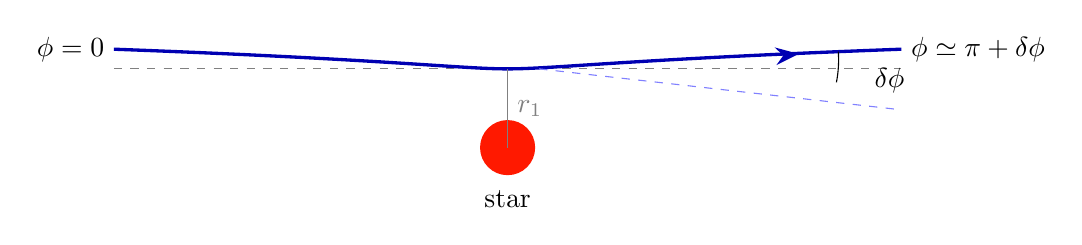
\begin{tikzpicture}[scale=1.0,>=Stealth]
  \fill[red!80!orange] (0,0) circle (0.35);
  \node at (0,-0.65) {star};
  \draw[dashed,gray] (-5,1.0) -- (5,1.0);
  \draw[very thick,blue!70!black] (-5,1.25) .. controls (-1.5,1.12) and (-0.6,1.0) .. (0,1.0) .. controls (0.6,1.0) and (1.5,1.12) .. (5,1.25);
  \draw[->,very thick,blue!70!black] (3.6,1.18) -- (3.7,1.19);
  \draw[gray,thin] (0,0) -- (0,1.0) node[midway,right] {$r_1$};
  \draw[dashed,blue!50] (0.4,1.0) -- (5,0.48);
  \draw (4.2,1.22) arc (4:-11:1.5);
  \node at (4.85,0.85) {$\delta\phi$};
  \node[left] at (-5,1.25) {$\phi=0$};
  \node[right] at (5,1.25) {$\phi\simeq\pi+\delta\phi$};
\end{tikzpicture}
\caption{Bending of light by a star: a photon coming from $r\to\infty$ at $\phi=0$ reaches the closest distance $r_1$ and leaves towards $\phi=\pi+\delta\phi$ instead of $\phi=\pi$. The deflection angle is $\delta\phi=2\rs/r_1$ (strongly exaggerated in the figure).}
\label{fig:bending}
\end{figure}

\paragraph{Consequence: gravitational lensing.} Light from a distant source (galaxy, quasar) passing near a massive object (galaxy, cluster) is deflected towards it; an observer on Earth can see multiple, distorted or magnified images of the source (Einstein rings, arcs) (\cref{fig:lensing}).

\begin{figure}[ht]
\centering
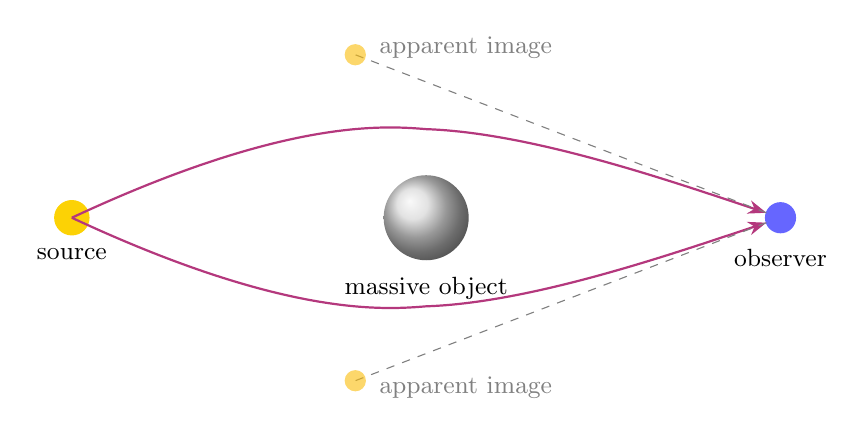
\begin{tikzpicture}[scale=0.9,>=Stealth]
  \fill[yellow!70!orange] (-5,0) circle (0.25); \node[below] at (-5,-0.3) {\small source};
  \shade[ball color=gray!30] (0,0) circle (0.6); \node[below] at (0,-0.7) {\small massive object};
  \fill[blue!60] (5,0) circle (0.22); \node[below] at (5,-0.3) {\small observer};
  \draw[thick,magenta!70!black,->] (-5,0) .. controls (-2,1.4) and (-0.6,1.3) .. (0,1.25) .. controls (1.5,1.2) and (3.5,0.5) .. (4.8,0.07);
  \draw[thick,magenta!70!black,->] (-5,0) .. controls (-2,-1.4) and (-0.6,-1.3) .. (0,-1.25) .. controls (1.5,-1.2) and (3.5,-0.5) .. (4.8,-0.07);
  \draw[dashed,gray] (4.8,0.07) -- (-1,2.3); \draw[dashed,gray] (4.8,-0.07) -- (-1,-2.3);
  \fill[yellow!50!orange,opacity=0.6] (-1,2.3) circle (0.15); \fill[yellow!50!orange,opacity=0.6] (-1,-2.3) circle (0.15);
  \node[gray,right] at (-0.8,2.4) {\small apparent image};
  \node[gray,right] at (-0.8,-2.4) {\small apparent image};
\end{tikzpicture}
\caption{Gravitational lensing: rays from a distant source bend around a massive object, and the observer sees apparent images of the source in the directions from which the rays arrive.}
\label{fig:lensing}
\end{figure}

\section{Complement: precession of the perihelion of Mercury}

For a massive particle, $\mathcal L=c^2$ with $\lambda=\tau$, and the conserved quantities are $(1-\rs/r)\dot t=\gamma$, $r^2\dot\phi=J$. The same steps as above give, with $u=1/r$,
\[
  \Big(\frac{\dd u}{\dd\phi}\Big)^2=\frac{c^2(\gamma^2-1)}{J^2}+\frac{c^2\rs}{J^2}u-u^2+\rs u^3 .
\]
Differentiating with respect to $\phi$ and dividing by $2\,\dd u/\dd\phi$ gives the orbit equation
\begin{equation}
  \frac{\dd^2u}{\dd\phi^2}+u=\frac{\GN M}{J^2}+\frac{3\GN M}{c^2}u^2 .
\end{equation}
Without the last term this is the Newtonian (Binet) equation, whose solution is the closed ellipse $u_0=\frac{\GN M}{J^2}(1+e\cos\phi)$. The relativistic term $3\GN Mu^2/c^2$ is a tiny perturbation: inserting $u_0$ in it, the only term that accumulates over many orbits is the resonant one, $\frac{6\GN^2M^2}{c^2J^2}\cdot\frac{\GN M}{J^2}\,e\cos\phi$, which yields $u\simeq\frac{\GN M}{J^2}\big[1+e\cos\big((1-\epsilon)\phi\big)\big]$ with $\epsilon=3\GN^2M^2/(c^2J^2)$. The perihelion is reached when $(1-\epsilon)\phi=2\pi n$: it advances by
\begin{equation}
  \delta\phi_{\rm per}\simeq2\pi\epsilon=\frac{6\pi\GN M}{c^2a(1-e^2)}\ \text{per orbit},
\end{equation}
using $J^2=\GN Ma(1-e^2)$ ($a$ the semi-major axis, $e$ the eccentricity). For Mercury this gives $43''$ per century, exactly the anomalous precession that Newtonian gravity (including perturbations from the other planets) could not explain. The orbit is no longer a closed ellipse but a rosette (\cref{fig:mercury}).

\begin{figure}[ht]
\centering
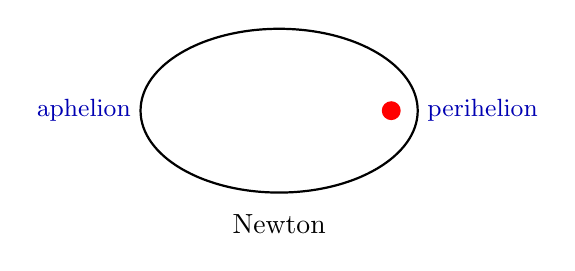
\begin{tikzpicture}[scale=0.8]
  \draw[thick] (0,0) ellipse (2.2 and 1.3);
  \fill[red] (1.78,0) circle (0.15);
  \node[blue!70!black,right,font=\small] at (2.2,0) {perihelion};
  \node[blue!70!black,left,font=\small] at (-2.2,0) {aphelion};
  \node at (0,-1.8) {Newton};
\end{tikzpicture}
\hspace{1.5cm}
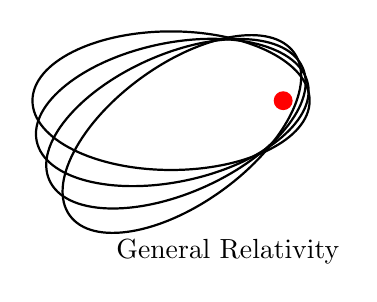
\begin{tikzpicture}[scale=0.8]
  \foreach \a in {0,12,24,36}{\draw[thick,rotate around={\a:(0,0)}] (-0.9,0) ellipse (2.2 and 1.1);}
  \fill[red] (0.88,0) circle (0.15);
  \node at (0,-2.4) {General Relativity};
\end{tikzpicture}
\caption{Left: in Newtonian gravity, a bound orbit is a closed ellipse with the Sun at one focus. Right: in GR the ellipse slowly precesses (the effect is enormously exaggerated here): the perihelion advances at each revolution.}
\label{fig:mercury}
\end{figure}

\section{The classic tests of General Relativity}
\begin{enumerate}[label=(\roman*),nosep]
\item Bending of light (\cref{sec:light-bending}).
\item Precession of the perihelion of Mercury.
\item Shapiro effect (time delay of radar signals passing near the Sun): see Problem Sheet 4, where one finds the maximal delay $\delta t_{\max}=\frac{4\GN M_\odot}{c^3}\big[1+\ln\frac{4r_Ar_B}{R_\odot^2}\big]$.
\item (Gravitational redshift, which already follows from the Equivalence Principle.)
\end{enumerate}

% =====================================================================
\chapter{Black holes}\label{ch:blackholes}
% =====================================================================

We now consider the singularities of the Schwarzschild metric,
\[
  c^2\dd\tau^2=\Big(1-\frac\rs r\Big)c^2\dd t^2-\Big(1-\frac\rs r\Big)^{-1}\dd r^2-r^2\dd\Omega^2 :
\]
\begin{itemize}[nosep]
\item $r=0$ is a \textbf{genuine} (physical, curvature) singularity: it cannot be avoided by a change of coordinates. Indeed the curvature invariant $R_{\mu\nu\rho\sigma}R^{\mu\nu\rho\sigma}=12\rs^2/r^6$ (a scalar!) diverges there. It is, however, not ``naked'' (see below).
\item $r=\rs$ is only an \textbf{apparent} (coordinate) singularity: it can be removed by a change of coordinates. All curvature invariants are finite there; the problem is that the Schwarzschild coordinates are ill-behaved. At $r=\rs$ the $t$ coordinate changes from time-like to space-like.
\end{itemize}

\section{Radial light rays}

Let us consider radially moving photons ($\theta,\phi=$ const). Such photons move in a space-time
\[
  c^2\Big(1-\frac\rs r\Big)\dd t^2-\frac{\dd r^2}{1-\rs/r}=0\qquad\Longrightarrow\qquad
  \begin{cases}c\,\dd t=+\dfrac{\dd r}{1-\rs/r}&\text{(outgoing)},\\[1.5ex] c\,\dd t=-\dfrac{\dd r}{1-\rs/r}&\text{(incoming)}.\end{cases}
\]
Integrating, with $\int\frac{\dd r}{1-\rs/r}=\int\frac{r\,\dd r}{r-\rs}=\int\Big(1+\frac{\rs}{r-\rs}\Big)\dd r=r+\rs\ln\Big|\frac r\rs-1\Big|+\text{const}$, we get
\begin{equation}
  \begin{cases} ct=r+\rs\ln\left|\dfrac r\rs-1\right|+C &\text{(outgoing)},\\[1.5ex] -ct=r+\rs\ln\left|\dfrac r\rs-1\right|+D &\text{(incoming)},\end{cases}
\end{equation}
with $C,D$ integration constants (labelling the different light rays). The combination $r_*\equiv r+\rs\ln|r/\rs-1|$ is called the \emph{tortoise coordinate}. As $r\to\rs$, $r_*\to-\infty$: an incoming light ray needs an infinite coordinate time $t$ to reach $r=\rs$. This is a hint that $t$ is a bad coordinate there.

\section{Kruskal--Szekeres coordinates}

We now switch to the Kruskal--Szekeres coordinates $U,V$, defined such that the two families of light rays are the coordinate lines:
\begin{equation}
  UV=e^{(C+D)/2\rs}\to e^{r/\rs}\Big(\frac r\rs-1\Big),\qquad
  \pm\frac VU=e^{(C-D)/2\rs}\to e^{ct/\rs},
  \label{eq:kruskal}
\end{equation}
with the sign $+$ for $r>\rs$ and $-$ for $r<\rs$. Explicitly, for $r>\rs$: $V=e^{(ct+r_*)/2\rs}$, $U=e^{(r_*-ct)/2\rs}$. Along an outgoing ray $ct-r_*=C$, so $U=e^{-C/2\rs}$ is constant; along an incoming ray $ct+r_*=-D$, so $V=e^{-D/2\rs}$ is constant. Note: $r=\rs\Leftrightarrow V=0$ or $U=0$.

\paragraph{The metric in the new coordinates.} Focus first on $r>\rs$ (e.g.\ an incoming photon).
\begin{enumerate}[label=(\roman*)]
\item $\dd(UV)=V\dd U+U\dd V=UV\Big(\dfrac{\dd V}V+\dfrac{\dd U}U\Big)$, and on the other hand
\begin{align*}
  \dd(UV)&=\dd\Big[e^{r/\rs}\Big(\frac r\rs-1\Big)\Big]=e^{r/\rs}\Big[\frac1\rs+\frac1\rs\Big(\frac r\rs-1\Big)\Big]\dd r=e^{r/\rs}\frac{r}{\rs^2}\dd r\\
  &=\frac{UV}{\frac r\rs-1}\frac{r}{\rs^2}\dd r=\frac{UV\,\dd r}{\rs(1-\rs/r)}.\quad(1)
\end{align*}
\item $\dd\Big(\dfrac VU\Big)=\dfrac1U\dd V-\dfrac V{U^2}\dd U=\dfrac VU\Big(\dfrac{\dd V}V-\dfrac{\dd U}U\Big)$, and on the other hand $\dd\big(e^{ct/\rs}\big)=e^{ct/\rs}\dfrac{c\,\dd t}{\rs}=\dfrac VU\dfrac{c\,\dd t}{\rs}$.\quad(2)
\end{enumerate}
Using (1) and (2):
\begin{equation}
  \frac{\dd V}V+\frac{\dd U}U=\frac{\dd r}{\rs(1-\rs/r)},\qquad\frac{\dd V}V-\frac{\dd U}U=\frac{c\,\dd t}{\rs}.
\end{equation}
Replacing these differential relations back into the radial part of $\dd s^2$:
\begin{align}
  \dd s^2\big|_{\rm radial}&=\Big(1-\frac\rs r\Big)\Big[c^2\dd t^2-\frac{\dd r^2}{(1-\rs/r)^2}\Big]
  =\Big(1-\frac\rs r\Big)\rs^2\Big[\Big(\frac{\dd V}V-\frac{\dd U}U\Big)^2-\Big(\frac{\dd V}V+\frac{\dd U}U\Big)^2\Big]\nonumber\\
  &=-4\rs^2\Big(1-\frac\rs r\Big)\frac{\dd U\,\dd V}{UV}
  =-4\rs^2\,\frac{r-\rs}{r}\,\frac{\rs\,e^{-r/\rs}}{r-\rs}\,\dd U\,\dd V ,
\end{align}
using $(a-b)^2-(a+b)^2=-4ab$ and $UV=e^{r/\rs}(r-\rs)/\rs$. Hence
\begin{keyresult}[Schwarzschild metric in Kruskal--Szekeres coordinates]
\begin{equation}
  \dd s^2=-\frac{4\rs^3}{r}e^{-r/\rs}\,\dd U\,\dd V-r^2\dd\Omega^2,\qquad UV=\Big(\frac r\rs-1\Big)e^{r/\rs}.
\end{equation}
This is \textbf{non-singular at $r=\rs$}: $r=\rs$ was only a coordinate singularity, which we have avoided with this coordinate transformation. The only singularity left is at $r=0$.
\end{keyresult}

\paragraph{Comments.}
\begin{itemize}
\item For a given point $(U,V)$, $r$ can be computed from $UV=(r/\rs-1)e^{r/\rs}$ (the right-hand side is a monotonic function of $r$).
\item The derivation used $r>\rs$, but the final expression is analytic in $U,V$ and can be extended to $r<\rs$ (with the sign $-$ in \eqref{eq:kruskal}): it is the analytic continuation of the metric.
\item For a photon initially at $r>\rs$ to reach $r<\rs$, either $V$ or $U$ has to change sign: for $r>\rs$ both $V>0$ and $U>0$, while $r<\rs\Leftrightarrow UV<0$.
\end{itemize}

\section{The Kruskal diagram}

\textbf{Goal:} draw the Schwarzschild coordinates in the $(U,V)$ plane. It is customary to draw $V$ and $U$ along the two diagonals, so that the ``time'' $T\propto V-U$ points upwards and the ``space'' $X\propto V+U$ to the right (\cref{fig:kruskal}). Reminder: $UV=e^{r/\rs}(r/\rs-1)$ and $\pm V/U=e^{ct/\rs}$ ($+$ for $r>\rs$, $-$ for $r<\rs$).
\begin{enumerate}
\item If $V=0$ or $U=0$, then $UV=0\Rightarrow r=\rs$: both axes are the surface $r=\rs$.
\item If $V=0$: $V/U=0=e^{ct/\rs}\Rightarrow t\to-\infty$ along the $U$ axis. If $U=0$: $V/U=\infty=e^{ct/\rs}\Rightarrow t\to+\infty$ along the $V$ axis.
\item Lines of $t=$ const: $V/U=$ const, i.e.\ $V=\text{const}\times U$: \textbf{straight lines through the origin}.
\item Lines of $r=$ const $>\rs$: $UV=$ const $>0$: \textbf{hyperbolas} in the first quadrant ($U,V>0$, the right wedge of the figure).
\item $r=0$: $UV=-1$, a hyperbola in the region $U<0<V$ (top wedge) --- and its mirror image in the region $V<0<U$ (bottom wedge).
\end{enumerate}
\begin{itemize}
\item The first quadrant ($U,V>0$) corresponds to $r>\rs$ and $-\infty<t<\infty$: full coverage of the $r>\rs$ space-time of Schwarzschild (region I).
\item Radial photons: $\dd s^2=0\Rightarrow\dd U\,\dd V=0\Rightarrow V=$ const (incoming) or $U=$ const (outgoing): straight lines at $45^\circ$ in the diagram, as in Minkowski space. Light cones are oriented upwards everywhere and they do not change orientation (unlike in Schwarzschild coordinates, where they ``close up'' as $r\to\rs$): \emph{the Kruskal diagram is a good map of the causal structure}.
\item A stationary (static) observer at $r>\rs$ moves along a hyperbola $r=$ const in region I. He/she does not have access beyond the first quadrant; in particular he/she never receives signals from $r\le\rs$ ($UV\le0$).
\item The top wedge ($U<0<V$, $0<r<\rs$, region II) is the \textbf{black hole} interior: once inside, every future-directed time-like or null curve ends on the singularity $r=0$. The line $U=0$ ($r=\rs$, $t=+\infty$) is the \textbf{event horizon}: a one-way membrane. (The bottom wedge is a ``white hole'' and the left wedge a second asymptotic region; they are part of the maximal analytic extension of the \emph{eternal} Schwarzschild solution but are absent for a black hole formed by collapse.)
\end{itemize}

\begin{figure}[ht]
\centering
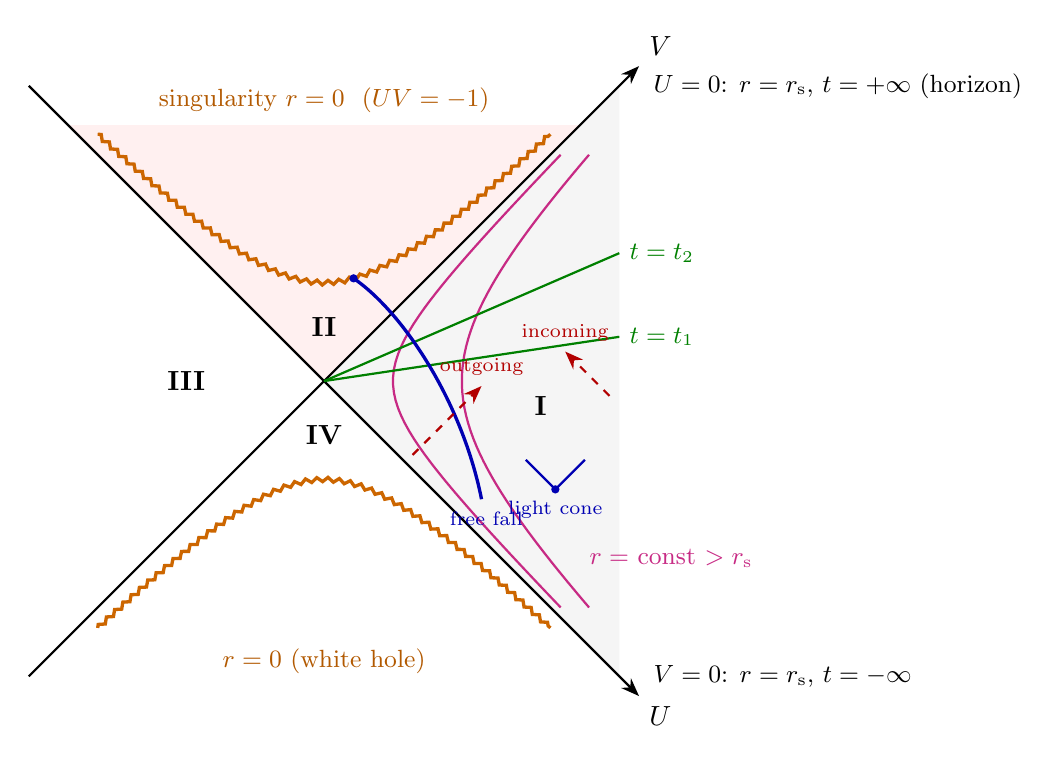
\begin{tikzpicture}[scale=1.25,>=Stealth]
  \fill[gray!8] (0,0) -- (3.0,3.0) -- (3.0,-3.0) -- cycle;
  \fill[red!6] (0,0) -- (-2.6,2.6) -- (2.6,2.6) -- cycle;
  \draw[->,thick] (-3,-3) -- (3.2,3.2) node[above right] {$V$};
  \draw[->,thick] (-3,3) -- (3.2,-3.2) node[below right] {$U$};
  \draw[very thick,orange!80!black,decorate,decoration={zigzag,amplitude=0.8pt,segment length=4pt},domain=-2.3:2.3,samples=60] plot (\x,{sqrt(1+\x*\x)});
  \draw[very thick,orange!80!black,decorate,decoration={zigzag,amplitude=0.8pt,segment length=4pt},domain=-2.3:2.3,samples=60] plot (\x,{-sqrt(1+\x*\x)});
  \node[orange!70!black,fill=white,inner sep=1pt] at (0,2.85) {\small singularity $r=0$ \ ($UV=-1$)};
  \node[orange!70!black,fill=white,inner sep=1pt] at (0,-2.85) {\small $r=0$ (white hole)};
  \foreach \a in {0.7,1.4}{\draw[thick,magenta!80!black,domain=-2.3:2.3,samples=60] plot ({sqrt(\a*\a+\x*\x)},\x);}
  \node[magenta!80!black,right] at (2.6,-1.8) {\small $r=$ const $>\rs$};
  \draw[thick,green!50!black] (0,0) -- (3.0,1.3) node[right] {\small $t=t_2$};
  \draw[thick,green!50!black] (0,0) -- (3.0,0.45) node[right] {\small $t=t_1$};
  \node[right,font=\small] at (3.25,3.0) {$U=0$: $r=\rs$, $t=+\infty$ (horizon)};
  \node[right,font=\small] at (3.25,-3.0) {$V=0$: $r=\rs$, $t=-\infty$};
  \node at (2.2,-0.25) {\bf I};
  \node at (0,0.55) {\bf II};
  \node at (-1.4,0) {\bf III};
  \node at (0,-0.55) {\bf IV};
  \begin{scope}[shift={(2.35,-1.1)}]
    \draw[blue!70!black,thick] (-0.3,0.3) -- (0,0) -- (0.3,0.3);
    \fill[blue!70!black] (0,0) circle (1.2pt);
    \node[blue!70!black,font=\scriptsize,below] at (0,-0.02) {light cone};
  \end{scope}
  \draw[very thick,blue!70!black] (1.6,-1.2) .. controls (1.4,-0.2) and (0.8,0.7) .. (0.3,1.044);
  \fill[blue!70!black] (0.3,1.044) circle (1.2pt);
  \node[blue!70!black,font=\scriptsize] at (1.65,-1.4) {free fall};
  \draw[->,red!70!black,thick,dashed] (0.9,-0.75) -- (1.6,-0.05) node[above,font=\scriptsize] {outgoing};
  \draw[->,red!70!black,thick,dashed] (2.9,-0.15) -- (2.45,0.3) node[above,font=\scriptsize] {incoming};
\end{tikzpicture}
\caption{The Kruskal diagram. The axes $U=0$ and $V=0$ are the surface $r=\rs$. Region I ($U,V>0$) is the exterior $r>\rs$, covered by Schwarzschild coordinates: lines of constant $t$ are straight lines through the origin (green) and lines of constant $r$ are hyperbolas (magenta). Region II is the black-hole interior, bounded by the singularity $r=0$ ($UV=-1$, zigzag). Radial light rays are lines at $45^\circ$ ($U$ or $V$ constant) and light cones keep their orientation. A freely-falling observer crosses the horizon $U=0$ in finite proper time and ends at $r=0$.}
\label{fig:kruskal}
\end{figure}

\section{A freely-falling observer}

Consider an observer falling radially ($\theta,\phi=$ const) from rest at infinity. The Lagrangian (with $\lambda=\tau$) is
\[
  \mathcal L=c^2\Big(1-\frac\rs r\Big)\dot t^2-\Big(1-\frac\rs r\Big)^{-1}\dot r^2=c^2 .
\]
$t$ is cyclic: $\big(1-\frac\rs r\big)\dot t=\gamma$ (constant). Inserting in $\mathcal L=c^2$: $\frac{c^2\gamma^2-\dot r^2}{1-\rs/r}=c^2$, i.e.
\[
  \gamma=\sqrt{\Big(1-\frac{\rs}{r}\Big)+\frac{\dot r^2}{c^2}} .
\]
Boundary condition: $\dot r=0$ at $r\to\infty$ (at rest at infinity) $\Rightarrow\gamma=1$. Hence
\begin{equation}
  \dot r^2=\frac{\rs c^2}{r},\qquad\dot t=\frac{1}{1-\rs/r}.
\end{equation}
(The first equation is formally identical to the Newtonian energy conservation $\frac12\dot r^2-\frac{\GN M}{r}=0$, but with proper time.)

\paragraph{Proper time.} We define $x$ by $r=\rs x^2$ (so $\dd r=2\rs x\,\dd x$). For infall $\dot r=-c\sqrt{\rs/r}=-c/x$, so $2\rs x\,\dd x=-\frac cx\dd\tau$, i.e.\ $c\,\dd\tau=-2\rs x^2\dd x$ and
\begin{equation}
  c(\tau_0-\tau)=\frac23\rs x^3=\frac23\frac{r^{3/2}}{\rs^{1/2}},
\end{equation}
where $\tau_0$ is the proper time at which the observer reaches $r=0$ ($x$ tracks the proper time; everything chosen for $\gamma=1$). In particular, the proper time needed to go from $r=\rs$ ($x=1$) to $r=0$ is \emph{finite}: $\Delta\tau=\frac{2\rs}{3c}$. Nothing special happens to the falling observer at the horizon.

\paragraph{Coordinate time: a static observer at $r>\rs$ watching the free fall.} From the $t$ equation, $\dd t=\frac{\dd\tau}{1-\rs/r}=\frac{x^2}{x^2-1}\dd\tau$, so
\[
  c\,\dd t=-\frac{2\rs x^4\,\dd x}{x^2-1}=-2\rs\Big(x^2+1+\frac{1}{x^2-1}\Big)\dd x ,
\]
and integrating (with $\int\frac{\dd x}{x^2-1}=\frac12\ln\big|\frac{x-1}{x+1}\big|$):
\begin{equation}
  ct=-\rs\left[\frac23x^3+2x+\ln\left|\frac{x-1}{x+1}\right|\right]+\text{const}.
\end{equation}
\begin{enumerate}[label=(\roman*)]
\item For $x\to\infty$ (far away), $ct\simeq-\frac23\rs x^3+\dots$: $\tau$ and $t$ agree qualitatively.
\item For $x\to1$, i.e.\ $r\to\rs$: $c\tau\to c\tau_0-\frac23\rs$ is finite, while $\ln|x-1|\to-\infty$, so $t\to+\infty$ \textbf{diverges}.
\end{enumerate}
The falling observer actually falls (and crosses the horizon in a finite proper time), but for the external (static) observer, who never sees him/her getting there, the image freezes at $r=\rs$, while becoming more and more redshifted.

\begin{keyresult}
For an external observer, $r=0$ (and indeed the whole region $r\le\rs$) is inaccessible: the singularity is hidden behind the event horizon. GR (with physically reasonable matter) does not seem to produce \textbf{naked singularities} (Penrose's \emph{cosmic censorship conjecture}).
\end{keyresult}

% =====================================================================
\chapter{Cosmology and the FLRW metric}\label{ch:cosmology}
% =====================================================================

We want to build an \emph{average} metric for the Universe as a whole, on scales much larger than galaxies and clusters of galaxies.

\section{The cosmological principle}

The fundamental assumptions of standard cosmology are:
\begin{enumerate}
\item \textbf{Copernican principle:} we do not occupy a special place; the Universe looks the same at any spatial point: it is \textbf{homogeneous}.
\item The Universe looks the same in all directions, no matter in which direction we are looking: it is \textbf{isotropic}.
\end{enumerate}
Combining (1) and (2) we have the \textbf{cosmological principle}:
\begin{keyresult}[Cosmological principle]
The Universe is homogeneous and isotropic (on large scales).
\end{keyresult}
These statements refer to \emph{space}, not to space-time: the Universe is ``spatially'' homogeneous and isotropic, but it can evolve in time. (Isotropy around every point implies homogeneity; observationally, isotropy is strongly supported by the cosmic microwave background, which is isotropic to one part in $10^5$.)

\textbf{Goal:} constrain the metric to incorporate the cosmological principle, and describe an expanding Universe. The result is the Friedmann--Lemaître--Robertson--Walker (FLRW) metric.

\section{Construction of the FLRW metric}

\subsection{Isotropy}
Isotropy is, more or less, a spherical symmetry around every point. Start with ``isotropic'' coordinates, which we denote by $(ct,x,y,z)$, and impose that:
\begin{enumerate}[nosep]
\item the symmetry has its origin at $x=y=z=0$;
\item the 3D line element $\dd l^2$ only depends on time and on the distance from the origin:
\begin{equation}
  \dd l^2=g\big(t,\sqrt{x^2+y^2+z^2}\big)\,\dd x^i\dd x^i ,
\end{equation}
where $\sqrt{x^2+y^2+z^2}$ is \emph{not} the proper distance from the origin, just a coordinate distance.
\end{enumerate}
Let us switch to ``spherical'' coordinates $(t,r,\theta,\phi)$, with $x=r\sin\theta\cos\phi$, $y=r\sin\theta\sin\phi$, $z=r\cos\theta$. In these coordinates
\begin{equation}
  \dd l^2=g(t,r)\big(\dd r^2+r^2\dd\theta^2+r^2\sin^2\theta\,\dd\phi^2\big).
\end{equation}
Let us include $t$. For $\dd t\neq0$ we demand $\dd s^2$ to be invariant under $\theta\to-\theta$ and $\phi\to-\phi$ (isotropy); since $g_{\mu\nu}$ is a $(0,2)$ tensor, exactly as for Schwarzschild this implies $g_{t\theta}=g_{t\phi}=0$. The line element reads
\[
  \dd s^2=f(t,r)c^2\dd t^2-g(t,r)\dd r^2+h(t,r)\,\dd t\,\dd r-g(t,r)r^2\big(\dd\theta^2+\sin^2\theta\,\dd\phi^2\big),
\]
where $f,g,h$ are unknown functions.

\paragraph{The cross term $h(t,r)\,\dd t\,\dd r$} is a weird (``annoying'') term, but it can be eliminated through an appropriate coordinate transformation. \emph{Why?} Consider the example $\dd s^2=A\,\dd t^2-B\,\dd r^2+2C\,\dd r\,\dd t$ (with $A,B,C$ functions of $t,r$), and introduce a new time $T(t,r)\equiv t+\psi(r)$. Then $\dd T=\dd t+\psi'\dd r$ and
\[
  A\,\dd T^2=A\,\dd t^2+2A\psi'\,\dd t\,\dd r+A\psi'^2\dd r^2\ \Longrightarrow\
  A\,\dd t^2+2C\,\dd t\,\dd r=A\,\dd T^2+2(C-A\psi')\,\dd t\,\dd r-A\psi'^2\dd r^2 .
\]
Choosing $\psi$ such that $\frac{\dd\psi}{\dd r}=\frac CA$ (if $A,C$ depend on $t$, one uses a slightly more general $T(t,r)$ with an integrating factor), the cross term disappears. Basically, we can choose $C=0$, i.e.\ $h(t,r)=0$ (see e.g.\ Hobson, Efstathiou \& Lasenby for the general proof). We are left with
\begin{equation}
  \dd s^2=f(t,r)c^2\dd t^2-g(t,r)\big[\dd r^2+r^2\dd\theta^2+r^2\sin^2\theta\,\dd\phi^2\big].
\end{equation}

\subsection{Homogeneity}
\paragraph{The spatial part.} Consider three objects (e.g.\ galaxies) forming a triangle in space, on the hypersurface $t=0$, and look at the same three objects at a later time, e.g.\ on the hypersurface $t=1$ (\cref{fig:triangles}).
\begin{itemize}
\item \textbf{Isotropy} imposes that the two triangles must be \emph{similar}: an expansion which stretches one direction more than another (anisotropic expansion) is not permitted, as it would single out a preferred direction.
\item \textbf{Homogeneity} imposes that the magnification factor must be the same in a different patch of space.
\end{itemize}
Hence the time dependence of $g$ must factorise into a universal, position-independent factor:
\begin{equation}
  g(t,r)=a^2(t)\,h(r),\qquad a^2(t)>0
\end{equation}
($h$ here is a new function, not the same as before).

\begin{figure}[ht]
\centering
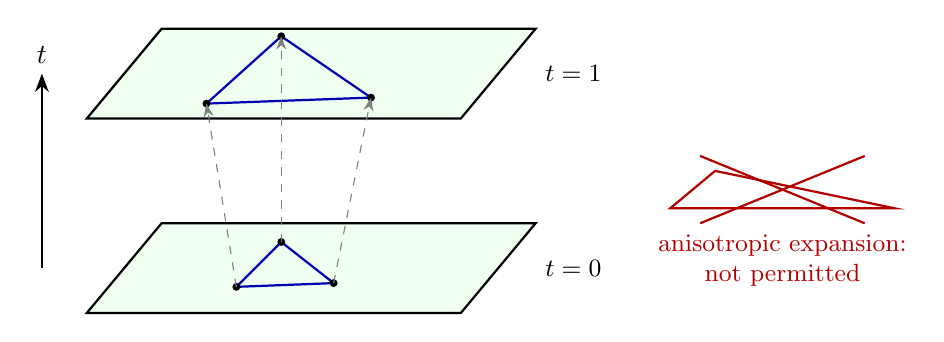
\begin{tikzpicture}[scale=0.95,>=Stealth]
  % hypersurface t=0
  \draw[thick,fill=green!6] (0,0) -- (5,0) -- (6,1.2) -- (1,1.2) -- cycle;
  \node[right] at (6.0,0.6) {\small $t=0$};
  \coordinate (A) at (2.0,0.35); \coordinate (B) at (3.3,0.4); \coordinate (C) at (2.6,0.95);
  \draw[thick,blue!70!black] (A) -- (B) -- (C) -- cycle;
  \foreach \p in {A,B,C} \fill (\p) circle (1.5pt);
  % hypersurface t=1
  \draw[thick,fill=green!6] (0,2.6) -- (5,2.6) -- (6,3.8) -- (1,3.8) -- cycle;
  \node[right] at (6.0,3.2) {\small $t=1$};
  \coordinate (A1) at (1.6,2.8); \coordinate (B1) at (3.8,2.88); \coordinate (C1) at (2.6,3.7);
  \draw[thick,blue!70!black] (A1) -- (B1) -- (C1) -- cycle;
  \foreach \p in {A1,B1,C1} \fill (\p) circle (1.5pt);
  \foreach \p/\q in {A/A1,B/B1,C/C1} \draw[gray,dashed,->] (\p) -- (\q);
  \draw[->,thick] (-0.6,0.6) -- (-0.6,3.2) node[above] {$t$};
  % not permitted
  \begin{scope}[shift={(7.8,1.4)}]
    \draw[thick,red!70!black] (0,0) -- (3.0,0) -- (0.6,0.5) -- cycle;
    \node[red!70!black,font=\small,align=center] at (1.5,-0.7) {anisotropic expansion:\\ not permitted};
    \draw[red!70!black,thick] (0.4,-0.2) -- (2.6,0.7) (0.4,0.7) -- (2.6,-0.2);
  \end{scope}
\end{tikzpicture}
\caption{Isotropy and homogeneity. Three galaxies form a triangle on the hypersurface $t=0$; at a later time ($t=1$) isotropy imposes that the triangle be \emph{similar} to the original one (a uniform magnification), and homogeneity that the magnification be the same everywhere. A stretched (anisotropic) triangle is not permitted.}
\label{fig:triangles}
\end{figure}

\paragraph{The $\dd t^2$ part.} Homogeneity implies that any ``static'' observer (one at fixed spatial coordinates) must measure the same time. If $f$ depended on $r$, two observers at different radii $r_1,r_2$ would measure different proper times between the same two hypersurfaces $t_1,t_2$, which would distinguish the two locations: the space would be inhomogeneous. Hence $f$ can only depend on $t$, $f=f(t)$. We can then perform a coordinate transformation (called ``\emph{synchronisation}'')
\[
  \dd t\ \to\ \dd t'=\sqrt{f(t)}\,\dd t,
\]
after which $g_{00}=1$, and (dropping the primes)
\begin{equation}
  \dd s^2=c^2\dd t^2-a^2(t)\,h(r)\big[\dd r^2+r^2\dd\theta^2+r^2\sin^2\theta\,\dd\phi^2\big].
\end{equation}
Next we perform a coordinate transformation to remove $h(r)$ from the angular part: $r\to\tilde r(r)$ with $\tilde r^2=h(r)r^2$. Then
\begin{equation}
  \dd s^2=c^2\dd t^2-a^2(t)\,g(\tilde r)\,\dd\tilde r^2-a^2(t)\,\tilde r^2\big[\dd\theta^2+\sin^2\theta\,\dd\phi^2\big],
\end{equation}
for some new function $g(\tilde r)$; $\tilde r$ still has a radius interpretation (the spheres $\tilde r=$ const have area $4\pi a^2\tilde r^2$). We drop the tilde in the following.

\subsection{Constant spatial curvature}
Ignoring $a^2(t)$ (i.e.\ at fixed $t$), homogeneity implies that the \textbf{scalar curvature $R_3$ of 3-space must be constant} (it is a scalar, and all points are equivalent).

The spatial part, $\dd l^2=g(r)\dd r^2+r^2\dd\Omega^2$, has the same generic form as the Schwarzschild spatial metric, so we can recycle the results of \cref{ch:schwarzschild}: setting $A=$ const in the static spherically symmetric metric (so that $\dd s^2=\dd t^2-\dd l^2$), the 4D Ricci scalar computed from \eqref{eq:ricci-static} is $R=R^t{}_t+R^r{}_r+2R^\theta{}_\theta=-\big[\frac{2B'}{rB^2}+\frac{2(B-1)}{r^2B}\big]$, and for such a product metric it equals minus the scalar curvature of the (positive-definite) 3-metric. With $B\to g$:
\begin{equation}
  R_3=\frac{2g'}{rg^2}+\frac{2(g-1)}{r^2g}\overset{!}{=}6k,\qquad k\in\R ,
\end{equation}
(the normalisation $6k$ is chosen for later convenience; for a 3-sphere of radius $a_0$, $R_3=6/a_0^2$). Solving: set $y\equiv1/g$, so that $g'/g^2=-y'$:
\[
  -\frac{2y'}{r}+\frac{2(1-y)}{r^2}=6k\ \Longrightarrow\ -ry'+1-y=3kr^2\ \Longrightarrow\ \frac{\dd}{\dd r}(ry)=1-3kr^2\ \Longrightarrow\ ry=r-kr^3+C ,
\]
i.e.
\[
  g(r)=\frac{1}{1-kr^2+C/r}.
\]
\textbf{Boundary condition:} $g\to1$ as $r\to0$ (local flatness: space must look Euclidean around the origin, which is like any other point), hence $C=0$ and $g(r)=\frac{1}{1-kr^2}$.

\begin{keyresult}[The FLRW metric]
\begin{equation}
  \dd s^2=c^2\dd t^2-a^2(t)\left[\frac{\dd r^2}{1-kr^2}+r^2\dd\theta^2+r^2\sin^2\theta\,\dd\phi^2\right].
\end{equation}
This is the \textbf{Friedmann--Lemaître--Robertson--Walker} (FLRW) metric.
\end{keyresult}

\section{Remarks}
\begin{enumerate}[label=(\roman*)]
\item In principle $k\in\R$. However, it is always possible to rescale $r$ (and $a$ correspondingly: $r\to\lambda r$, $a\to a/\lambda$, $k\to k/\lambda^2$) in order to obtain $k=0,\pm1$.
\item A Universe is called
\begin{itemize}[nosep]
\item \textbf{closed} if $k=+1$: it has a finite volume;
\item \textbf{open} (hyperbolic) if $k=-1$: infinite volume;
\item \textbf{flat} if $k=0$: infinite volume. Careful: \emph{not} a flat space-time! The space-time is flat if and only if $k=0$ and $a(t)=$ const.
\end{itemize}
\item The Ricci scalar of FLRW is (with $c=1$)
\begin{equation}
  R=-6\left[\frac{\ddot a}{a}+\frac{\dot a^2}{a^2}+\frac{k}{a^2}\right]
\end{equation}
with our sign conventions (with the conventions used in the lecture, or in the signature $(-,+,+,+)$, it reads $R=+6[\dots]$). If $a\to0$, $R$ diverges: this is a genuine singularity (the Big Bang). Conventionally, $a=1$ today.
\item $a(t)$ is called the \textbf{scale factor}.
\item One can write the spatial part of $g_{\mu\nu}$ in a more geometric way by setting
\[
  r=\begin{cases}\sin\chi,&k=+1,\\ \chi,&k=0,\\ \sinh\chi,&k=-1,\end{cases}
\]
giving
\[
  \dd l^2=\begin{cases}\dd\chi^2+\sin^2\!\chi\,(\dd\theta^2+\sin^2\theta\,\dd\phi^2)&\text{3-sphere},\\
  \dd\chi^2+\chi^2(\dd\theta^2+\sin^2\theta\,\dd\phi^2)&\text{Euclidean},\\
  \dd\chi^2+\sinh^2\chi\,(\dd\theta^2+\sin^2\theta\,\dd\phi^2)&\text{hyperbolic (``saddle'')}.\end{cases}
\]
(Check for $k=1$: $\dd r=\cos\chi\,\dd\chi$ and $1-r^2=\cos^2\chi$, so $\dd r^2/(1-r^2)=\dd\chi^2$; for general $k>0$, $r=\sin(\sqrt k\chi)/\sqrt k$.)
\end{enumerate}

\section{Comoving observers}

It is possible to show that any world-line with $\chi,\theta,\phi=$ const (equivalently $r,\theta,\phi=$ const) is a \textbf{geodesic}, and that along it $t=\tau$. Indeed, since $g_{00}=1$ and $g_{0i}=0$, $\Ga{i}{0}{0}=\frac12g^{ij}(2\pd_0g_{0j}-\pd_jg_{00})=0$ and $\Ga{0}{0}{0}=0$, so $x^\mu(\tau)=(\tau,\vec x_0)$ solves the geodesic equation. These are the \textbf{comoving} (fundamental) observers: they are freely falling, and their proper time is the cosmic time $t$. When we said ``static'' above we meant precisely this: comoving with the expanding Universe, i.e.\ remaining at the same coordinate position. For an observer at rest in the comoving frame there is no local momentum flow and the local stress is isotropic: the matter content must be a perfect fluid at rest in these coordinates.

The proper (physical) distance, at time $t$, between the observer at the origin and a comoving observer at constant $\chi$ is (along $\dd t=\dd\theta=\dd\phi=0$)
\[
  d(t)=\int_0^\chi a(t)\,\dd\chi'=a(t)\,\chi :
\]
the distance depends on time. The comoving coordinates of the observers do not change, but their physical separation grows (or shrinks) with $a(t)$ (\cref{fig:comoving}). Differentiating, $\dot d=\frac{\dot a}{a}d\equiv H(t)\,d$: \textbf{Hubble's law}, with $H=\dot a/a$ the Hubble parameter.

\begin{figure}[ht]
\centering
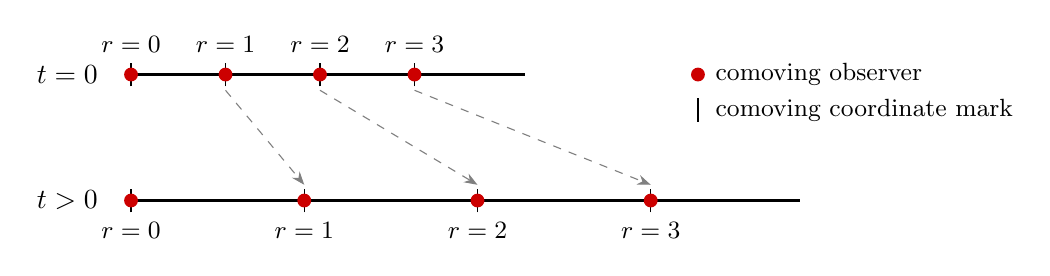
\begin{tikzpicture}[scale=1.0,>=Stealth]
  \node[left] at (-0.3,1.6) {$t=0$};
  \draw[thick] (0,1.6) -- (5,1.6);
  \foreach \x/\l in {0/0,1.2/1,2.4/2,3.6/3}{\draw (\x,1.45) -- (\x,1.75); \fill[red!80!black] (\x,1.6) circle (2.5pt); \node[above] at (\x,1.75) {\small $r=\l$};}
  \node[left] at (-0.3,0) {$t>0$};
  \draw[thick] (0,0) -- (8.5,0);
  \foreach \x/\l in {0/0,2.2/1,4.4/2,6.6/3}{\draw (\x,-0.15) -- (\x,0.15); \fill[red!80!black] (\x,0) circle (2.5pt); \node[below] at (\x,-0.15) {\small $r=\l$};}
  \foreach \a/\b in {1.2/2.2,2.4/4.4,3.6/6.6}{\draw[gray,dashed,->] (\a,1.4) -- (\b,0.2);}
  \fill[red!80!black] (7.2,1.6) circle (2.5pt); \node[right] at (7.3,1.6) {\small comoving observer};
  \draw (7.2,1.0) -- (7.2,1.3); \node[right] at (7.3,1.15) {\small comoving coordinate mark};
\end{tikzpicture}
\caption{Comoving observers (dots) sit at fixed comoving coordinates $r=0,1,2,3$, marked by the ticks of the coordinate grid. As the Universe expands ($t>0$), the grid itself is stretched: each observer keeps the same coordinate label, but the physical distance $a(t)\,\Delta r$ between neighbouring observers increases. (The marks are not physical rulers: a physical ruler, held together by non-gravitational forces, does not expand; it is the comoving grid that expands.)}
\label{fig:comoving}
\end{figure}

\section{Cosmological redshift}
Consider a fundamental observer $A$ at $\chi=0$ and a fundamental (comoving) source at $\chi_B$. The source emits a light pulse at time $t_e$, which is received by $A$ at $t_o$. Light travels along a radial null geodesic, $\dd s^2=0$ with $\dd\theta=\dd\phi=0$:
\[
  c^2\dd t^2-a^2(t)\dd\chi^2=0\quad\Longrightarrow\quad\int_{t_e}^{t_o}\frac{c\,\dd t}{a(t)}=\chi_B .
\]
At $t_e+\Delta t_e$ the source emits another pulse (e.g.\ the next wave crest, $\Delta t_e$ being the period of the photon), received at $t_o+\Delta t_o$. Since both observers are comoving, $\chi_B$ is the same constant, so
\[
  \Delta\int_{t_e}^{t_o}\frac{\dd t}{a(t)}=\frac{\Delta t_o}{a(t_o)}-\frac{\Delta t_e}{a(t_e)}=0
  \quad\Longrightarrow\quad\frac{\Delta t_o}{\Delta t_e}=\frac{a(t_o)}{a(t_e)} .
\]
\begin{keyresult}[Cosmological redshift]
\begin{equation}
  1+z\equiv\frac{\lambda_o}{\lambda_e}=\frac{f_e}{f_o}=\frac{a(t_o)}{a(t_e)}.
\end{equation}
In an expanding Universe ($a(t_o)>a(t_e)$) light from distant sources is redshifted: wavelengths are stretched together with the Universe.
\end{keyresult}

\begin{remarkbox}[Outlook: the Friedmann equations]
The FLRW metric follows from symmetry alone; the dynamics of $a(t)$ follows from the Einstein equations with a perfect-fluid source $T_{\mu\nu}=(\rho+p)u_\mu u_\nu-pg_{\mu\nu}$ at rest in comoving coordinates. One obtains (with $c=1$) the Friedmann equations
\[
  \Big(\frac{\dot a}{a}\Big)^2=\frac{8\pi\GN}{3}\rho-\frac{k}{a^2}+\frac\Lambda3,\qquad
  \frac{\ddot a}{a}=-\frac{4\pi\GN}{3}(\rho+3p)+\frac\Lambda3,
\]
which show explicitly that a positive cosmological constant (negative pressure) accelerates the expansion.
\end{remarkbox}

% =====================================================================
\chapter{Gravitational waves}\label{ch:gw}
% =====================================================================

\section{Interlude: electrodynamics}

Gravitational waves are best understood in analogy with electromagnetic waves, so we first recall how electrodynamics works (Gaussian units).
\begin{itemize}
\item Electromagnetism is described by the \textbf{Lorentz force} $m\ddot{\vec x}=e\vec E+\frac ec\dot{\vec x}\times\vec B$ and by \textbf{Maxwell's equations}
\[
  \nabla\cdot\vec E=4\pi\rho,\qquad\nabla\times\vec E=-\frac1c\frac{\pd\vec B}{\pd t},\qquad\nabla\cdot\vec B=0,\qquad\nabla\times\vec B=\frac{4\pi}{c}\vec J+\frac1c\frac{\pd\vec E}{\pd t},
\]
with $\rho$ the charge density and $\vec J$ the current density.
\item We typically introduce the \textbf{vector potential} $\vec A$, $\vec B=\nabla\times\vec A$ (which solves $\nabla\cdot\vec B=0$), and the \textbf{scalar potential} $\phi$, $\vec E+\frac1c\frac{\pd\vec A}{\pd t}=-\nabla\phi$ (which solves Faraday's law).
\item The $(4+4)$ equations can be written in a manifestly covariant form, and derived from an action $S=S_m+S_{\rm int}+S_{\rm EM}$ (free particle, interaction, electromagnetic field):
\begin{align*}
  &S_m=-mc\int_\Gamma\sqrt{\dd s^2},\\
  &S_{\rm int}=-\frac ec\int_\Gamma A_\mu\dd x^\mu=-\frac{1}{c^2}\int_\Omega J^\mu A_\mu\,\dd^4\Omega,\\
  &S_{\rm EM}=-\frac{1}{16\pi c}\int_\Omega F^{\mu\nu}F_{\mu\nu}\,\dd^4\Omega,
\end{align*}
where $\Gamma$ is the world-line, $\Omega$ a space-time region, and
\[
  F_{\mu\nu}\equiv\pd_\mu A_\nu-\pd_\nu A_\mu\ \text{(Faraday tensor)},\qquad A^\mu\equiv(\phi,\vec A),\qquad J^\mu\equiv(\rho c,\rho\vec v).
\]
(The overall sign of $S_{\rm int}$ depends on the sign conventions for $A_\mu$.)
\item In particular, the inhomogeneous Maxwell equations read
\begin{equation}
  \pd_\mu F^{\mu\nu}=\frac{4\pi}{c}J^\nu
\end{equation}
(the sign depends on conventions), and they are invariant under \textbf{gauge transformations} $A_\mu(x)\to A'_\mu(x)=A_\mu(x)+\pd_\mu\Lambda(x)$, with $\Lambda$ an arbitrary function, since $F_{\mu\nu}$ is.
\item For example, we can choose $A_\mu$ such that $\pd_\mu A^\mu=0$ (\textbf{Lorenz gauge}). This is always possible: if $\pd_\mu A^\mu\neq0$, choose $\Lambda$ with $\Box\Lambda=-\pd_\mu A^\mu$. In this gauge Maxwell's equations become wave equations, $\Box A^\nu=\frac{4\pi}{c}J^\nu$: in vacuum, electromagnetic waves.
\end{itemize}
\textbf{Why all this?} In GR the same things happen, because the Einstein equations work in every coordinate system: we have the freedom to choose coordinates, and the physics remains unchanged. This freedom plays the role of the gauge freedom of electrodynamics, and with a clever choice (a ``gauge'') the linearised Einstein equations become wave equations.

\section{Linearised gravity}

Same idea as in the Newtonian limit: we expand
\begin{equation}
  g_{\mu\nu}=\eta_{\mu\nu}+h_{\mu\nu},\qquad|h_{\mu\nu}|\ll1 ,
\end{equation}
where $h_{\mu\nu}$ is a perturbation, and we drop all terms of order $h^2$, $(\pd h)^2$, $h\,\pd^2h$, \dots Remember that the inverse metric has a minus sign:
\begin{equation}
  g^{\mu\nu}=\eta^{\mu\nu}-h^{\mu\nu}+\order{h^2}
\end{equation}
(proof: writing $g^{\mu\nu}=\eta^{\mu\nu}+H^{\mu\nu}$, $g_{\mu\nu}g^{\nu\rho}=\delta_\mu{}^\rho+\eta_{\mu\nu}H^{\nu\rho}+h_{\mu\nu}\eta^{\nu\rho}+\order{hH}=\delta_\mu{}^\rho$ requires $H_\mu{}^\rho=-h_\mu{}^\rho$, i.e.\ $H^{\mu\nu}=-h^{\mu\nu}$).

\begin{remarkbox}[Remarks]
\begin{enumerate}[label=(\roman*),nosep]
\item In linearised gravity we raise and lower indices of $h$ (and of all first-order quantities) with $\eta^{\mu\nu}$, $\eta_{\mu\nu}$; the difference with $g$ is of higher order.
\item Summary: $g_{\mu\nu}=\eta_{\mu\nu}+h_{\mu\nu}$, $g^{\mu\nu}=\eta^{\mu\nu}-h^{\mu\nu}$, $g^\mu{}_\nu=\delta^\mu{}_\nu\ (=\eta^\mu{}_\nu)$, where $h^\mu{}_\nu=\eta^{\mu\alpha}h_{\alpha\nu}$ and $h^{\mu\nu}=\eta^{\mu\alpha}\eta^{\nu\beta}h_{\alpha\beta}$; so that $g_{\mu\nu}g^{\nu\rho}=\delta_\mu{}^\rho$ to first order.
\item In linearised gravity, $h_{\mu\nu}$ is a tensor \emph{only under Lorentz transformations} (not under general ones). Under $x'^\mu=L^\mu{}_\nu x^\nu$, $g'_{\mu\nu}=L_\mu{}^\alpha L_\nu{}^\beta(\eta_{\alpha\beta}+h_{\alpha\beta})=\eta_{\mu\nu}+L_\mu{}^\alpha L_\nu{}^\beta h_{\alpha\beta}$, so $h$ transforms as a Lorentz tensor; a general transformation would destroy the split ``background $\eta$ $+$ small perturbation''.
\end{enumerate}
\end{remarkbox}

\paragraph{Gauge transformations.} The split does survive \emph{infinitesimal} coordinate transformations $x'^\mu=x^\mu+\xi^\mu(x)$, with $\xi$ of the same order as $h$. By Problem Sheet 2 (Killing equation), $g'_{\mu\nu}(x')=g_{\mu\nu}(x)-g_{\mu\alpha}\pd_\nu\xi^\alpha-g_{\alpha\nu}\pd_\mu\xi^\alpha$; evaluating both sides at the same coordinate value and dropping second-order terms ($\xi^\alpha\pd_\alpha h$, $h\pd\xi$):
\begin{equation}
  h'_{\mu\nu}=h_{\mu\nu}-\pd_\mu\xi_\nu-\pd_\nu\xi_\mu .
  \label{eq:gauge-h}
\end{equation}
This is the analogue of $A_\mu\to A_\mu+\pd_\mu\Lambda$: $h_{\mu\nu}$ and $h'_{\mu\nu}$ describe the same physical situation.

\section{The Einstein equations in linearised gravity}

\paragraph{Christoffel symbols.} By definition $\Ga{\lambda}{\sigma}{\rho}=\frac12g^{\lambda\mu}(\pd_\sigma g_{\rho\mu}+\pd_\rho g_{\sigma\mu}-\pd_\mu g_{\sigma\rho})$. The bracket contains no $\eta$'s (their derivatives vanish), so it is already linear in $h$ and we can replace $g^{\lambda\mu}\to\eta^{\lambda\mu}$:
\begin{equation}
  \Ga{\lambda}{\sigma}{\rho}\simeq\frac12\eta^{\lambda\mu}\big(\pd_\sigma h_{\rho\mu}+\pd_\rho h_{\sigma\mu}-\pd_\mu h_{\sigma\rho}\big).\tag{1}
\end{equation}
\paragraph{Riemann tensor.} $\Riem{\lambda}{\mu}{\sigma}{\nu}=\pd_\sigma\Ga{\lambda}{\nu}{\mu}-\pd_\nu\Ga{\lambda}{\sigma}{\mu}+\Gamma\Gamma-\Gamma\Gamma$, and the $\Gamma\Gamma$ terms are at least quadratic, $\order{h^2}$, so we remove them:
\begin{equation}
  \Riem{\lambda}{\mu}{\sigma}{\nu}\simeq\pd_\sigma\Ga{\lambda}{\nu}{\mu}-\pd_\nu\Ga{\lambda}{\sigma}{\mu}.\tag{2}
\end{equation}
Inserting (1) in (2):
\begin{align*}
  \Riem{\lambda}{\mu}{\sigma}{\nu}&=\frac12\eta^{\lambda\alpha}\pd_\sigma\big(\pd_\nu h_{\mu\alpha}+\pd_\mu h_{\nu\alpha}-\pd_\alpha h_{\nu\mu}\big)-\frac12\eta^{\lambda\alpha}\pd_\nu\big(\pd_\sigma h_{\mu\alpha}+\pd_\mu h_{\sigma\alpha}-\pd_\alpha h_{\sigma\mu}\big)\\
  &=\frac12\eta^{\lambda\alpha}\big(\pd_\sigma\pd_\mu h_{\nu\alpha}-\pd_\sigma\pd_\alpha h_{\mu\nu}-\pd_\nu\pd_\mu h_{\sigma\alpha}+\pd_\nu\pd_\alpha h_{\mu\sigma}\big),
\end{align*}
since the terms $\pd_\sigma\pd_\nu h_{\mu\alpha}$ cancel. Lowering $\lambda$ with $\eta_{\lambda\alpha}$:
\begin{equation}
  R_{\lambda\mu\sigma\nu}\simeq\frac12\big(\pd_\sigma\pd_\mu h_{\lambda\nu}-\pd_\sigma\pd_\lambda h_{\mu\nu}-\pd_\nu\pd_\mu h_{\lambda\sigma}+\pd_\nu\pd_\lambda h_{\mu\sigma}\big).
\end{equation}
\textit{Comments:} (i) these expressions satisfy the symmetries and the Bianchi identities, with ordinary derivatives instead of covariant ones; (ii) $R_{\lambda\mu\sigma\nu}$ is already $\order h$; (iii) it is \textbf{gauge invariant}: under \eqref{eq:gauge-h} each term changes by third derivatives of $\xi$, which cancel in pairs because partial derivatives commute --- as it should, since curvature is physical.

\paragraph{Ricci tensor.} By definition $R_{\mu\nu}=g^{\lambda\sigma}R_{\lambda\mu\sigma\nu}\simeq\eta^{\lambda\sigma}R_{\lambda\mu\sigma\nu}$ (the correction is $\order{h^2}$):
\begin{equation}
  R_{\mu\nu}\simeq\frac12\big(\pd_\mu\pd^\lambda h_{\nu\lambda}+\pd_\nu\pd^\sigma h_{\sigma\mu}-\Box h_{\mu\nu}-\pd_\mu\pd_\nu h\big),
  \qquad h\equiv\eta^{\mu\nu}h_{\mu\nu},\quad\Box\equiv\eta^{\mu\nu}\pd_\mu\pd_\nu=\frac{1}{c^2}\pd_t^2-\nabla^2 .
\end{equation}
\paragraph{Ricci scalar.} By definition $R=g^{\mu\nu}R_{\mu\nu}\simeq\eta^{\mu\nu}R_{\mu\nu}=\frac12\big(\pd^\nu\pd^\lambda h_{\nu\lambda}+\pd^\mu\pd^\sigma h_{\sigma\mu}-\Box h-\Box h\big)$:
\begin{equation}
  R\simeq\pd^\mu\pd^\nu h_{\mu\nu}-\Box h .
\end{equation}

\paragraph{The Einstein equations.} The general form is $R_{\mu\nu}-\frac12g_{\mu\nu}R=8\pi\GN T_{\mu\nu}$ (we do not consider the $\Lambda$ term, and we set $c=1$). Applying the previous results:
\begin{equation}
  \frac12\big(\pd_\mu\pd^\lambda h_{\nu\lambda}+\pd_\nu\pd^\sigma h_{\sigma\mu}-\Box h_{\mu\nu}-\pd_\mu\pd_\nu h\big)-\frac12\eta_{\mu\nu}\big(\pd^\rho\pd^\sigma h_{\rho\sigma}-\Box h\big)=8\pi\GN T_{\mu\nu}.
  \label{eq:lin-efe-h}
\end{equation}
To simplify this complex equation, we introduce the \textbf{trace-reversed perturbation}
\begin{equation}
  \bar h_{\mu\nu}\equiv h_{\mu\nu}-\frac12\eta_{\mu\nu}h ,\qquad\text{whose trace is}\qquad\bar h\equiv\eta^{\mu\nu}\bar h_{\mu\nu}=h-\frac12\cdot4h=-h
\end{equation}
(hence the name). The relation is easily inverted: $h_{\mu\nu}=\bar h_{\mu\nu}-\frac12\eta_{\mu\nu}\bar h$.

\paragraph{The substitution, step by step.} Using $h_{\mu\nu}=\bar h_{\mu\nu}-\frac12\eta_{\mu\nu}\bar h$ and $h=-\bar h$:
\begin{align*}
  \pd_\mu\pd^\lambda h_{\nu\lambda}&=\pd_\mu\pd^\lambda\bar h_{\nu\lambda}-\tfrac12\pd_\mu\pd_\nu\bar h, &
  \pd_\nu\pd^\sigma h_{\sigma\mu}&=\pd_\nu\pd^\sigma\bar h_{\sigma\mu}-\tfrac12\pd_\nu\pd_\mu\bar h,\\
  \Box h_{\mu\nu}&=\Box\bar h_{\mu\nu}-\tfrac12\eta_{\mu\nu}\Box\bar h, &
  \pd_\mu\pd_\nu h&=-\pd_\mu\pd_\nu\bar h,\\
  \pd^\rho\pd^\sigma h_{\rho\sigma}&=\pd^\rho\pd^\sigma\bar h_{\rho\sigma}-\tfrac12\Box\bar h, &
  \Box h&=-\Box\bar h .
\end{align*}
Hence
\begin{align*}
  R_{\mu\nu}&=\frac12\Big(\pd_\mu\pd^\lambda\bar h_{\nu\lambda}+\pd_\nu\pd^\sigma\bar h_{\sigma\mu}\underbrace{-\pd_\mu\pd_\nu\bar h+\pd_\mu\pd_\nu\bar h}_{=0}-\Box\bar h_{\mu\nu}+\frac12\eta_{\mu\nu}\Box\bar h\Big),\\
  R&=\pd^\rho\pd^\sigma\bar h_{\rho\sigma}-\frac12\Box\bar h+\Box\bar h=\pd^\rho\pd^\sigma\bar h_{\rho\sigma}+\frac12\Box\bar h ,
\end{align*}
and
\[
  R_{\mu\nu}-\frac12\eta_{\mu\nu}R=\frac12\Big(\pd_\mu\pd^\lambda\bar h_{\nu\lambda}+\pd_\nu\pd^\sigma\bar h_{\sigma\mu}-\Box\bar h_{\mu\nu}+\underbrace{\tfrac12\eta_{\mu\nu}\Box\bar h-\tfrac12\eta_{\mu\nu}\Box\bar h}_{=0}-\eta_{\mu\nu}\pd^\rho\pd^\sigma\bar h_{\rho\sigma}\Big).
\]
\begin{keyresult}[Linearised Einstein equations]
\begin{equation}
  \pd_\mu\pd^\lambda\bar h_{\nu\lambda}+\pd_\nu\pd^\sigma\bar h_{\sigma\mu}-\Box\bar h_{\mu\nu}-\eta_{\mu\nu}\pd^\rho\pd^\sigma\bar h_{\rho\sigma}=16\pi\GN T_{\mu\nu}.
  \label{eq:lin-efe}
\end{equation}
\end{keyresult}
So far, we have introduced the most important results to study gravitational waves in the approximation of weak fields.

\section{The harmonic gauge}

Interestingly, linearised gravity does by no means uniquely specify the perturbation $h_{\mu\nu}$: the freedom to perform an infinitesimal coordinate transformation $x\to x'=x+\xi(x)$ gives rise to the \emph{gauge transformations} \eqref{eq:gauge-h}. Remember that in electrodynamics we introduce the Lorenz gauge $\pd_\mu A^\mu=0$. Analogously, we choose to work in the \textbf{harmonic} (or Hilbert, or de Donder) \textbf{gauge}:
\begin{equation}
  \boxed{\pd^\mu\bar h_{\mu\nu}=0}.
\end{equation}
(We go to the coordinate system in which $\bar h_{\mu\nu}$ has this form.) In this gauge the first, second and fourth terms of \eqref{eq:lin-efe} vanish, and the EFE become
\begin{equation}
  \boxed{\Box\bar h_{\mu\nu}=-16\pi\GN T_{\mu\nu}}\qquad\Big(=-\frac{16\pi\GN}{c^4}T_{\mu\nu}\Big).
\end{equation}
Thus $\bar h_{\mu\nu}$ represents a quantity that propagates as a wave at the vacuum speed of light, on a flat Minkowski background, and which is sourced by the energy--momentum tensor $T_{\mu\nu}$ of matter: in other words, $\bar h_{\mu\nu}$ is a \textbf{gravitational wave}.

\paragraph{Can we always reach the harmonic gauge?} Under \eqref{eq:gauge-h}, $h'=h-2\pd\cdot\xi$ and
\[
  \bar h'_{\mu\nu}=\bar h_{\mu\nu}-\pd_\mu\xi_\nu-\pd_\nu\xi_\mu+\eta_{\mu\nu}\pd^\alpha\xi_\alpha
  \quad\Longrightarrow\quad\pd^\mu\bar h'_{\mu\nu}=\pd^\mu\bar h_{\mu\nu}-\Box\xi_\nu-\pd_\nu\pd^\mu\xi_\mu+\pd_\nu\pd^\alpha\xi_\alpha=\pd^\mu\bar h_{\mu\nu}-\Box\xi_\nu .
\]
So choosing $\xi$ as a solution of $\Box\xi_\nu=\pd^\mu\bar h_{\mu\nu}$ (always possible: it is a wave equation with a source) brings us to the harmonic gauge. N.B.: if we are already in the harmonic gauge, a further transformation with $\Box\xi_\nu=0$ keeps us in the harmonic gauge (\emph{residual gauge freedom}).

\paragraph{Formal solution.} As in electrodynamics, the solution of the wave equation with the correct (causal) boundary conditions is the \emph{retarded} solution (the Green function of $\Box=\pd_t^2-\nabla^2$ gives $\psi=\int\frac{f(t-|\vec x-\vec x'|,\vec x')}{|\vec x-\vec x'|}\dd^3x'$ for $\Box\psi=4\pi f$):
\begin{equation}
  \bar h_{\mu\nu}(t,\vec x)=-4\GN\int\dd^3x'\,\frac{T_{\mu\nu}(t-|\vec x-\vec x'|,\vec x')}{|\vec x-\vec x'|}.
  \label{eq:retarded}
\end{equation}
The source is evaluated at the \emph{retarded time} $t-|\vec x-\vec x'|$ (the perturbation travels at the speed of light). (In the signature $(-,+,+,+)$, where $\Box=-\pd_t^2+\nabla^2$, the same physics is written $\Box\bar h_{\mu\nu}=-16\pi\GN T_{\mu\nu}$, $\bar h_{\mu\nu}=+4\GN\int T_{\mu\nu}/|\vec x-\vec x'|$; the sign difference just reflects $\eta\to-\eta$.) \textit{Check:} for a static non-relativistic source, $\bar h_{00}=-4\GN\int\frac{\rho}{|\vec x-\vec x'|}=4\Phi$, $\bar h=\bar h_{00}$, so $h_{00}=\bar h_{00}-\frac12\bar h=2\Phi$: the Newtonian limit $g_{00}=1+2\Phi$ is recovered.

\section{The transverse--traceless (TT) gauge}

$\bar h_{\mu\nu}$ is symmetric, so it has a priori $10$ independent components. The harmonic gauge condition (4 equations) reduces them to $6$. This means that the harmonic gauge condition does not uniquely specify the metric perturbation: indeed, any gauge transformation whose generator satisfies $\Box\xi_\mu=0$ preserves the gauge condition. To uniquely specify the metric perturbation, $4$ additional conditions can be imposed (one for each $\xi_\mu$), leaving $\boxed{2}$ independent, physical components (polarisations).

\paragraph{In practice (in vacuum).} Outside the sources $\Box\bar h_{\mu\nu}=0$, and we can use the residual freedom $\Box\xi_\mu=0$:
\begin{enumerate}
\item choose $\xi^0$ such that $\bar h=0$, i.e.\ $\bar h_{\mu\nu}$ is traceless (then $\bar h_{\mu\nu}=h_{\mu\nu}$);
\item choose the $\xi^i$ such that $h_{0i}=0$.
\end{enumerate}
Then the $\nu=0$ component of the harmonic condition gives $\pd^\mu h_{\mu0}=\pd^0h_{00}=0$: $h_{00}$ is time independent. A time-independent $h_{00}$ is just a static Newtonian field (as in \cref{ch:efe}), which does not describe a wave; for the wave part we set $h_{00}=0$. We are left with
\begin{equation}
  \boxed{h_{0\mu}=0,\qquad h=\eta^{\mu\nu}h_{\mu\nu}=0\ (\text{traceless}),\qquad\pd^jh_{ij}=0\ (\text{transverse})}.
\end{equation}
This is the \textbf{transverse--traceless gauge}, and we write $h^{\rm TT}_{\mu\nu}$.

\begin{remarkbox}[N.B.]
In vacuum ($\Box\bar h_{\mu\nu}=0$) one can always choose $\Box\xi_\mu=0$ appropriately, and the TT gauge is always possible. With matter ($\Box\bar h_{\mu\nu}\neq0$) it is not always possible to go to the TT gauge.
\end{remarkbox}

\paragraph{A convention for the spatial components.} With our signature $\eta_{ij}=-\delta_{ij}$, so $g_{ij}=-\delta_{ij}+h_{ij}$ and the proper spatial distance is $\dd l^2=(\delta_{ij}-h_{ij})\dd x^i\dd x^j$. To agree with the usual GW literature (written in $(-,+,+,+)$), from now on we denote by $h^{\rm TT}_{ij}$ the spatial \emph{strain}, i.e.\ the perturbation of the spatial metric $\dd l^2=(\delta_{ij}+h^{\rm TT}_{ij})\dd x^i\dd x^j$; in terms of the components of $h_{\mu\nu}=g_{\mu\nu}-\eta_{\mu\nu}$ this is $h^{\rm TT}_{ij}=-h_{ij}=h^i{}_j$. Since all equations are linear, $\Box h^{\rm TT}_{ij}=0$, transversality and tracelessness are unaffected.

\section{Propagation in vacuum: plane waves}

In vacuum,
\begin{equation}
  \Box h^{\rm TT}_{\mu\nu}=0 :
\end{equation}
it is a \textbf{wave equation}. We look for plane-wave solutions
\begin{equation}
  h^{\rm TT}_{\mu\nu}=\varepsilon_{\mu\nu}\,e^{ik_\alpha x^\alpha}\quad(\text{real part understood}),\qquad k^\mu=(\omega,\vec k),
\end{equation}
where $\varepsilon_{\mu\nu}$ is the (constant, symmetric) \emph{polarisation tensor}. Then:
\begin{itemize}
\item $\Box h=-k_\alpha k^\alpha h=0\Rightarrow k_\alpha k^\alpha=\omega^2-|\vec k|^2=0$: $\omega=|\vec k|$ (dispersion relation). The wave vector is null: \textbf{gravitational waves travel at the speed of light}.
\item Harmonic (transverse) condition: $k^\mu\varepsilon_{\mu\nu}=0$; TT: $\varepsilon_{0\mu}=0$, $\varepsilon^\mu{}_\mu=0$.
\end{itemize}
For propagation in the $z$-direction, $k^\mu=\omega(1,0,0,1)$, transversality gives $k^\mu\varepsilon_{\mu\nu}=\omega(\varepsilon_{0\nu}+\varepsilon_{3\nu})=0\Rightarrow\varepsilon_{3\nu}=0$; with $\varepsilon_{0\nu}=0$ and tracelessness, $\varepsilon_{22}=-\varepsilon_{11}$. Only two independent components remain, $h_+$ and $h_\times$:
\begin{equation}
  h^{\rm TT}_{\alpha\beta}=\begin{pmatrix}0&0&0&0\\0&h_+&h_\times&0\\0&h_\times&-h_+&0\\0&0&0&0\end{pmatrix}\cos\Big[\omega\Big(t-\frac zc\Big)\Big],
\end{equation}
where $h_+$, $h_\times$ are the amplitudes of the two polarisation modes (``plus'' and ``cross''). We can also write
\[
  h^{\rm TT}_{ij}=h_+\,\varepsilon^+_{ij}\cos[\omega(t-z/c)]+h_\times\,\varepsilon^\times_{ij}\cos[\omega(t-z/c)],\qquad
  \varepsilon^+=\begin{pmatrix}1&0&0\\0&-1&0\\0&0&0\end{pmatrix},\quad\varepsilon^\times=\begin{pmatrix}0&1&0\\1&0&0\\0&0&0\end{pmatrix}.
\]
Then the \textbf{line element} is
\begin{equation}
  \dd s^2=c^2\dd t^2-(1+h_+\cos\varphi)\dd x^2-(1-h_+\cos\varphi)\dd y^2-2h_\times\cos\varphi\,\dd x\,\dd y-\dd z^2,\qquad\varphi\equiv\omega\Big(t-\frac zc\Big).
\end{equation}

\section{Effects of gravitational waves on test particles}

\paragraph{1) A single free particle in the path of a GW.} A free particle obeys the geodesic equation $\ddot x^\mu+\Ga{\mu}{\nu}{\rho}\dot x^\nu\dot x^\rho=0$. Take a particle initially at rest at $\tau=0$: $\frac{\dd x^i}{\dd\tau}=0$. Then
\[
  \ddot x^\mu=-\Ga{\mu}{0}{0}\Big(\frac{\dd x^0}{\dd\tau}\Big)^2,\qquad\Ga{\mu}{0}{0}=\frac12\eta^{\mu\sigma}\big(\pd_0h_{0\sigma}+\pd_0h_{0\sigma}-\pd_\sigma h_{00}\big).
\]
In the TT gauge $h_{0\mu}=0$, so $\Ga{\mu}{0}{0}=0$ and $\ddot x^\mu=0$ (at $\tau=0$, and hence at all times): the particle stays at rest, i.e.\ at constant TT coordinates. \textbf{But} ``at rest'' with respect to its coordinate system: the TT coordinates are attached to the freely-falling particles themselves. To see a physical effect, we must consider the \emph{proper distance} between two particles.

\paragraph{2) Two particles at $(x_0,0,0)$ and $(-x_0,0,0)$.} How does the proper distance evolve? For a wave travelling along $z$ (at $z=0$), with the particles at fixed coordinates,
\begin{align}
  \Delta l&=\int_{-x_0}^{x_0}\sqrt{|\dd s^2|}=\int_{-x_0}^{x_0}\sqrt{|g_{xx}|}\,\dd x=\int_{-x_0}^{x_0}\sqrt{1+h_+\cos(\omega t)}\,\dd x\nonumber\\
  &\simeq L_0\Big[1+\frac12h_+\cos(\omega t)\Big],\qquad L_0=2x_0,
\end{align}
where we Taylor-expanded $\sqrt{1+\epsilon}\simeq1+\epsilon/2$. N.B.: for two particles at $(0,\pm x_0,0)$ instead, $\Delta l=L_0\big[1-\frac12h_+\cos(\omega t)\big]$.

\textit{Comments:}
\begin{enumerate}
\item The proper distance \emph{does} change, periodically, with the frequency of the wave: stretched along $x$ while squeezed along $y$, and vice versa half a period later.
\item $\Delta L\equiv\Delta l-L_0\propto L_0$ (the initial separation): the effect is a \emph{strain} $\Delta L/L_0=\frac12h_+\cos\omega t$. Since $h\sim10^{-21}$ for typical astrophysical sources, gravitational-wave detectors must be large (LIGO/Virgo arms are $3$--$4$\,km long, and measure $\Delta L\sim10^{-18}$\,m).
\item If you rotate the system by $45^\circ$, you get the same answer but with $h_\times$: the two polarisations differ by a $45^\circ$ rotation.
\item The effect on a ring of particles in the $xy$ plane is shown in \cref{fig:ring}. There is no effect along the direction of propagation: the waves are \emph{transverse}.
\end{enumerate}

\begin{figure}[ht]
\centering
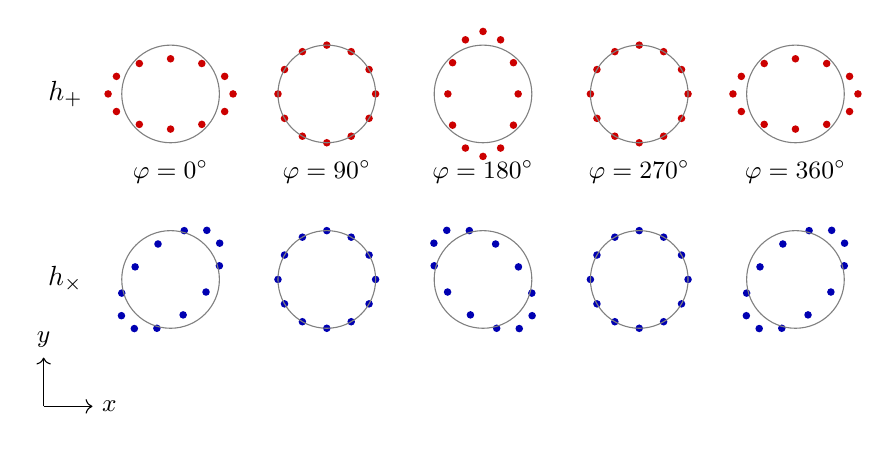
\begin{tikzpicture}[scale=0.62]
  \foreach \i/\ph in {0/0,1/90,2/180,3/270,4/360}{
    \begin{scope}[shift={(3.2*\i,0)}]
      \pgfmathsetmacro{\e}{0.28*cos(\ph)}
      \foreach \t in {0,30,...,330}{\fill[red!80!black] ({(1+\e)*cos(\t)},{(1-\e)*sin(\t)}) circle (2.2pt);}
      \draw[gray,thin] (0,0) circle (1);
      \node at (0,-1.6) {\small $\varphi=\ph^\circ$};
    \end{scope}
    \begin{scope}[shift={(3.2*\i,-3.8)}]
      \pgfmathsetmacro{\e}{0.28*cos(\ph)}
      \foreach \t in {0,30,...,330}{
        \pgfmathsetmacro{\X}{cos(\t)}\pgfmathsetmacro{\Y}{sin(\t)}
        \fill[blue!70!black] ({\X+\e*\Y},{\Y+\e*\X}) circle (2.2pt);}
      \draw[gray,thin] (0,0) circle (1);
    \end{scope}}
  \node[left] at (-1.6,0) {$h_+$};
  \node[left] at (-1.6,-3.8) {$h_\times$};
  \draw[->] (-2.6,-6.4) -- (-1.6,-6.4) node[right] {\small $x$};
  \draw[->] (-2.6,-6.4) -- (-2.6,-5.4) node[above] {\small $y$};
\end{tikzpicture}
\caption{Effect of a gravitational wave propagating along $z$ on a ring of free test particles in the $xy$ plane, over one period ($\varphi=\omega t$). Top: plus polarisation $h_+$ (the ring is alternately stretched along $x$ and squeezed along $y$, and vice versa). Bottom: cross polarisation $h_\times$ (the same pattern rotated by $45^\circ$). The deformation is enormously exaggerated.}
\label{fig:ring}
\end{figure}

\section{Generation of gravitational waves: Einstein's quadrupole formula}

We now describe the generation of gravitational waves by isolated systems. For each component of $\bar h_{\mu\nu}$ the linear equation can be solved by \eqref{eq:retarded} (in the harmonic gauge).

\paragraph{Compact source, far away.} Assume a compact source observed from far away: $|\vec x-\vec x'|\simeq|\vec x|\equiv r$ for all points $\vec x'$ of the source (and, for slowly moving sources, the retardation across the source can be neglected). Then
\begin{equation}
  \bar h_{\mu\nu}(t,r)\simeq-\frac{4\GN}{r}\int\dd^3x'\,T_{\mu\nu}(t-r,\vec x').
\end{equation}
In linearised theory $h_{\mu\nu}$ and $T_{\mu\nu}$ are of the same order (Einstein equations), so the conservation law $D_\mu T^{\mu\nu}=0$ reduces to $\pd_\mu T^{\mu\nu}=0$ at this order. Starting from this, one can play around with the components ($c=1$; all integrals over a volume $V$ containing the source, on whose boundary $T^{\mu\nu}=0$).

\paragraph{1. $\nu=0$ and $\nu=i$: conserved quantities.} $\pd_\mu T^{\mu0}=0\Rightarrow\pd_0T^{00}=-\pd_kT^{k0}$. Integrating over the region where $T^{\mu\nu}\neq0$, by Gauss' theorem
\[
  \frac{\pd}{\pd t}\int_VT^{00}\dd^3x=-\int_V\pd_kT^{k0}\dd^3x=-\oint_{\pd V}T^{k0}\dd\Sigma_k=0 .
\]
So $\int T^{00}\dd^3x$ is constant (total energy/mass), and similarly $\int T^{0i}\dd^3x$ (total momentum). Hence $\bar h^{0\nu}$ is constant in time: it is the static (Newtonian) part of the field and it does not contribute to the waves; we decide to put $\bar h^{0\nu}=0$ for the radiative part.

\paragraph{2. Integrals of $T^{ij}$.} $\pd_\mu T^{\mu i}=0\Rightarrow\pd_0T^{0i}=-\pd_kT^{ki}$. Multiply by $x^j$ and integrate, integrating by parts:
\begin{align*}
  \frac{\pd}{\pd t}\int_Vx^jT^{0i}\dd^3x&=-\int_Vx^j\pd_kT^{ki}\dd^3x=-\int_V\pd_k\big(x^jT^{ki}\big)\dd^3x+\int_VT^{ki}\frac{\pd x^j}{\pd x^k}\dd^3x\\
  &=-\oint_{\pd V}x^jT^{ki}\dd\Sigma_k+\int_VT^{ji}\dd^3x=\int_VT^{ij}\dd^3x ,
\end{align*}
since $T$ vanishes on the boundary and $\pd x^j/\pd x^k=\delta^j{}_k$. But $T^{\mu\nu}$ is symmetric, so we get the same result with $i\leftrightarrow j$. Adding the two:
\begin{equation}
  \frac{\pd}{\pd t}\int_V\big(T^{i0}x^j+T^{j0}x^i\big)\dd^3x=2\int_VT^{ij}\dd^3x .\tag{$\star$}
\end{equation}
\paragraph{3. Second moment of $T^{00}$.} $\pd_\mu T^{\mu0}=0\Rightarrow\pd_0T^{00}=-\pd_kT^{k0}$. Multiply by $x^ix^j$ and integrate by parts:
\[
  \int_Vx^ix^j\pd_0T^{00}\dd^3x=-\int_Vx^ix^j\pd_kT^{k0}\dd^3x=\int_VT^{k0}\frac{\pd(x^ix^j)}{\pd x^k}\dd^3x=\int_V\big(T^{i0}x^j+T^{j0}x^i\big)\dd^3x .
\]
Hence $\frac{\pd}{\pd t}\int x^ix^jT^{00}=\int(T^{i0}x^j+T^{j0}x^i)$, and differentiating once more and using ($\star$):
\begin{equation}
  \frac{\pd^2}{\pd t^2}\int_Vx^ix^jT^{00}\dd^3x=2\int_VT^{ij}\dd^3x .
\end{equation}

\begin{definition}{Quadrupole moment of the source}{quadrupole}
\begin{equation}
  Q^{ij}(t)\equiv\int_VT^{00}(t,\vec x)\,x^ix^j\,\dd^3x ,\qquad\ddot Q^{ij}\equiv\frac{\pd^2Q^{ij}}{\pd t^2}.
\end{equation}
\end{definition}
Therefore $\int T^{ij}\dd^3x=\frac12\ddot Q^{ij}$ and the solution of the linearised EFE is
\begin{equation}
  \bar h_{\mu0}=0,\qquad\bar h_{ij}=-\frac{2\GN}{r}\ddot Q_{ij}(t-r)\quad\Longleftrightarrow\quad\text{strain}\ \ \frac{2\GN}{r}\ddot Q_{ij}(t-r)
\end{equation}
(using the strain convention of the previous section, $\bar h^{\rm strain}_{ij}=-\bar h_{ij}$). Note: if the source has spherical symmetry, $Q_{ij}\propto\delta_{ij}$ with $\ddot Q_{ij}$ pure trace, which is removed by the TT projection below: spherically symmetric collapses or pulsations do not emit gravitational waves (in agreement with Birkhoff's theorem).

\paragraph{Comparison with electromagnetism.} In electrodynamics the leading radiation is \emph{dipole} radiation, $\propto\ddot{\vec d}$ with $\vec d=\int\rho_e\vec x$. The gravitational analogue, the mass dipole $\int T^{00}\vec x$, is (proportional to) the position of the centre of mass, whose second derivative vanishes by momentum conservation (item 1 above). Likewise the ``magnetic dipole'' analogue is the conserved angular momentum. Hence the leading gravitational radiation is \textbf{quadrupolar}, which is much weaker.

\paragraph{Moving to the TT gauge.} We now want to preserve the harmonic gauge while switching to the TT gauge. For a wave travelling radially, along $\vec n=\vec x/r$:
\begin{itemize}[nosep]
\item already $\bar h_{\mu0}=0$;
\item traceless condition: $\delta^{ij}h^{\rm TT}_{ij}=0$;
\item transverse condition: $n^ih^{\rm TT}_{ij}=0$.
\end{itemize}
In order to do that we introduce the projector
\begin{equation}
  P_{ij}\equiv\delta_{ij}-n_in_j ,
\end{equation}
which is symmetric and projects vectors onto the plane transverse to $\vec n$: $P_{ij}n^j=n_i-n_in_jn^j=n_i-n_i=0$, and $P_{ik}P_{kj}=P_{ij}$ (it is a projector); its trace is $P_{ii}=3-1=2$. We then introduce
\begin{equation}
  \Lambda_{ij,k\ell}\equiv P_{ik}P_{j\ell}-\frac12P_{ij}P_{k\ell},\qquad h^{\rm TT}_{ij}=\Lambda_{ij,k\ell}\,\bar h_{k\ell}.
\end{equation}
\begin{exercise}{$h^{\rm TT}_{ij}$ is transverse and traceless}{tt-proof}
\textit{Transverse:} $n^ih^{\rm TT}_{ij}=\big(n^iP_{ik}P_{j\ell}-\frac12n^iP_{ij}P_{k\ell}\big)\bar h_{k\ell}=0$, since $n^iP_{ik}=0$ and $n^iP_{ij}=0$.

\textit{Traceless:} $\delta^{ij}h^{\rm TT}_{ij}=\big(P_{ik}P_{i\ell}-\frac12P_{ii}P_{k\ell}\big)\bar h_{k\ell}=\big(P_{k\ell}-\frac12\cdot2\,P_{k\ell}\big)\bar h_{k\ell}=0$, using $P_{ik}P_{i\ell}=P_{k\ell}$ (projector) and $P_{ii}=2$.

Moreover $\Lambda$ is itself a projector ($\Lambda_{ij,k\ell}\Lambda_{k\ell,mn}=\Lambda_{ij,mn}$), so applying it to a tensor that is already TT leaves it unchanged.
\end{exercise}

\begin{keyresult}[Einstein's quadrupole formula]
In the end:
\begin{equation}
  h^{\rm TT}_{\mu0}=0,\qquad h^{\rm TT}_{ij}(t,\vec x)=\frac{2\GN}{c^4r}\,\ddot Q^{\rm TT}_{ij}\Big(t-\frac rc\Big),\qquad Q^{\rm TT}_{ij}=\Lambda_{ij,k\ell}\,Q_{k\ell}.
\end{equation}
\end{keyresult}

\section{Example: a binary system in a circular orbit}

Consider two masses $m_1$, $m_2$ in a circular orbit around their centre of mass (CM), in the $xy$ plane (\cref{fig:binary}). Let $M=m_1+m_2$, $R=r_1+r_2$ the separation, and $\mu=m_1m_2/M$ the reduced mass. With the CM at the origin, $m_1\vec r_1+m_2\vec r_2=0$, so $r_1=\frac{m_2}{M}R$, $r_2=\frac{m_1}{M}R$.

\begin{figure}[ht]
\centering
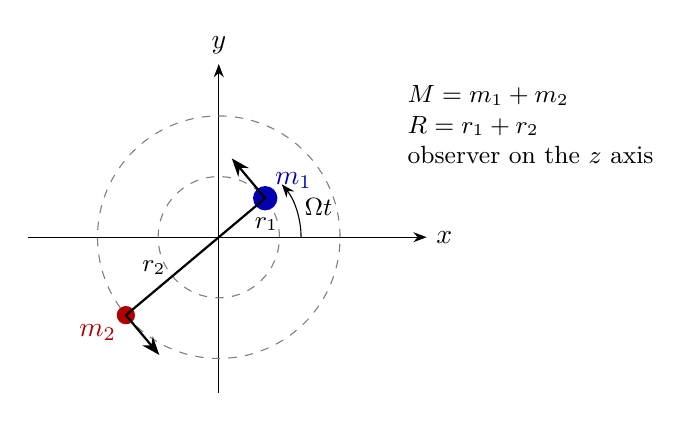
\begin{tikzpicture}[scale=1.1,>=Stealth]
  \draw[->] (-2.2,0) -- (2.4,0) node[right] {$x$};
  \draw[->] (0,-1.8) -- (0,2.0) node[above] {$y$};
  \draw[dashed,gray] (0,0) circle (0.7);
  \draw[dashed,gray] (0,0) circle (1.4);
  \fill[blue!70!black] (40:0.7) circle (4pt) node[above right] {$m_1$};
  \fill[red!70!black] (220:1.4) circle (3pt) node[below left] {$m_2$};
  \draw[thick] (220:1.4) -- (40:0.7);
  \node[font=\small] at (0.55,0.15) {$r_1$};
  \node[font=\small] at (-0.75,-0.35) {$r_2$};
  \draw[->,thick] (40:0.7) -- ++(130:0.6);
  \draw[->,thick] (220:1.4) -- ++(310:0.6);
  \draw[->] (0.95,0) arc (0:40:0.95); \node[font=\small] at (1.15,0.35) {$\Omega t$};
  \node[align=left,font=\small] at (3.6,1.3) {$M=m_1+m_2$\\$R=r_1+r_2$\\ observer on the $z$ axis};
\end{tikzpicture}
\caption{A binary system in a circular orbit in the $xy$ plane, around its centre of mass at the origin. The observer is located far away on the $z$ axis.}
\label{fig:binary}
\end{figure}

\paragraph{1) Newtonian orbit.} The gravitational force provides the centripetal force:
\[
  \frac{\GN m_1m_2}{R^2}=m_1\Omega^2r_1=m_1\Omega^2\frac{m_2}{M}R\quad\Longrightarrow\quad\Omega^2=\frac{\GN M}{R^3}\quad\text{(Kepler's third law)}.
\]
\paragraph{2) Trajectories.}
\[
  \vec x_1=\begin{pmatrix}r_1\cos\Omega t\\ r_1\sin\Omega t\\0\end{pmatrix},\qquad
  \vec x_2=\begin{pmatrix}-r_2\cos\Omega t\\ -r_2\sin\Omega t\\0\end{pmatrix}.
\]
\paragraph{3) Quadrupole moment.} For point masses (non-relativistic) $T^{00}=\sum_{a=1}^2m_ac^2\,\delta(x-x_a)\delta(y-y_a)\delta(z)$ (we set $c=1$ below), so that
\[
  Q^{ij}(t)=\int_VT^{00}(t,\vec x)x^ix^j\dd^3x=\sum_am_a\,x_a^i(t)\,x_a^j(t).
\]
For instance, using $m_1r_1^2+m_2r_2^2=\frac{m_1m_2^2+m_2m_1^2}{M^2}R^2=\mu R^2$:
\[
  Q_{xx}=m_1x_1^2+m_2x_2^2=\mu R^2\cos^2\Omega t=\frac{\mu R^2}{2}\cos2\Omega t+\text{const},
\]
and similarly $Q_{yy}=\mu R^2\sin^2\Omega t=-\frac{\mu R^2}2\cos2\Omega t+\text{const}$, $Q_{xy}=\mu R^2\sin\Omega t\cos\Omega t=\frac{\mu R^2}{2}\sin2\Omega t$, $Q_{iz}=0$. In the end
\begin{equation}
  Q_{ij}=\frac{\mu R^2}{2}\begin{pmatrix}\cos2\Omega t&\sin2\Omega t&0\\ \sin2\Omega t&-\cos2\Omega t&0\\0&0&0\end{pmatrix}+\text{const},
  \qquad\ddot Q_{ij}=-2\mu R^2\Omega^2\begin{pmatrix}\cos2\Omega t&\sin2\Omega t&0\\ \sin2\Omega t&-\cos2\Omega t&0\\0&0&0\end{pmatrix}.
\end{equation}
\paragraph{4) TT projection.} Assume the observer is along the $z$ axis: unit vector $\vec n=(0,0,1)$ and projector $P_{ij}=\delta_{ij}-n_in_j=\mathrm{diag}(1,1,0)$. Then, e.g.,
\[
  Q^{\rm TT}_{xx}=\Lambda_{xx,k\ell}Q_{k\ell}=\Big(P_{xk}P_{x\ell}-\frac12P_{xx}P_{k\ell}\Big)Q_{k\ell}=\Big(P_{xx}^2-\frac12P_{xx}^2\Big)Q_{xx}-\frac12P_{xx}P_{yy}Q_{yy}=\frac12(Q_{xx}-Q_{yy}),
\]
and similarly $Q^{\rm TT}_{yy}=-\frac12(Q_{xx}-Q_{yy})$, $Q^{\rm TT}_{xy}=Q_{xy}$, $Q^{\rm TT}_{iz}=0$:
\[
  Q^{\rm TT}_{ij}=\begin{pmatrix}\frac12(Q_{xx}-Q_{yy})&Q_{xy}&0\\ Q_{xy}&-\frac12(Q_{xx}-Q_{yy})&0\\0&0&0\end{pmatrix}.
\]
(For this particular source $Q_{ij}$ restricted to the $xy$ plane is already traceless up to a constant, so the projection only removes the constant part.)

\paragraph{5) The waveform.} So $h^{\rm TT}_{\mu0}=0$ and $h^{\rm TT}_{ij}=\frac{2\GN}{r}\ddot Q^{\rm TT}_{ij}(t-r)$, which has exactly the plane-wave form of the previous sections with $r=z$:
\begin{equation}
  h^{\rm TT}_{\mu\nu}=\begin{pmatrix}0&0&0&0\\0&h_+&h_\times&0\\0&h_\times&-h_+&0\\0&0&0&0\end{pmatrix},
\end{equation}
\begin{keyresult}[Gravitational waves from a circular binary (observer on the axis)]
\begin{equation}
  h_+(t)=-\frac{4\GN\mu R^2\Omega^2}{c^4z}\cos\Big[2\Omega\Big(t-\frac zc\Big)\Big],\qquad
  h_\times(t)=-\frac{4\GN\mu R^2\Omega^2}{c^4z}\sin\Big[2\Omega\Big(t-\frac zc\Big)\Big].
\end{equation}
\end{keyresult}
\textit{Comments:} the waves have \textbf{twice the orbital frequency} ($\omega_{\rm GW}=2\Omega$), since the mass distribution returns to the same configuration after half an orbit; the two polarisations are out of phase by $\pi/2$ (circular polarisation, for an observer on the axis); the amplitude decreases as $1/r$. Using Kepler's law, $\mu R^2\Omega^2=\mu(\GN M\Omega)^{2/3}$, and for a typical stellar-mass binary at $\sim100$\,Mpc one gets $h\sim10^{-21}$--$10^{-22}$. The energy carried away by these waves makes the orbit shrink (as observed in the Hulse--Taylor binary pulsar), until the two objects merge: the signals detected by LIGO/Virgo since 2015.


\appendix
% =====================================================================
\chapter{Summary of key formulae}\label{app:summary}
% =====================================================================
Signature $(+,-,-,-)$; $c=1$ unless stated otherwise.

\section*{Tensors and metric}
\begin{itemize}[nosep]
\item Vector: $V'^\mu=\frac{\pd x'^\mu}{\pd x^\nu}V^\nu$; covector: $U'_\mu=\frac{\pd x^\nu}{\pd x'^\mu}U_\nu$; metric: $g'_{\mu\nu}=\frac{\pd x^\alpha}{\pd x'^\mu}\frac{\pd x^\beta}{\pd x'^\nu}g_{\alpha\beta}$.
\item Line element $\dd s^2=g_{\mu\nu}\dd x^\mu\dd x^\nu=c^2\dd\tau^2$; $V_\mu=g_{\mu\nu}V^\nu$; $g_{\mu\nu}g^{\nu\rho}=\delta_\mu{}^\rho$; invariant volume $\sqrt{|g|}\,\dd^4x$.
\end{itemize}
\section*{Connection and geodesics}
\begin{itemize}[nosep]
\item $\Ga{\lambda}{\sigma}{\rho}=\frac12g^{\lambda\mu}(\pd_\sigma g_{\rho\mu}+\pd_\rho g_{\sigma\mu}-\pd_\mu g_{\sigma\rho})$.
\item $D_\mu V^\nu=\pd_\mu V^\nu+\Ga{\nu}{\mu}{\lambda}V^\lambda$, $D_\mu U_\nu=\pd_\mu U_\nu-\Ga{\lambda}{\mu}{\nu}U_\lambda$, $D_\alpha g_{\mu\nu}=0$.
\item Geodesics: $\ddot x^\mu+\Ga{\mu}{\nu}{\rho}\dot x^\nu\dot x^\rho=0$, from $\mathcal L=\frac12g_{\mu\nu}\dot x^\mu\dot x^\nu$.
\end{itemize}
\section*{Curvature}
\begin{itemize}[nosep]
\item $\Riem{\rho}{\sigma}{\mu}{\nu}=\pd_\mu\Ga{\rho}{\nu}{\sigma}-\pd_\nu\Ga{\rho}{\mu}{\sigma}+\Ga{\rho}{\mu}{\lambda}\Ga{\lambda}{\nu}{\sigma}-\Ga{\rho}{\nu}{\lambda}\Ga{\lambda}{\mu}{\sigma}$, $[D_\mu,D_\nu]V^\rho=\Riem{\rho}{\sigma}{\mu}{\nu}V^\sigma$.
\item $R_{\mu\nu\rho\sigma}=-R_{\nu\mu\rho\sigma}=-R_{\mu\nu\sigma\rho}=R_{\rho\sigma\mu\nu}$, $R_{\mu[\nu\rho\sigma]}=0$, Bianchi $D_{[\lambda}R^\mu{}_{|\nu|\rho\sigma]}=0$; 20 components in 4D.
\item $R_{\mu\nu}=\Riem{\rho}{\mu}{\rho}{\nu}$, $R=g^{\mu\nu}R_{\mu\nu}$, $G_{\mu\nu}=R_{\mu\nu}-\frac12g_{\mu\nu}R$, $D^\mu G_{\mu\nu}=0$.
\item Geodesic deviation: $\frac{D^2X^\mu}{\dd\lambda^2}=\Riem{\mu}{\nu}{\rho}{\sigma}T^\nu T^\rho X^\sigma$.
\end{itemize}
\section*{Matter and field equations}
\begin{itemize}[nosep]
\item Perfect fluid: $T^{\mu\nu}=(\rho+p)u^\mu u^\nu-pg^{\mu\nu}$; $D_\mu T^{\mu\nu}=0$.
\item Newtonian limit: $g_{00}=1+2\Phi/c^2$.
\item EFE: $R_{\mu\nu}-\frac12g_{\mu\nu}R-\Lambda g_{\mu\nu}=\frac{8\pi\GN}{c^4}T_{\mu\nu}$; equivalently $R_{\mu\nu}=8\pi\GN(T_{\mu\nu}-\frac12Tg_{\mu\nu})$ (for $\Lambda=0$).
\end{itemize}
\section*{Solutions}
\begin{itemize}[nosep]
\item Schwarzschild: $\dd s^2=(1-\rs/r)c^2\dd t^2-(1-\rs/r)^{-1}\dd r^2-r^2\dd\Omega^2$, $\rs=2\GN M/c^2$.
\item Light deflection $\delta\phi=4\GN M/(c^2b)$; perihelion advance $6\pi\GN M/(c^2a(1-e^2))$ per orbit; Shapiro delay $\frac{4\GN M}{c^3}[1+\ln(4r_Ar_B/R^2)]$.
\item Kruskal: $\dd s^2=-\frac{4\rs^3}{r}e^{-r/\rs}\dd U\dd V-r^2\dd\Omega^2$, $UV=(r/\rs-1)e^{r/\rs}$, $V/U=e^{ct/\rs}$.
\item FLRW: $\dd s^2=c^2\dd t^2-a^2(t)\big[\frac{\dd r^2}{1-kr^2}+r^2\dd\Omega^2\big]$, $1+z=a(t_o)/a(t_e)$.
\item Linearised gravity: $\bar h_{\mu\nu}=h_{\mu\nu}-\frac12\eta_{\mu\nu}h$, harmonic gauge $\pd^\mu\bar h_{\mu\nu}=0$, $\Box\bar h_{\mu\nu}=-16\pi\GN T_{\mu\nu}$; quadrupole formula $h^{\rm TT}_{ij}=\frac{2\GN}{c^4r}\ddot Q^{\rm TT}_{ij}(t-r/c)$.
\end{itemize}


\end{document}
